
% Document class `report-template` accepts either project-plan or final-report option in
% []. This will change the title page as necessary.
% \documentclass[project-plan]{report-template}
\documentclass[final-report]{report-template}

\usepackage{caption}
\usepackage{subcaption}
\usepackage{float}
\usepackage{graphicx}
\usepackage{amsmath}
\usepackage{blindtext}
\usepackage{newtxtext,newtxmath}
\usepackage{cite}      
\usepackage{float}
\usepackage{tikz}
\usetikzlibrary{arrows.meta,positioning,fit,shapes.geometric}
\usepackage{booktabs}
% \usepackage{multirow}
\bibliographystyle{ieeetr}  % or another style you prefer (see below)
% \usepackage[hidelinks]{hyperref} % 可选
% \usepackage[
%   backend=biber,
%   style=ieee,
%   doi=true,
%   url=true,
%   eprint=true
% ]{biblatex}
% \addbibresource{reference.bib} 
% \bibliography{dreambirds_references} % <-- no .bib extension


% Colors for Gantt chart
\usepackage{xcolor}% Morandi-inspired colors
\definecolor{morblue}{HTML}{9BA8B3}
\definecolor{morgreen}{HTML}{AFC1A8}
\definecolor{morrose}{HTML}{D8B4A6}
\definecolor{moryellow}{HTML}{E3CDA4}
\definecolor{morred}{HTML}{C8A8A8}
\definecolor{morpurple}{HTML}{B8A8C8}
\definecolor{mororange}{HTML}{D4B896}
\definecolor{morbrown}{HTML}{A89B8C}
\definecolor{morgray}{HTML}{9B9B9B}
\definecolor{morwhite}{HTML}{F5F2F0}
\definecolor{morblack}{HTML}{3A3A3A}
\usepackage{pgfgantt}



\graphicspath{{./figures/}}

% Metadata used for the title page - please modify.
\university{Imperial College London}
\department{Department of Earth Science and Engineering}
\course{MSc in Applied Computational Science and Engineering}
% \title{Dreambirds in Motion: AI-Driven Temporal Consistency in Surreal Video}
\title{Dreambirds in Motion:\\ 
AI-driven Surreal Video Generation with Pose-Guided Temporal Consistency}
\author{Xinyu (Marceline) Cheng}
\email{xinyu.cheng24@imperial.ac.uk}
\githubusername{esemsc-xc924}
\supervisors{Prof. Christopher Pain\\
             Prof. James Coupe (Royal College of Art)}
\repository{https://github.com/ese-msc-2024/irp-xc924}

\begin{document}

\maketitlepage 

\tableofcontents  
\newpage         



% \begin{abstract}
% Traditional bird motion video production faces significant challenges, including high costs, technical barriers, and the scarcity of skeletal motion datasets for AI model training. This study presents an end-to-end framework for generating controllable surreal bird motion videos from static images through a multi-stage pipeline integrating Motion Diffusion Model (MDM) and generative video synthesis models. The system first employs HRNet for accurate skeletal keypoint detection, then leverages MDM to generate motion sequences in the CUB-15 representation, conditioned on initial inputs for precise control. To synthesise videos, the pipeline primarily utilises AnimateDiff with ControlNet conditioning, which renders the skeletons into surreal animations while preserving distinctive visual traits. To support the workflow, we develop a motion analysis framework and an automatic prompt generation module to address adaptation challenges for surreal bird data. Experiments demonstrate improvements in motion accuracy, temporal consistency, and feature preservation, highlighting a promising pathway for AI-driven wildlife video generation with enhanced artistic controllability.
% \end{abstract}

\begin{abstract}
Producing bird motion videos with AI remains challenging due to high costs, technical barriers, and the scarcity of temporally annotated skeletal datasets. This study presents an end-to-end framework for generating surreal bird motion videos from static images through a three-stage pipeline. First, HRNet detects avian keypoints in the CUB-15 skeletal representation. Second, a Motion Diffusion Model (MDM) generates temporally coherent pose sequences conditioned on initial frames and action labels. Finally, AnimateDiff with multi-branch ControlNet renders skeleton-guided videos while preserving surreal stylistic traits. To support evaluation, we developed a motion analysis framework and a WebUI-based MOS rating system. Experiments demonstrate improved motion fidelity, temporal consistency, and feature preservation, highlighting a promising pathway for controllable, AI-driven wildlife video generation with artistic flexibility.
\end{abstract}




\section{Introduction}
% \subsection{Background and Research Gap}
% Generative AI has increasingly been explored not only as a scientific tool but also as a medium for artistic expression, opening new possibilities for the creative representation of animals and nature. 
% Inspired by Birds of the British Empire, a collaborative art project that used generative AI to create surreal avian imagery within a cultural and historical framework, this study extends the artistic exploration into the temporal domain. The project vividly showcased how AI could reimagine birds with eccentric appearances and dreamlike aesthetics, offering a rich exploration of static imagery that inspires further extensions into the temporal domain. Our research builds on this foundation, aiming to bring motion into the equation by generating temporally consistent surreal bird videos. This approach situates the work at the intersection of computational science and artistic practice, emphasising both technical innovation and creative expression.

% Bird motion videos are increasingly in demand across domains such as animation, video game design, and education, where they are valued for capturing dynamic behaviours including flying, gliding, and perching. More recently, surreal bird videos—characterised by distinctive visual traits and artistic stylisation—have attracted attention for their unique creative potential. Such content expands the expressive possibilities of digital media but simultaneously raises new challenges for artificial intelligence and computer graphics.

% Despite rapid progress in generative AI, producing high-quality bird motion videos remains difficult. A central issue is data availability. The widely used CUB-200-2011 dataset provides 15 annotated keypoints for static bird images, yet lacks temporally continuous motion sequences. Conversely, VB100 offers over a thousand bird flight videos with sound, but without skeletal annotations. While both datasets are valuable for recognition and behavioural analysis, they are less suited for training motion-aware generative models. The scarcity is even more pronounced for surreal bird imagery, where neither motion sequences nor annotated keypoints exist.

% These limitations make it challenging for conventional generative methods to preserve both the temporal coherence of bird motions and the unique stylisation of surreal appearances. Direct text-to-video or image-to-video approaches often produce unstable body shapes, inconsistent wing movements, and loss of surreal fidelity. By contrast, a skeletal representation offers a promising pathway: it disentangles motion from appearance, enables precise motion control, and provides a structured foundation for rendering models to preserve visual fidelity and artistic traits.


\subsection{Background and Research Gap}
Generative AI has emerged as a powerful tool not only for scientific analysis but also for creative expression, offering new ways to represent animals and nature. Inspired by the \emph{Birds of the British Empire} project, which reimagined avian forms through surreal aesthetics, this study extends the exploration from static images to dynamic videos. While still imagery can capture artistic traits, it cannot convey the temporal dimension of flight and behaviour. Our work therefore situates itself at the intersection of computational science and artistic practice, aiming to bring temporal coherence into surreal bird generation.  

Bird motion videos hold increasing importance across applications such as animation, education, and game design, where dynamic behaviours like flying, gliding, and landing need to be realistically portrayed. Beyond these practical uses, surreal bird videos—characterised by eccentric forms, unusual colours, and dreamlike stylisation—have unique creative potential. They broaden the expressive range of digital media and highlight the value of AI as a medium for cross-disciplinary innovation.  

% Despite recent advances in diffusion-based models, producing high-quality bird videos remains difficult. From a data perspective, the CUB-200 dataset offers static keypoints but no temporal continuity, while resources such as VB100 provide videos without skeletal labels. This mismatch limits the training of motion-aware generative models. From a methodological perspective, direct image-to-video or text-to-video generation often yields unstable body outlines, uneven wing motions, and loss of surreal features across frames. Together, these gaps hinder the simultaneous preservation of both motion fidelity and stylistic consistency.  

Despite progress in diffusion-based models, generating high-quality bird videos remains challenging. Available datasets often lack either temporal continuity or explicit skeletal labels, limiting the training of motion-aware generative models. Methodologically, direct image-to-video or text-to-video generation frequently produces unstable outlines, uneven wing motions, and a loss of surreal features across frames. Together, these gaps hinder the simultaneous preservation of motion fidelity and stylistic consistency.

Skeleton-driven approaches offer a promising direction, as they disentangle motion from appearance and allow more precise structural control. However, existing skeleton priors such as OpenPose are designed for humans and transfer poorly to avian morphology. This mismatch highlights a broader limitation of current generative frameworks: the lack of domain-specific structural representations for non-human species. Addressing this challenge is essential for advancing temporally coherent and artistically consistent bird video generation, with implications for both computational research and creative applications.



\subsection{Literature Review}
\subsubsection*{Avian Datasets and Pose Estimation}
Research on avian motion has been supported primarily by static image datasets. The CUB-200-2011 dataset provides 200 bird species, 11,788 images, and 15 annotated keypoints, forming the basis for fine-grained recognition and pose estimation \cite{Wah2011CUB200}. 
VB100 contributes over one thousand bird flight videos that are valuable for behavioural studies, though they lack skeletal annotations \cite{Ge2016DICTA,VB100Zenodo}. 
Broader multi-species resources such as AP-10K \cite{Yu2021AP10K} and Animal-Pose \cite{Cao2019AnimalPose} expand pose estimation to diverse taxa, while frameworks like DeepLabCut \cite{Mathis2018DeepLabCut} and SLEAP \cite{Pereira2020SLEAP} have been successfully applied in animal behaviour analysis. 
Early 3D bird pose datasets such as 3D-POP \cite{Naik2023POP} and 3D-MuPPET \cite{Waldmann2024MuPPET} demonstrate the feasibility of motion capture in controlled environments. 
However, the absence of large-scale, temporally annotated skeletal data for birds remains a major limitation. Moreover, adapting human-oriented skeletons like OpenPose \cite{Cao2017PAF} to avian morphology introduces distribution gaps, motivating the design of bird-specific skeletons such as CUB-15, later compared with reduced variants OP-5 and OP-9.

\subsubsection*{Surreal Image Generation and Style Control}
% Diffusion-based models, most notably Stable Diffusion, have enabled high-quality and controllable image synthesis \cite{Rombach2022LDM}. Structural guidance can be provided by ControlNet, which introduces edge, depth, or pose conditions \cite{Zhang2023ControlNet}. Personalisation methods such as DreamBooth \cite{Ruiz2023DreamBooth}, Textual Inversion \cite{Gal2022TextualInversion}, and IP-Adapter \cite{Ye2023IPAdapter} support subject-specific fidelity and stylistic consistency. These approaches have proven effective for generating surreal bird images with unusual colours or exaggerated forms. However, they primarily target static imagery, and applying them frame by frame often results in flickering and inconsistent stylisation. Motion-aware extensions remain limited, leaving temporal coherence an open challenge. Recent multimodal systems such as BLIP-2 \cite{Li2023BLIP2}, LLaVA \cite{Liu2023LLaVA}, and Flamingo \cite{Alayrac2022Flamingo} offer automated prompt generation and cross-modal consistency, suggesting promising directions for ensuring stylistic coherence across video frames.
Diffusion-based models, most notably Stable Diffusion \cite{Rombach2022LDM}, have enabled high-quality and controllable image synthesis. Structural guidance can be provided by ControlNet, which introduces edge, depth, or pose conditions \cite{Zhang2023ControlNet}. Personalisation methods (e.g. DreamBooth \cite{Ruiz2023DreamBooth}, Textual Inversion \cite{Gal2022TextualInversion}, IP-Adapter \cite{Ye2023IPAdapter}) support subject-specific fidelity and stylistic consistency. These approaches have proven effective for generating surreal bird images with unusual colours or exaggerated forms. However, they primarily target static imagery, and applying them frame by frame often results in flickering and inconsistent stylisation. Motion-aware extensions remain limited, leaving temporal coherence an open challenge. Recent multimodal systems such as BLIP-2 \cite{Li2023BLIP2}, LLaVA \cite{Liu2023LLaVA}, and Flamingo \cite{Alayrac2022Flamingo} offer automated prompt generation and cross-modal consistency, suggesting promising directions for ensuring stylistic coherence across video frames.  


\subsubsection*{Motion and Video Generation Frameworks}
Video diffusion has advanced rapidly. Stable Video Diffusion \cite{Blattmann2023SVD} and AnimateDiff \cite{Guo2023AnimateDiff} extend text-to-image diffusion into video, while systems such as VideoComposer \cite{Wang2023VideoComposer} and DynamiCrafter \cite{Xing2024DynamiCrafter} improve compositional control and temporal consistency. In motion modelling, frameworks such as the Motion Diffusion Model (MDM) \cite{Tevet2022MDM} and MotionCLIP \cite{Tevet2022MotionCLIP} achieve strong results in human motion synthesis by learning structured dynamics from data. However, directly transferring these methods to birds is non-trivial due to distinct skeletal topology, wing kinematics, and aerodynamic constraints. Temporal consistency techniques—such as transformer-based temporal attention \cite{Yan2023TECO}, recurrent regularisation, or optical-flow–based smoothing—are widely adopted in human video generation, but remain underexplored in the avian domain.

\subsubsection*{Skeleton/Condition-guided Video Synthesis}
Pose-guided approaches have shown that disentangling motion from appearance leads to controllable, high-quality video synthesis. OpenPose-driven pipelines \cite{Cao2017PAF}, DreamPose \cite{Karras2023DreamPose}, and MusePose \cite{MusePose2024} demonstrate impressive temporal smoothness and appearance consistency in humans. Their success suggests that skeleton-conditioned generation may also be effective for birds, though adaptation is needed to account for flexible wings, rapid mid-air manoeuvres, and inter-species variation. In addition, multi-ControlNet strategies, combining edge, depth, and skeleton conditions \cite{Zhang2023ControlNet}, can further enhance structural fidelity and motion control, yet remain unexplored for avian motion.

\subsubsection*{Evaluation of Motion and Video Quality}
% Evaluating motion and video quality requires both objective and subjective measures. In pose estimation, Percentage of Correct Keypoints (PCK) \cite{Andriluka2014MPII} and Mean Per-Joint Position Error (MPJPE) \cite{Ionescu2014H36M} are widely used. For perceptual similarity, metrics such as FID \cite{Heusel2017FID} and LPIPS \cite{Zhang2018LPIPS}, along with temporal extensions, assess both realism and temporal smoothness. Benchmark suites such as VBench \cite{Huang2024VBench} provide comprehensive evaluation protocols across motion fidelity, identity preservation, and temporal stability. Subjective human evaluation, typically via Mean Opinion Score (MOS), remains essential for capturing perceptual qualities such as surreal trait preservation and overall video appeal.

Evaluating motion and video quality requires both objective and subjective measures. In pose estimation, Percentage of Correct Keypoints (PCK) \cite{Andriluka2014MPII} and Mean Per-Joint Position Error (MPJPE) \cite{Ionescu2014H36M} are widely used. For perceptual similarity, FID \cite{Heusel2017FID} and LPIPS \cite{Zhang2018LPIPS} are standard, while benchmark suites such as VBench \cite{Huang2024VBench} provide comprehensive evaluation protocols across motion fidelity, identity preservation, and temporal stability. Subjective human evaluation, typically via Mean Opinion Score (MOS), remains essential for capturing perceptual qualities such as surreal trait preservation and overall video appeal.

% In summary, existing datasets, image generation techniques, and video synthesis frameworks have provided a strong foundation for analysing bird motion and producing high-quality visual content. However, few studies have fully addressed the challenge of generating controllable, temporally coherent, and stylistically consistent bird motion videos, particularly in the surreal domain. Current resources either lack temporally annotated skeletal data or focus mainly on static images, while existing generative models require adaptation to avian morphology and dynamics. These gaps motivate the development of a skeleton-driven framework that disentangles motion from appearance, integrates temporal coherence, and preserves surreal stylistic traits, thereby advancing AI-driven animal video synthesis.

In summary, existing resources lack temporally annotated skeletal data and current generative models struggle with avian morphology and dynamics. Few studies have addressed the joint challenge of controllable, temporally coherent, and stylistically consistent bird motion, motivating skeleton-driven approaches for surreal video synthesis.




% \subsection{Objective}
% The objective of this study is to develop and evaluate a skeleton-driven generative framework for surreal bird motion video synthesis that achieves both temporal coherence and stylistic consistency. The proposed pipeline integrates (i) CUB-15 skeletal representation with HRNet-based keypoint detection, (ii) the Motion Diffusion Model (MDM) for generating temporally plausible skeleton sequences, and (iii) AnimateDiff combined with multi-branch ControlNet modules (edge, depth, and pose) for rendering high-quality videos that preserve surreal traits. In addition, comparative experiments with reduced OpenPose skeletons (OP-9) were conducted to analyse cross-domain adaptation.

% The central research question is: \textit{How effectively can skeleton-driven generative models simulate and extend avian motion while maintaining temporal coherence and surreal visual identity?}  
% The study addresses three sub-questions:  
% (1) Can HRNet reliably detect avian keypoints and how does skeleton design (CUB-15 vs. OpenPose) affect downstream motion modelling?  
% (2) Can MDM generate realistic and flexible motion sequences that capture both natural flight dynamics and surreal extensions beyond biology?  
% (3) Can multi-conditional AnimateDiff+ControlNet render skeleton-guided videos with smooth temporal transitions and consistent surreal appearance?

% The working hypotheses are that:  
% (a) skeleton-driven approaches will provide greater controllability and temporal coherence than direct image-to-video diffusion,  
% (b) explicit conditioning (pose, edge, depth, and automated prompt guidance) is essential for preserving surreal features, and  
% (c) tailored avian skeletons (CUB-15) will outperform human-based proxies (OpenPose) in aligning motion and rendering fidelity.

% To evaluate these objectives, the study implemented a three-stage pipeline (detection–generation–rendering) and designed an evaluation protocol combining objective motion metrics (PCK, MPJPE) and subjective quality assessments (MOS). This framework enables a systematic analysis of the strengths and limitations of skeleton-driven video synthesis for avian motion in surreal domains.


\subsection{Objective}
The objective of this study is to develop and evaluate a skeleton-driven generative framework for surreal bird motion video synthesis that balances temporal coherence with stylistic consistency. The proposed pipeline consists of three stages: (i) HRNet-based detection of avian keypoints in the CUB-15 representation, (ii) a Motion Diffusion Model (MDM) for generating temporally plausible skeleton sequences, and (iii) AnimateDiff with multi-branch ControlNet conditioning (pose, edge, depth) for rendering skeleton-guided videos while preserving surreal traits.  

The central research question is: \textit{How effectively can skeleton-driven generative models simulate and extend avian motion while maintaining temporal coherence and surreal identity?} This is addressed through three sub-questions: (1) Can HRNet reliably detect avian keypoints, and how does skeleton design (CUB-15 vs. OpenPose variants) affect downstream motion modelling? (2) Can MDM generate realistic and flexible motion sequences that capture both natural dynamics and surreal extensions beyond biology? (3) Can AnimateDiff with multi-conditional ControlNet render skeleton-guided videos with smooth transitions and consistent surreal appearance?  

The study hypothesises that: (a) skeleton-driven approaches will provide greater controllability and temporal coherence than direct image-to-video diffusion, (b) explicit conditioning via pose, edge, and depth is essential for preserving surreal features, and (c) bird-specific skeletons (CUB-15) will outperform reduced OpenPose proxies (OP-9) in aligning motion with rendering fidelity.  

Evaluation combines objective motion metrics (PCK, MPJPE) with subjective perceptual ratings collected through a custom WebUI-based MOS system, enabling a systematic analysis of controllability, coherence, and surreal preservation in avian video synthesis.


\newpage

\section{Methodology}

% \subsection{Workflow}
\subsection{Workflow}

% The proposed framework follows a three-stage pipeline to disentangle bird motion from visual appearance, enabling controllable, temporally coherent, and stylistically consistent video synthesis.

% \textbf{Stage 1: Pose Detection.}
% An HRNet-based keypoint detector is trained on the CUB-200 dataset and reformatted into a 15-point avian skeletal representation (CUB-15). This stage converts static bird images into structured skeletons that capture anatomical landmarks, providing motion-ready conditioning.

% \textbf{Stage 2: Motion Generation.}
% A Motion Diffusion Model (MDM), trained on $4{,}000{+}$ procedurally generated sequences with biomechanical constraints, animates detected skeletons by learning species-aware dynamics. The model outputs temporally consistent skeletal trajectories in the format $[T,15,3]$ (time, keypoints, coordinates/visibility). Controllability is achieved via action labels (takeoff, gliding, hovering, soaring, diving, landing) and initial-pose conditioning to anchor the first frame during sampling.

% \textbf{Stage 3: Video Rendering.}
% AnimateDiff with multi-branch ControlNet converts skeleton-guided trajectories into high-quality videos while preserving surreal traits. Three complementary conditioning signals are used: (i) Canny edges for global contours, (ii) depth maps for volumetric cues, and (iii) pose renders for frame-level kinematics. Pose conditioning is evaluated with the bird-specific CUB-15 skeleton and reduced OpenPose-style variants (OP-9) to study how skeleton design affects temporal/structural fidelity and controllability. 
% All conditioning inputs are resolution-aligned; pose is provided per frame, whereas edge/depth are reused as static priors across frames. 

% \textit{Relative branch scales are tuned to trade off motion adherence and appearance fidelity.} Performance is assessed using pose accuracy (PCK/MPJPE), motion modelling losses, and subjective ratings (MOS), as detailed in Section~3.


We propose a three-stage framework that disentangles motion from appearance to generate controllable, temporally coherent, and visually consistent bird motion videos. 

\textbf{Stage 1: Pose Detection.} An HRNet-based keypoint detector is trained on the CUB-200 dataset and reformatted into a 15-point avian skeletal representation (CUB-15). This stage converts static bird images into structured skeletons that capture anatomical landmarks, serving as conditioning signals for subsequent motion generation.  

\textbf{Stage 2: Motion Generation.} A Motion Diffusion Model (MDM), trained on over 4,000 procedurally generated sequences with biomechanical constraints, produces species-aware skeletal dynamics. The model outputs temporally consistent trajectories in the format $[T, 15, 3]$, representing frame length, keypoint indices, and spatial coordinates (with visibility). Controllability is achieved via action labels (e.g., takeoff, gliding, hovering, soaring, diving, landing) and initial-pose conditioning to anchor the first frame.  

\textbf{Stage 3: Video Rendering.} AnimateDiff with multi-branch ControlNet converts skeleton-guided trajectories into high-quality videos while preserving surreal traits. Three complementary conditioning signals are used: (i) Canny edges for global contours, (ii) depth maps for volumetric cues, and (iii) pose skeletons for frame-level kinematics. Pose conditioning is evaluated with the bird-specific CUB-15 skeleton and reduced OpenPose-style variants (OP-9). This comparison reveals how skeleton design impacts temporal fidelity, structural consistency, and controllability. All conditioning inputs are resolution-aligned; pose is provided per frame, whereas edge and depth are reused as static priors across frames.  


\begin{figure}[h]
    \centering
    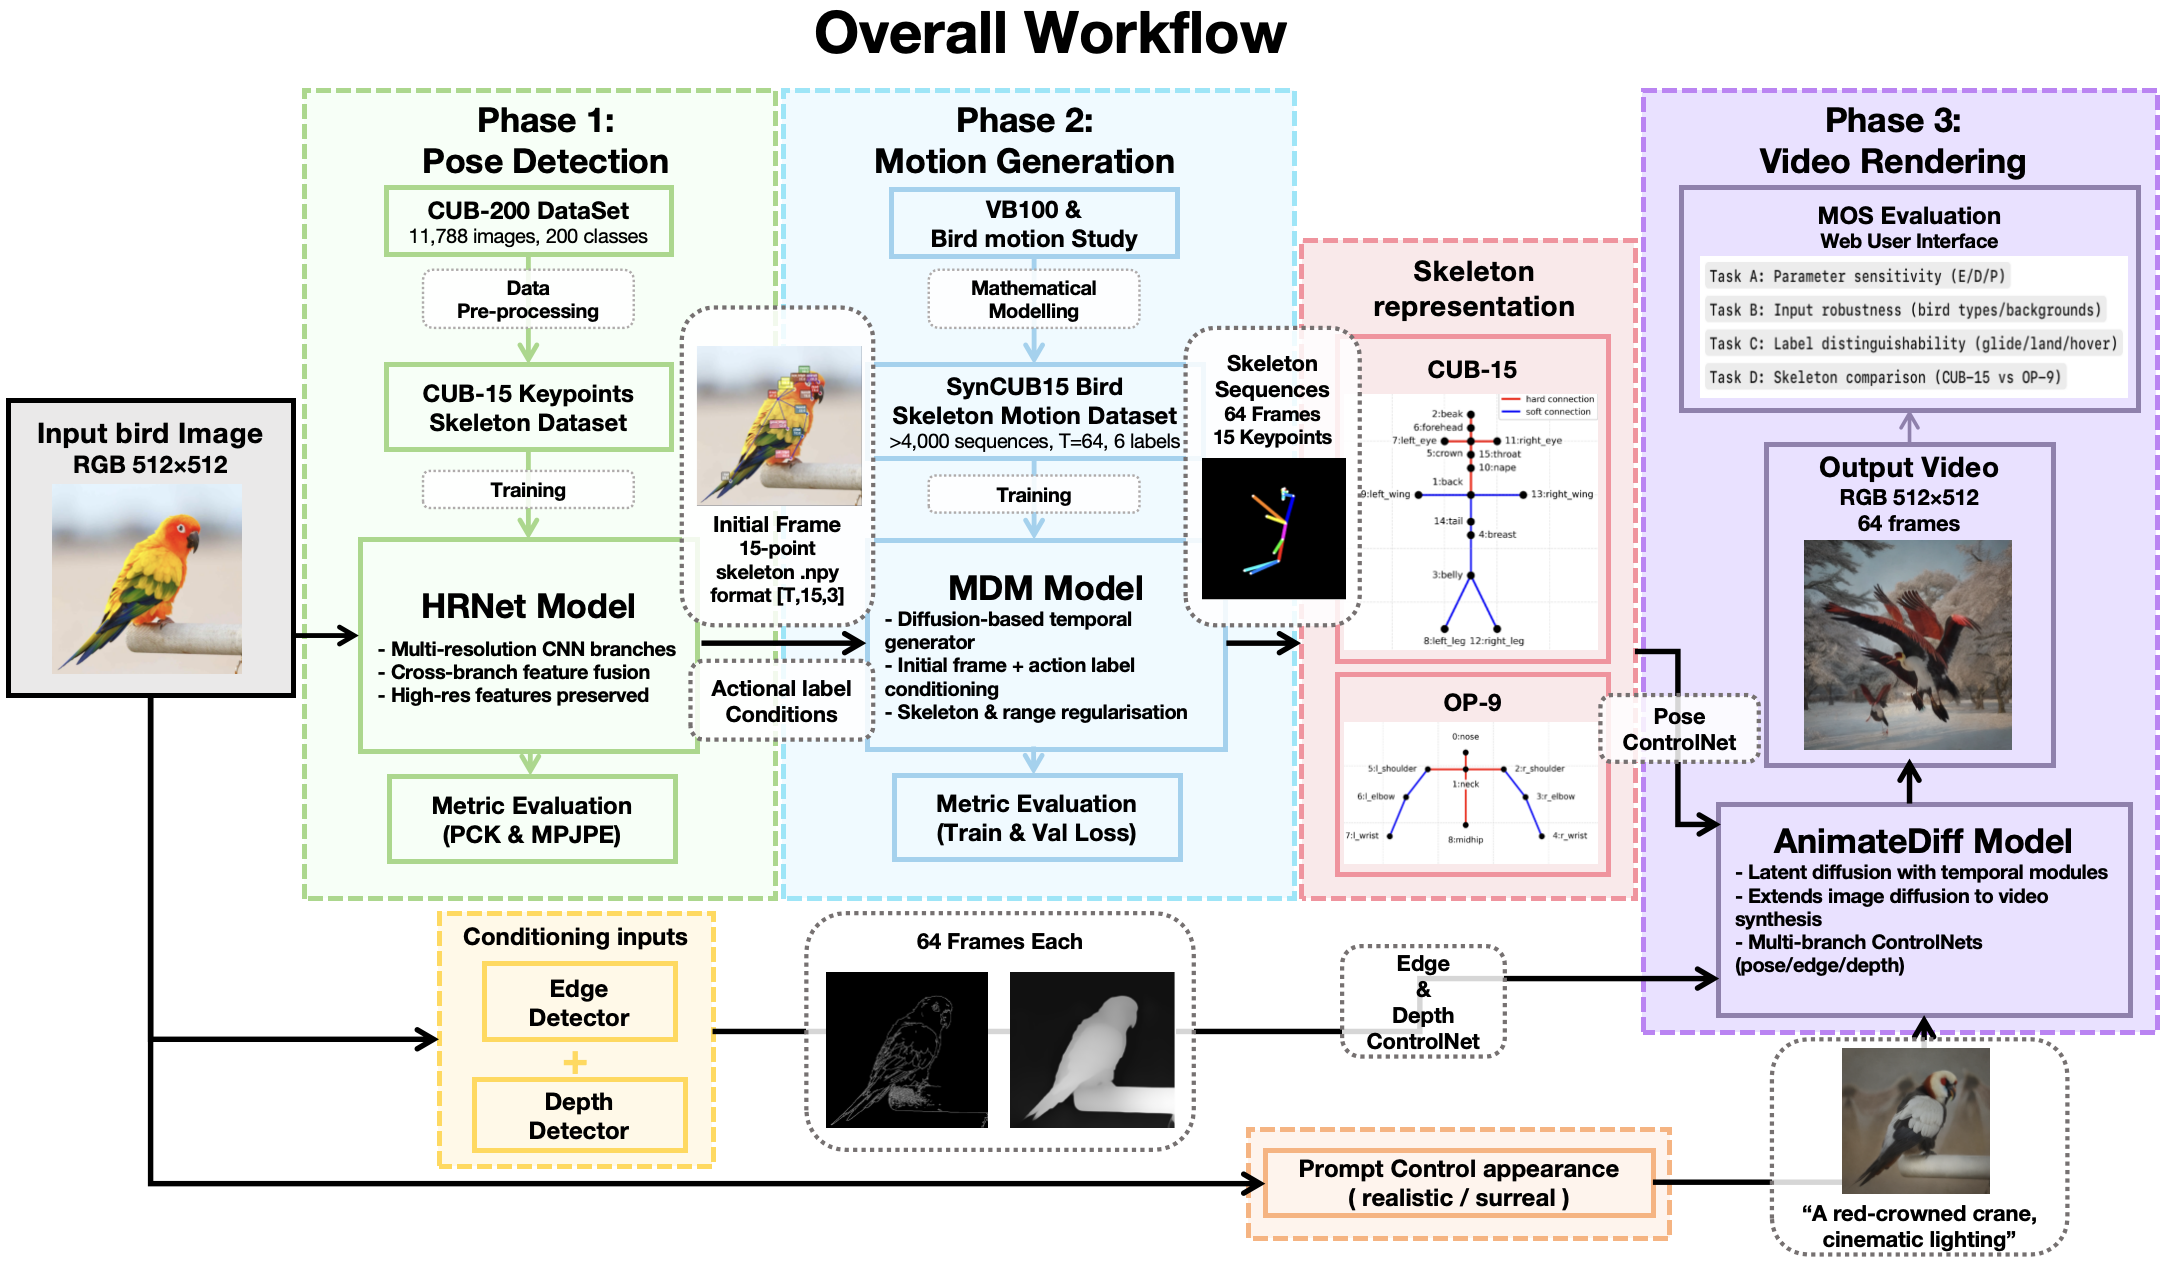
\includegraphics[width=\textwidth]{figures/Workflow.png}
    \caption{Overall workflow of the proposed Dreambirds pipeline.}
    \label{fig:workflow}
\end{figure}


% \begin{figure}[t]
% \centering
% \resizebox{\linewidth}{!}{%
% \begin{tikzpicture}[
%   font=\small,
%   node distance=8mm and 10mm,
%   >=Latex,
%   block/.style={rounded corners, draw, thick, align=center, fill=white, minimum height=6mm},
%   titleb/.style={rounded corners, draw, thick, align=center, fill=gray!15, inner sep=2pt},
%   group/.style={rounded corners, draw, ultra thick, inner sep=4pt, fill=yellow!8},
%   line/.style={-Latex, thick},
%   annot/.style={align=left}
% ]

% % -------- TRAINING --------
% \node[group, minimum width=11.8cm, minimum height=4.8cm, label={[annot]above:{\textbf{Training}}}] (trainbox) {};
% \node[block, fill=blue!10]  (cub200)  at ([xshift=-4.5cm,yshift=1.6cm]trainbox.center) {CUB-200\\Bird Image Dataset};
% \node[block, fill=blue!10, below=of cub200] (preproc) {Data Preprocessing\\$\rightarrow$ CUB-15 dataset\\with skeletons};
% \node[block, fill=blue!10, below=of preproc] (hrnet) {HRNet\\(keypoint detector)};

% \node[block, fill=green!10] (vb100)   at ([xshift=3.7cm,yshift=1.6cm]trainbox.center) {VB100$+$\\Bird motion papers};
% \node[block, fill=green!10, below=of vb100] (synset) {Mathematical modelling\\$\rightarrow$ SynCUB15\\Bird Skeleton Motion Dataset};
% \node[block, fill=green!10, below=of synset] (mdm)   {MDM\\(motion diffusion)};

% \node[block, fill=orange!12] (prepctrl) at ([xshift=0cm,yshift=-1.0cm]trainbox.south) {Prepare control branches:\\Edge \& Depth detectors};

% % -------- GENERATING --------
% \node[group, minimum width=11.8cm, minimum height=5.4cm, below=16mm of trainbox, label={[annot]below:{\textbf{Generating}}}] (genbox) {};

% \node[block, fill=white]                      (inputimg)  at ([xshift=-5.0cm,yshift=0.8cm]genbox.center) {Input Bird Image};
% \node[block, fill=white, below=8mm of inputimg] (appear)    {Appearance conditioning:\\Input image $+$ text prompt};

% \node[block, fill=white, right=15mm of inputimg] (hrnet_gen) {Pose detection\\(HRNet $\rightarrow$ CUB-15)};
% \node[block, fill=white, below=8mm of hrnet_gen] (staticnp)  {CUB-15 skeleton\\(single-frame keypoints)};
% \node[block, fill=white, right=20mm of hrnet_gen, yshift=6mm] (mdm_gen) {Skeleton motion sequence\\$[T,15,3]$ $+$ action labels};
% \node[block, fill=white, below=8mm of mdm_gen] (poserender) {Pose Renderer\\$\rightarrow$ Pose PNG\\(CUB-15 / OP-9)};

% \node[block, fill=white, right=18mm of staticnp] (edgen) {Canny Edge \& Depth PNG};

% \node[block, fill=white, right=20mm of poserender, yshift=6mm, minimum width=24mm, minimum height=12mm] (ad) {AnimateDiff\\$+$ ControlNet\\(pose, edge, depth)};
% \node[block, fill=white, right=14mm of ad] (outvid) {Output Video};

% % connections
% \draw[line] (cub200) -- (preproc);
% \draw[line] (preproc) -- (hrnet);
% \draw[line] (vb100) -- (synset);
% \draw[line] (synset) -- (mdm);

% \draw[dashed, line] (hrnet.south) -- ++(0,-0.7) -| (hrnet_gen.north);
% \draw[dashed, line] (mdm.south) -- ++(0,-0.7) -| (mdm_gen.north);
% \draw[dashed, line] (prepctrl.south) -- ++(0,-0.3) -| (edgen.north);

% \draw[line] (inputimg) -- (hrnet_gen);
% \draw[line] (hrnet_gen) -- (staticnp);
% \draw[line] (staticnp) -- (edgen);
% \draw[line] (mdm_gen) -- (poserender);
% \draw[line] (poserender) -- (ad);
% \draw[line] (edgen) |- (ad);
% \draw[line] (appear) -| (ad);
% \draw[line] (ad) -- (outvid);

% \draw[line] (inputimg) -- (appear);
% \draw[line] (hrnet_gen.east) -- ++(0.5,0) |- (mdm_gen.west);

% \node[annot, align=left] at ([xshift=-3.8cm,yshift=-2.0cm]genbox.south) {Pose branch: per-frame Pose PNG (CUB-15 / OP-9)};
% \node[annot, align=left] at ([xshift=2.2cm,yshift=-2.0cm]genbox.south)  {Edge/Depth branches: static priors};

% \end{tikzpicture}%
% }
% \caption{Workflow of the proposed three-stage pipeline. Training: HRNet on CUB-200 and MDM on a procedurally constructed SynCUB15 motion set; edge/depth control branches are prepared. Generating: HRNet yields CUB-15 keypoints; MDM outputs a motion sequence $[T,15,3]$; a Pose Renderer produces Pose PNGs (CUB-15 or OP-9). AnimateDiff with ControlNet (pose, edge, depth) renders the final video with appearance conditioning.}
% \label{fig:workflow_birds}
% \end{figure}

\newpage

\subsection{Dataset}
\subsubsection{CUB dataset} \label{sec:cubdataset}
% The Caltech-UCSD Birds-200-2011 (CUB-200-2011) dataset contains 11,788 images across 200 bird species with 15 manually annotated part locations (beak, crown, wings, legs, tail). However, these keypoints lack structural connectivity, making them unsuitable for motion modeling. We designed a custom skeleton schema (shown in Fig \ref{fig:top_frame}) connecting the 15 landmarks through:

% \textbf{Rigid connections}: anatomically stable links (beak–crown–nape–back spine, crown–forehead–throat, crown–left/right eye)

% \textbf{Flexible connections}: variable appendages (back–left/right wing, back–tail, belly–left/right leg)

% This transforms scattered keypoints into a coherent skeletal graph encoded in \texttt{skeleton.yaml} format. The design balances anatomical plausibility with motion modelling flexibility, ensuring compatibility with ControlNet-based rendering. A data preparation pipeline converts raw annotations into COCO-style format by parsing \texttt{partlocs.txt} into $15\times 3$ arrays, embedding skeleton connections, calculating bounding boxes, validating data quality, and outputting standardized COCO JSON format. This creates a structured 15-point skeleton dataset compatible with pose estimation frameworks. 

% The restructured skeleton not only enables HRNet training, but also provides a quantitative basis for evaluation. Specifically, the annotated skeletons serve as ground truth for PCK and MPJPE metrics when assessing detection accuracy. Figure~\ref{fig:frame4} illustrates the custom CUB-15 skeleton schema and pre-processed CUB-200 dataset images with annotated keypoints and connections, which form the input for HRNet training.



The Caltech-UCSD Birds-200-2011 (CUB-200-2011) dataset contains 11,788 images across 200 bird species with 15 manually annotated part locations (beak, crown, wings, legs, tail). However, these keypoints lack structural connectivity, making them unsuitable for motion modelling. We therefore designed a custom 15-point skeleton schema (Fig.~\ref{fig:top_frame}) that links rigid anatomical parts (e.g., beak–crown–nape–back spine) and flexible appendages (e.g., back–wings, back–tail, belly–legs) into a coherent graph encoded in \texttt{skeleton.yaml}.  

The annotations were converted into COCO-style format through a preprocessing pipeline, creating a structured dataset compatible with standard pose estimation frameworks. This restructured skeleton not only enabled HRNet training, but also provided a quantitative basis for evaluation using PCK and MPJPE metrics. Figure~\ref{fig:frame4} illustrates the custom skeleton schema and example annotated images, which serve as input for HRNet training.  


\begin{figure}[H]
    \centering

    % -------- Row 1: single, centered --------
    \begin{subfigure}[t]{0.3\textwidth}
        \centering
        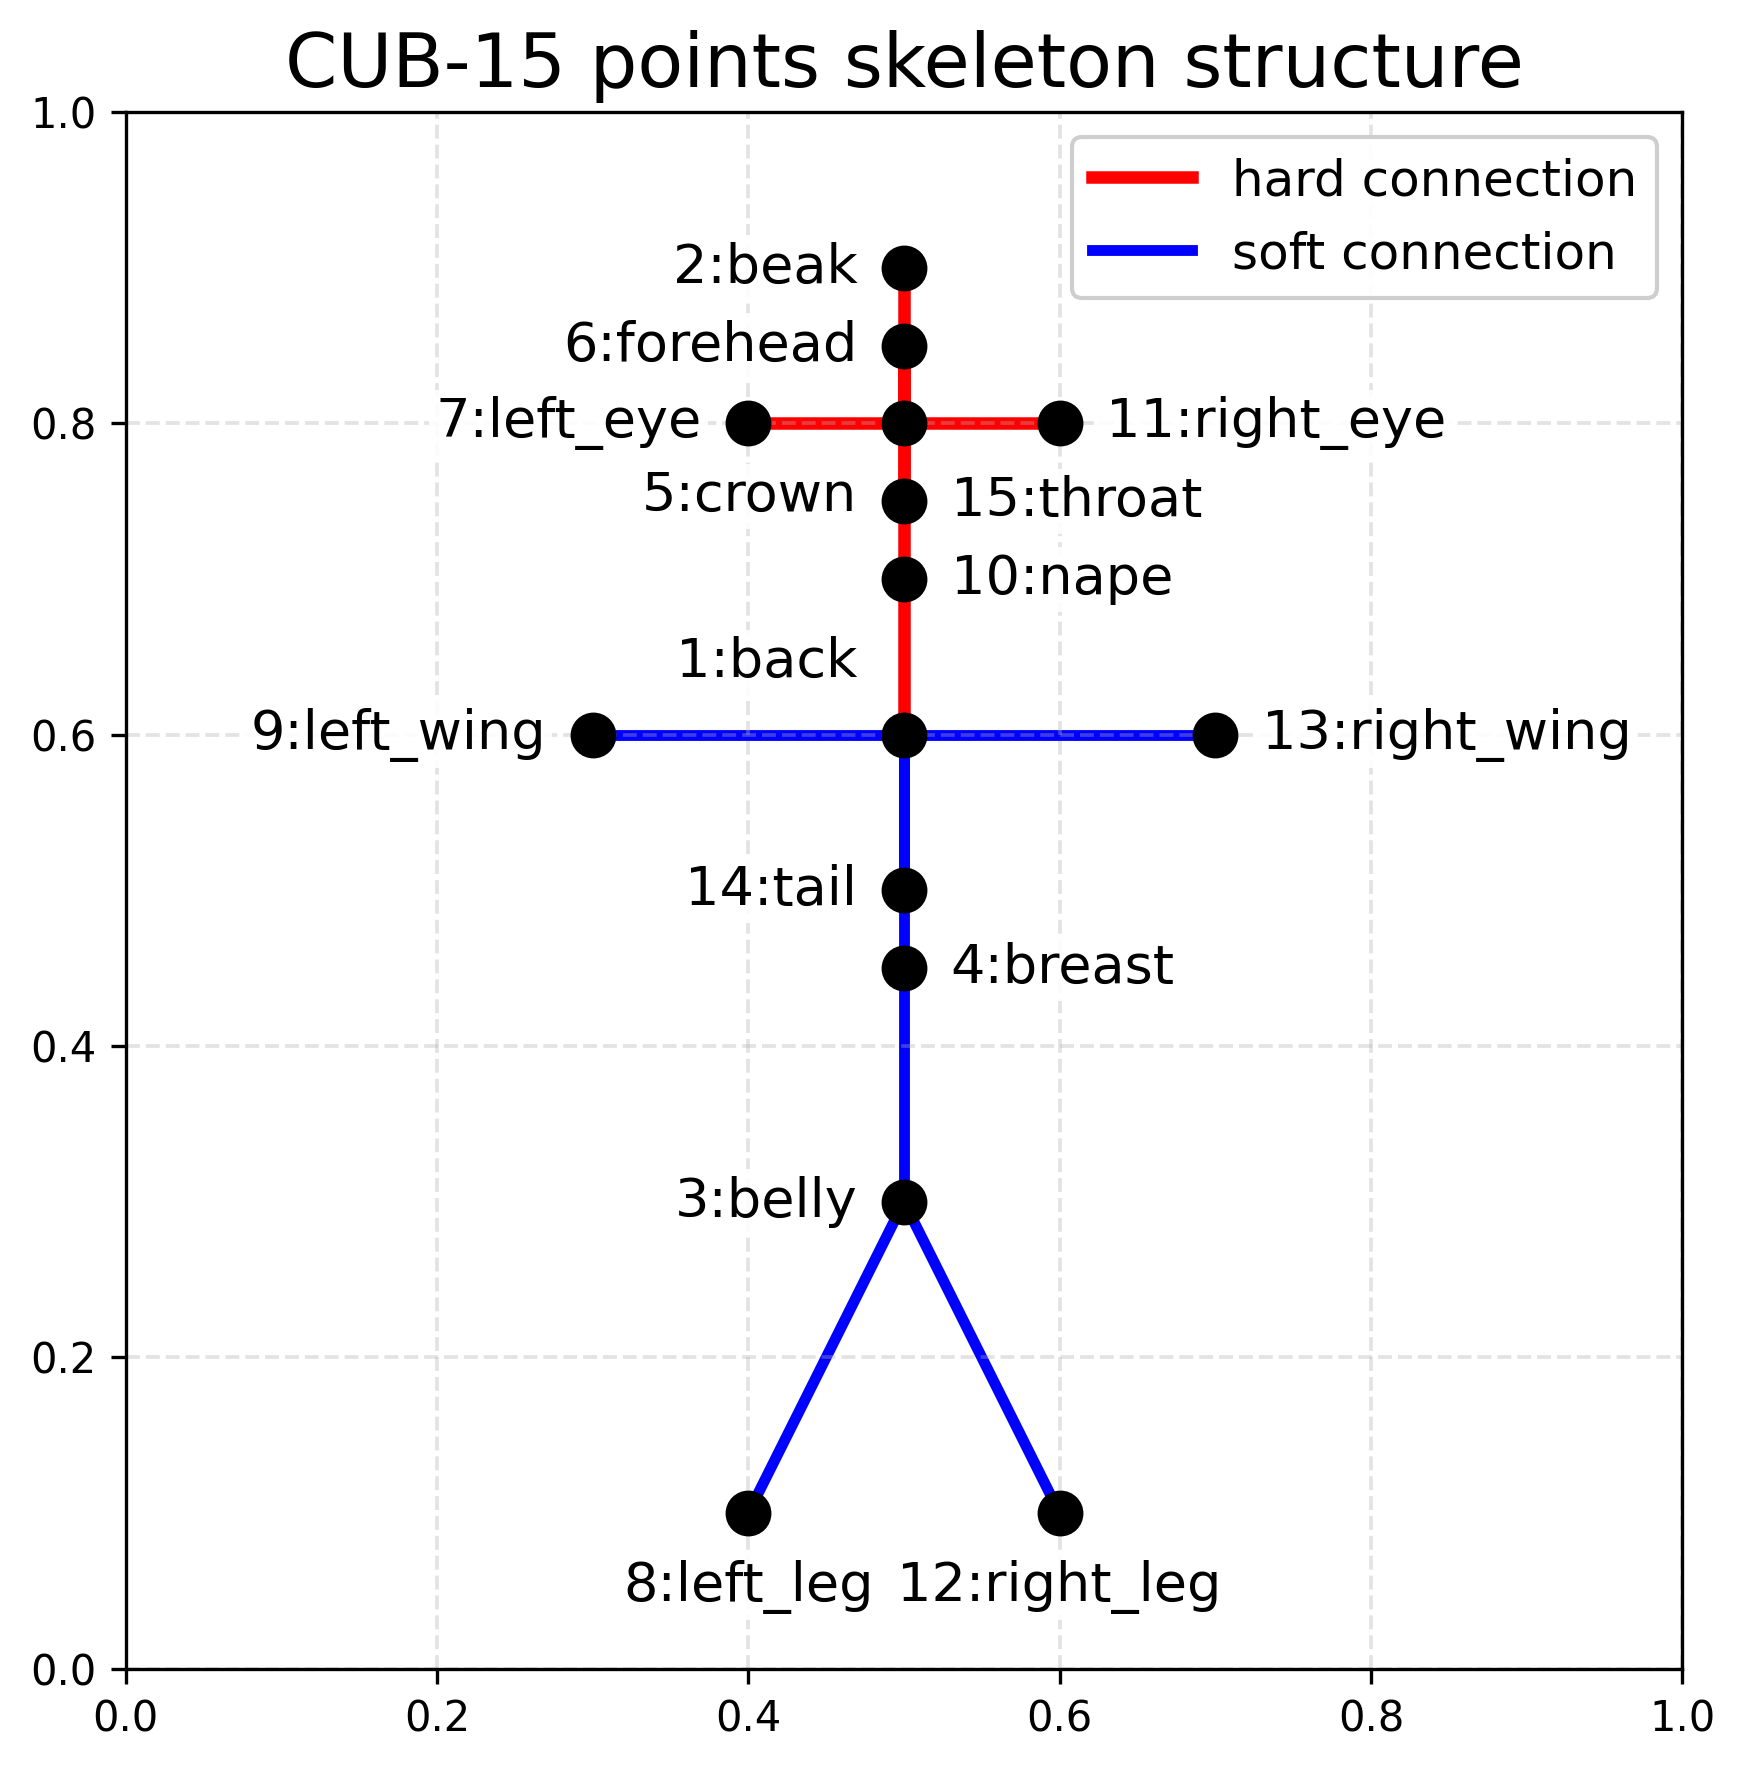
\includegraphics[width=\textwidth]{figures/ReportFigures/skeleton_structure.png}
        \caption{}
        \label{fig:top_frame}
    \end{subfigure}

    \vspace{0.8em}

    % -------- Row 2: three side-by-side, centered as a group --------
    \begin{minipage}{0.80\textwidth} % 控制整行宽度以便居中
        \centering
        \begin{subfigure}[t]{0.30\textwidth}
            \centering
            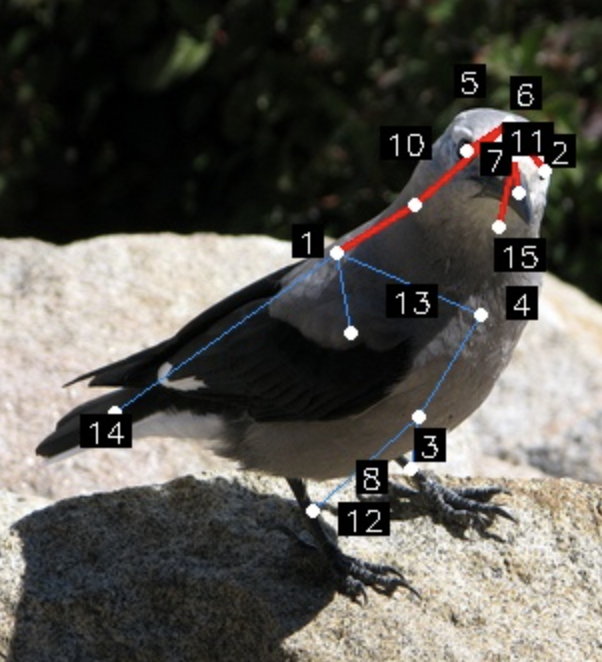
\includegraphics[height=4cm,keepaspectratio]{figures/ReportFigures/Fig3-1.png}
            % \label{fig:frame3}
        \end{subfigure}\hfill
        \begin{subfigure}[t]{0.30\textwidth}
            \centering
            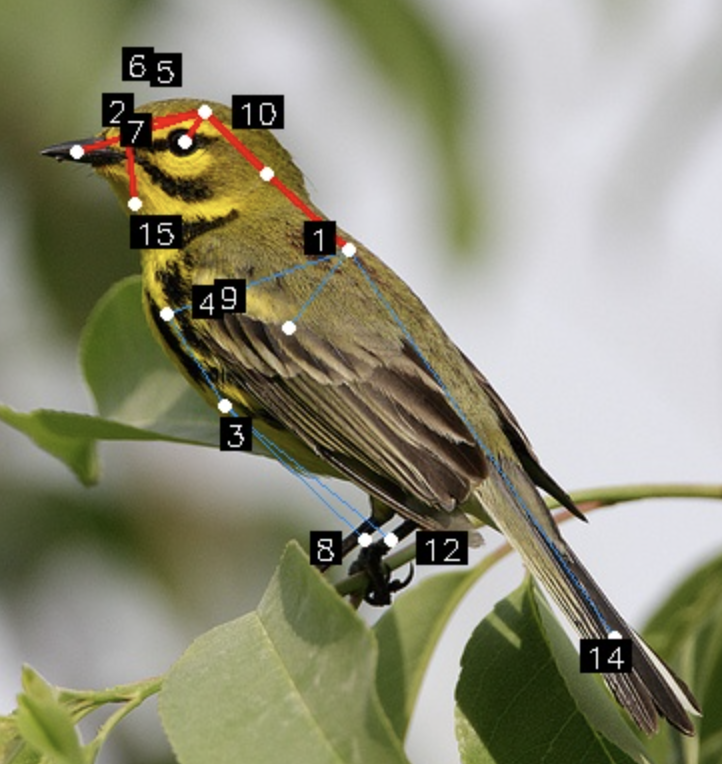
\includegraphics[height=4cm,keepaspectratio]{figures/ReportFigures/Fig3-2.png}
            \caption{}
            \label{fig:frame4}
        \end{subfigure}\hfill
        \begin{subfigure}[t]{0.30\textwidth}
            \centering
            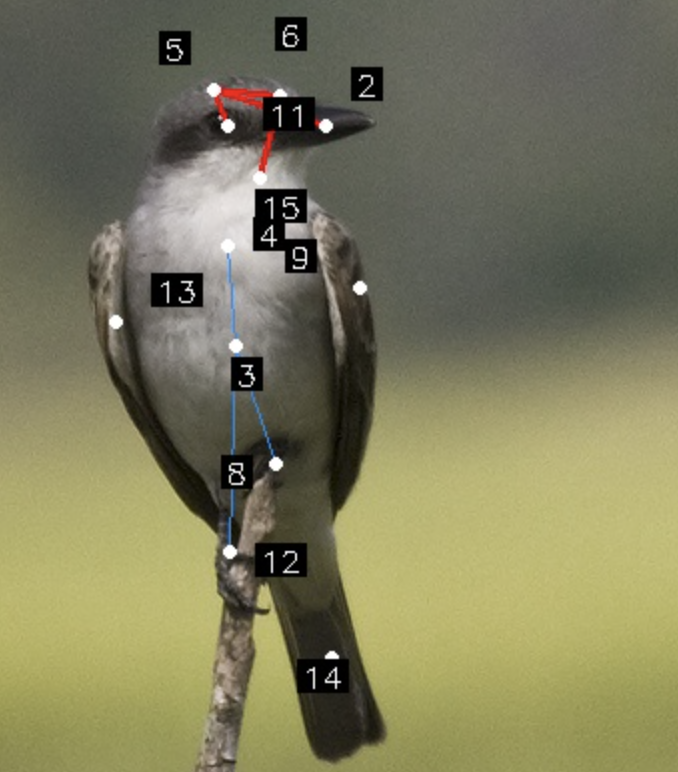
\includegraphics[height=4cm,keepaspectratio]{figures/ReportFigures/Fig3-3.png}
            % \label{fig:frame5}
        \end{subfigure}
    \end{minipage}

    \caption{(a) Visualisation of the custom CUB-15 skeleton structure, with rigid (red) and flexible (blue) connections.
    (b) Pre-processed CUB-200 dataset images with annotated keypoints and skeletal connections, used as input for HRNet training.}
    \label{fig:frame_comparison_1}
\end{figure}






\subsubsection{SynCUB15 Motion Dataset}
% To address the scarcity of annotated bird motion data, we procedurally generated a synthetic dataset of pose sequences in the format $[T,15,3]$, where 15 anatomical keypoints are represented with three channels per joint (x, y, visibility). Biomechanical constraints such as fixed bone-length ratios and wing-folding limits were imposed to ensure anatomical plausibility. Each sequence thus encodes temporally consistent skeletal dynamics, providing a surrogate for real-world motion capture and serving as training input for the Motion Diffusion Model.

% Each sequence spans 64 frames, capturing the temporal evolution of the head, torso, wings, tail, and legs. To facilitate controllable motion generation, we defined six canonical action categories — takeoff, gliding, hovering, soaring, diving, and landing. These categories were derived from a larger set of fine-grained behavioural phases (covering ground movements, transitional states, and aerial actions) through a canonical mapping scheme. Every sequence was assigned a primary label from this taxonomy, which later serves as the conditioning signal for Motion Diffusion Model training. In addition, initial-pose conditioning can be applied by anchoring the first frame to a detected skeleton, ensuring stable sampling during inference.

% The dataset was generated with a biomechanics-inspired model that integrates species-specific parameters such as wingspan, body length, flapping frequency, and agility, along with environmental effects including wind speed and turbulence. Anatomical constraints on bone length and joint angles were applied to preserve biological realism. To further enhance diversity, we employed data augmentation techniques including temporal warping, spatial scaling and rotation, mirroring, and controlled noise injection. These augmentations not only increased variability but also mitigated overfitting, ensuring that the Motion Diffusion Model generalises to unseen skeleton configurations.

% In total, the corpus contains more than 4,000 labelled sequences, stratified into training and validation subsets, enabling the Motion Diffusion Model to learn species-aware, biomechanically grounded transitions. The VB100 video dataset was additionally used as a qualitative reference for assessing motion realism and informing the behavioural taxonomy. VB100 clips were not directly used for training, but provided guidance for evaluating motion plausibility and ensuring that the taxonomy reflects common flight actions and natural variation. Overall, the dataset offers a scalable and balanced alternative to scarce real-world motion data, supporting conditional training of Motion Diffusion Models for controllable bird motion generation. 
To address the scarcity of annotated bird motion data, we procedurally generated a synthetic dataset of pose sequences in the format $[T, 15, 3]$, where 15 anatomical keypoints are represented with $(x, y, \text{visibility})$. Biomechanical constraints such as fixed bone-length ratios and wing-folding limits were imposed to ensure anatomical plausibility. Each sequence thus encodes temporally consistent skeletal dynamics, serving as a surrogate for real-world motion capture and as training input for the Motion Diffusion Model (MDM).  

Each sequence spans 64 frames, capturing the temporal evolution of the head, torso, wings, tail, and legs. To enable controllable motion generation, we defined six canonical action categories—takeoff, gliding, hovering, soaring, diving, and landing—derived from a broader behavioural taxonomy. Each sequence was assigned a label from this taxonomy, later used as conditioning input for MDM training. Inference stability was further supported by anchoring the first frame to a detected skeleton.  Biomechanical constraints and augmentation strategies were used to ensure realism and diversity, enhancing dataset variability and mitigating overfitting.  

In total, the corpus contains over 4,000 labelled sequences, stratified into training and validation subsets, enabling MDM to learn species-aware, biomechanically grounded transitions. The VB100 dataset was additionally used as a qualitative reference for evaluating motion plausibility and informing the taxonomy, ensuring the dataset reflects common flight actions and natural variation. Overall, SynCUB15 provides a scalable surrogate for real-world motion capture, supporting MDM training for controllable bird motion generation. Figure~\ref{fig:frame_comparison_2} shows sample frames of SynCUB15 skeleton sequences.


\begin{figure}[htbp]
    \centering

    \begin{subfigure}[t]{0.23\textwidth}
        \centering
        \includegraphics[width=\textwidth]{figures/ReportFigures/Fig2-1.png}
        % \caption{}
        \label{fig:gen_frame1}
    \end{subfigure}\hfill
    \begin{subfigure}[t]{0.23\textwidth}
        \centering
        \includegraphics[width=\textwidth]{figures/ReportFigures/Fig2-2.png}
        % \caption{}
        \label{fig:gen_frame2}
    \end{subfigure}\hfill
    \begin{subfigure}[t]{0.23\textwidth}
        \centering
        \includegraphics[width=\textwidth]{figures/ReportFigures/Fig2-3.png}
        % \caption{}
        \label{fig:gen_frame3}
    \end{subfigure}\hfill
    \begin{subfigure}[t]{0.23\textwidth}
        \centering
        \includegraphics[width=\textwidth]{figures/ReportFigures/Fig2-4.png}
        % \caption{}
        \label{fig:gen_frame4}
    \end{subfigure}

    \caption{Sample frames front-view (XY) projections of CUB-15 skeleton sequences used for Motion Diffusion Model training.}
    \label{fig:frame_comparison_2}
\end{figure}


% \subsubsection{Surreal Bird Dataset}
% A collection of surreal bird images created by Ziqi Yue using ChatGPT API provides visual guides for appearance prompt engineering. These stylized images depict birds with anthropomorphic clothing, accessories, and poses, serving as inspiration for aligning motion dynamics with surreal aesthetics in final video synthesis. While not used as training data, they ensure coherence between motion features and artistic intent.



\subsection{Keypoint Detection using HRnet}

% Building on the restructured CUB-15 dataset (Section~2.2.1), the first stage requires a reliable pose detector for extracting structured skeletons from bird images. Since downstream motion generation and video synthesis depend on temporally consistent sequences, accurate localisation of both rigid anatomical landmarks (beak, crown, back, tail) and flexible appendages (wings, legs) is essential.

% We used the preprocessed CUB dataset in \ref{sec:cubdataset}. High-Resolution Network (HRNet-W32) was selected for its ability to maintain high-resolution representations throughout the network, enabling precise localisation of fine-scale details. Unlike traditional CNNs that progressively downsample, HRNet’s design suits the fine-grained keypoint detection required for bird skeleton estimation. This is particularly advantageous for small anatomical parts such as eyes and beak, which are critical for orientation cues in later skeleton-conditioned rendering. Implementation used the MMPose framework with an input resolution of $256\times256$ and a $64\times64$ heatmap output for 15 keypoint channels. 
% % We used the preprocessed CUB dataset in \ref{sec:cubdataset}.
% % % Model Architecture: 
% % High-Resolution Network (HRNet-W32) was selected for its ability to maintain high-resolution representations throughout the network, enabling precise localisation of fine-scale details. Unlike traditional CNNs that progressively downsample, HRNet's design suits the fine-grained keypoint detection required for bird skeleton estimation.
% % % Training Setup: 
% % Implementation used the MMPose framework with an input resolution of \(256\times 256\) and a \(64\times 64\) heatmap output for 15 keypoint channels.
% Training employed the AdamW optimizer (learning rate \(1\times 10^{-4}\), weight decay \(0.01\)) with linear warm-up and multi-step decay.
% Data augmentation included horizontal flipping, affine transformations, and rotations.

% % The model was trained on 5{,}000 images for 50 epochs.

% % \textbf{Evaluation metrics.} 
% We evaluate HRNet-W32 on the CUB-15 validation set using Percentage of Correct Keypoints (PCK) and normalized localization error. A prediction for keypoint $i$ is counted correct if $\|\hat{p_i} - p_i\|_2/\sqrt{w^2+h^2} \leq \tau$, where $w, h$ are the ground-truth bounding-box width and height; we report overall and per-keypoint PCK at $\tau \in \{0.05,0.10,0.15,0.20\}$ using only visible keypoints. To analyze articulation, we also group landmarks and report PCK@0.1 for \textbf{rigid vs.~flexible} parts, consistent with the skeleton design in Section~2.2.1. For paired structures (wings, legs), left–right confusion is flagged when the predicted left/right pair distance is $<0.1$ of the bounding-box diagonal, and we report the confusion rate. Finally, normalized error is summarized as the mean $\pm$ std of the above distance per keypoint to complement PCK.


% % \subsection{Evaluation Metrics}
% We evaluate HRNet-W32 on the CUB-15 validation set using \textbf{Percentage of Correct Keypoints (PCK)} and normalized localization error.

% \paragraph{PCK.}
% A prediction for keypoint $i$ is correct if
% \[
% \frac{\lVert \hat{\mathbf{p}}_i - \mathbf{p}_i \rVert_2}{\sqrt{w^2 + h^2}} \le \tau,
% \]
% where $w,h$ are the ground-truth bounding-box width and height. We report overall and per-keypoint PCK at $\tau \in \{0.05, 0.10, 0.15, 0.20\}$, using only visible keypoints.

% \paragraph{Per-keypoint and grouped PCK.}
% Beyond per-keypoint PCK@0.1, landmarks are grouped into \emph{rigid} and \emph{flexible} parts to assess articulated difficulty.

% \paragraph{Left--Right confusion.}
% For paired parts (wings, legs), we flag confusion if the predicted left/right pair distance is $<0.1$ times the bbox diagonal, and report confusion rates.

% \paragraph{Normalized error.}
% We summarize mean $\pm$ std of the normalized distance per keypoint to capture variance complementary to PCK.

%%%%%%%%%%%%%%%%%%%%%%%%%%%%%%
% Building on the restructured CUB-15 dataset (Section \ref{sec:cubdataset}), the first stage requires a reliable pose detector for extracting structured skeletons from bird images. Since downstream motion generation and video synthesis depend on temporally consistent sequences, accurate localisation of both rigid anatomical landmarks (beak, crown, back, tail) and flexible appendages (wings, legs) is essential.

% We adopt the High-Resolution Network (HRNet-W32) for its ability to maintain high-resolution representations throughout the network, enabling precise localisation of fine-scale details. Unlike conventional CNNs that progressively downsample, HRNet preserves high-resolution feature maps, which is advantageous for detecting small anatomical structures such as eyes and beak. Implementation is based on the MMPose framework, with input images resized to $256\times256$ and output heatmaps of $64\times64$ for 15 keypoints.

% Training was performed on 5,000 images for 50 epochs using the AdamW optimizer with a learning rate of $1\times10^{-4}$, weight decay of 0.01, linear warm-up, and multi-step decay. To improve generalisation, we applied data augmentation including horizontal flipping, affine transformations, and random rotations. 

% The trained HRNet is evaluated on the CUB-15 validation set. Evaluation criteria include Percentage of Correct Keypoints (PCK) and Mean Per-Joint Position Error (MPJPE). Results are reported both per keypoint and grouped into rigid vs.\ flexible categories, consistent with the skeleton definition in Section \ref{sec:cubdataset}. 




Building on the restructured CUB-15 dataset (Section~\ref{sec:cubdataset}), the first stage requires a reliable pose detector for extracting structured skeletons from bird images. Since downstream motion generation and video synthesis depend on temporally consistent sequences, accurate localisation of both rigid anatomical landmarks (beak, crown, back, tail) and flexible appendages (wings, legs) is essential.  

We adopt the High-Resolution Network (HRNet-W32) for its ability to maintain high-resolution representations throughout the network, enabling precise localisation of fine-scale details. Unlike conventional CNNs that progressively downsample, HRNet preserves high-resolution feature maps, which is advantageous for detecting small anatomical structures such as eyes and beak. Implementation is based on the MMPose framework, with input images resized to $256 \times 256$ and output heatmaps of $64 \times 64$ for 15 keypoints.  

The trained HRNet is evaluated on the CUB-15 validation set. 
% Evaluation criteria include Percentage of Correct Keypoints (PCK) and Mean Per-Joint Position Error (MPJPE). 
Results are reported both per keypoint and grouped into rigid vs. flexible categories, consistent with the skeleton definition in Section~\ref{sec:cubdataset}.



\subsection{Pose Sequence Generation using MDM}

% The motion module transforms static bird skeletons into temporally coherent pose sequences. While CUB dataset provides only still-image annotations, downstream video synthesis requires dynamic trajectories with species-aware movements and biomechanically plausible transitions. 

% We employ the Motion Diffusion Model (MDM), a generative framework capturing motion variability while preserving temporal smoothness. MDM combines the generative capacity of diffusion models with the sequential modelling power of Transformers, enabling the synthesis of smooth and diverse motion trajectories. The model learns to denoise skeleton sequences from Gaussian noise through iterative refinement, which makes it particularly effective for capturing long-range temporal dependencies compared to recurrent or adversarial approaches.


% % \textbf{Training objectives.} 
% The model is trained on 64-frame sequences in the format $[T,15,3]$, with six canonical action labels (takeoff, gliding, hovering, soaring, diving, landing) serving as conditioning signals. The objective follows the standard diffusion denoising formulation, supplemented by additional constraints to ensure anatomical and temporal stability:
% \begin{enumerate}
%     \item Denoising loss: reconstruct clean motion from noisy inputs.
%     \item Skeletal constraints: enforce fixed bone lengths and anatomical plausibility.
%     \item Coordinate regularisation: restrict predictions to valid spatial ranges.
%     \item Initial-frame consistency: encourage generated sequences to remain aligned with the ground-truth first frame.
% \end{enumerate}

% % \textbf{Inference procedure.}
% At inference, the model is conditioned on an initial skeleton frame and an action label. Generation proceeds by iterative denoising with classifier-free guidance, while softly anchoring the first few frames to the user-provided pose. The final output is a 64-frame skeleton sequence that adheres to the chosen action label and evolves smoothly from the initial posture, enabling controllable bird motion generation.

% The resulting MDM outputs serve as motion blueprints for the rendering stage, providing temporally consistent trajectories suitable for skeleton-conditioned video synthesis.


The motion module transforms static bird skeletons into temporally coherent pose sequences. While the CUB dataset provides only still-image annotations, downstream video synthesis requires dynamic trajectories with species-aware movements and biomechanically plausible transitions.  

We employ the Motion Diffusion Model (MDM), a generative framework that captures motion variability while preserving temporal smoothness. MDM combines the generative capacity of diffusion models with the sequential modelling power of Transformers, enabling the synthesis of smooth and diverse motion trajectories. The model learns to denoise skeleton sequences from Gaussian noise through iterative refinement, which makes it particularly effective for capturing long-range temporal dependencies compared to recurrent or adversarial approaches.  

The model is trained on 64-frame sequences with six canonical action labels (takeoff, gliding, hovering, soaring, diving, landing) serving as conditioning signals. The objective follows the standard diffusion denoising formulation, supplemented by additional constraints to ensure anatomical plausibility and temporal stability. These include fixed bone lengths, spatial validity, and alignment with the ground-truth initial frame.  

At inference, the model is conditioned on an initial skeleton frame and an action label. Generation proceeds by iterative denoising with classifier-free guidance, while softly anchoring the first frames to the user-provided pose. The final output is a 64-frame skeleton sequence that adheres to the chosen action label and evolves smoothly from the initial posture, enabling controllable bird motion generation.  

The resulting MDM outputs serve as motion blueprints for the rendering stage, providing temporally consistent trajectories suitable for skeleton-conditioned video synthesis.




\subsection{Video Generation using AnimateDiffusion+ ControlNet}

% The objective of this stage is to generate temporally coherent bird videos that follow skeleton-driven motion while maintaining consistent appearance and volumetric structure. To achieve this, we employ AnimateDiff for temporal modelling, combined with multiple ControlNets that inject complementary constraints into the diffusion process.

% AnimateDiff extends Stable Diffusion with a Motion Adapter, introducing lightweight temporal consistency across frames. ControlNet augments the model by conditioning generation on external structural maps, with multiple branches fused into the denoising network to allow simultaneous control of shape, depth, and motion. AnimateDiff introduces temporal coherence through a modular Motion Adapter integrated with ControlNet-conditioned models. The Motion Module inserts temporal self-attention layers and 1D temporal convolutions between existing UNet spatial layers. Multi-ControlNet integration processes three conditioning signals (Canny, Depth, OpenPose) through parallel encoder branches, injecting features via zero-initialized convolutions at corresponding decoder stages. Static conditions provide structural constraints across frames while dynamic skeleton poses guide frame-specific motion.
% Three complementary conditioning signals were adopted:
% \begin{enumerate}
%     \item Canny edges (global silhouette): preserve contours and prevent drifting.
%     \item Depth maps (volumetric structure): provide coarse 3D cues for realism.
%     \item OpenPose-style skeletons (pose/motion): derived from input skeleton sequences, ensuring frame-level kinematic consistency.
% \end{enumerate}
% Canny and depth maps are repeated as static priors across frames, while per-frame skeleton renders provide dynamic motion control. The relative influence of each branch is tuned via scale factors; higher skeleton weights enforce motion fidelity at the cost of visual flexibility.

% We validate and normalise skeleton .npy sequences and rescale them to the target canvas, render per-frame pose PNGs suitable for ControlNet (with normalisation, resampling, and visibility handling), extract Canny edges and depth from reference images as static priors replicated across frames, run inference with SD-1.5 + AnimateDiff Motion Adapter and three ControlNets by feeding [Canny, Depth, Pose] to a standard sampler, and export PNG frames and assemble GIF/MP4 while logging seeds/configs for reproducibility; all conditioning inputs are resolution-aligned (Canny/Depth in grayscale or RGB, Pose as per-frame PNG), Pose is provided at every timestep while Canny/Depth are reused across frames, consistent keypoint ordering prevents topology errors, and mixed precision (FP16) is preferred since memory scales roughly linearly with resolution × frame count.

% We use a manually recorded Mean Opinion Score procedure, as a complement to objective metrics, to assess generated bird videos on five aspects: \emph{motion fidelity to skeleton} (1 = clearly off-skeleton, 5 = strictly follows), \emph{temporal smoothness} (1 = stutter/flicker, 5 = smooth), \emph{appearance consistency} (1 = drifting/broken, 5 = stable), \emph{surreal trait preservation} (1 = often lost, 5 = well preserved), and an optional \emph{overall quality} score (1 = poor, 5 = excellent). Volunteer raters (\(\geq 5\) recommended), participating anonymously, evaluate clips prepared with unified resolution, frame rate, and duration, alongside the corresponding skeleton sequences. To reduce order bias, clips are presented in a randomized sequence. Raters watch each clip in full and assign 1--5 scores for the five dimensions, with optional brief comments. Scores are recorded manually in a shared spreadsheet (CSV/Excel/Google Sheet) and used for subsequent statistical analysis and visualization.

The objective of this stage is to transform skeleton sequences into temporally coherent videos that preserve surreal traits while maintaining structural fidelity. To this end, we employ AnimateDiff for temporal modelling, combined with multiple ControlNets that provide complementary structural conditions.

AnimateDiff extends Stable Diffusion with a Motion Adapter, introducing temporal consistency across frames. ControlNet augments generation by conditioning on structural maps. Three signals are used: (i) Canny edges, preserving global silhouettes and preventing drift; (ii) depth maps, providing coarse volumetric cues; and (iii) OpenPose-style skeletons (CUB-15/OP-9), enforcing frame-level motion consistency. Together, these modules ensure visual appearance is controlled by static priors, while motion is governed by skeleton inputs.

The workflow proceeds as follows. Skeleton sequences from the Motion Diffusion Model are first smoothed with a Savitzky–Golay filter. The processed \texttt{.npy} files are then converted into OpenPose-style PNGs for ControlNet pose conditioning. Reference images are transformed into multi-frame Canny edge and depth sequences (64 frames), serving as consistent priors. Finally, these three branches (pose, edge, depth) are jointly fed into AnimateDiff, with branch scales tuned to balance motion adherence and appearance fidelity.

Appearance is specified either via textual prompts or directly from the reference image. Prompts introduce surreal traits such as unusual colours or textures, while image conditioning preserves realistic features like plumage and body markings. This dual mechanism allows flexible control between imaginative aesthetics and fidelity to the source bird.

All conditioning inputs are resolution-aligned and normalised. AnimateDiff inference generates frame-by-frame outputs, assembled into GIF or MP4 videos with logged seeds and configurations for reproducibility. The resulting videos achieve controllable motion guided by skeletons, while preserving surreal appearance through prompt conditioning and static edge/depth priors.

% Evaluation of video quality, including both perceptual metrics and human-centred Mean Opinion Scores, is described in Section~2.6.






\subsection{Evaluation}
The evaluation strategy covers all three stages of the pipeline—pose detection, motion generation, and video rendering—ensuring that accuracy, temporal quality, and perceptual fidelity are assessed with complementary criteria. Since the final goal is to produce temporally coherent and stylistically consistent surreal bird motion videos, we employ both objective metrics and human-centred evaluation.

\subsubsection{Pose Detection}
For the HRNet-based detector, evaluation follows standard conventions in pose estimation. We report:

\begin{itemize}
    \item \textbf{PCK (Percentage of Correct Keypoints):} The proportion of detected joints within a normalised error threshold $\tau$ of ground truth. We evaluate at $\tau \in \{0.05,0.10,0.15,0.20\}$, and report results per keypoint as well as grouped into rigid vs.\ flexible categories.
    \item \textbf{MPJPE (Mean Per-Joint Position Error):} The mean Euclidean distance between predicted and ground-truth keypoints (pixels), complementing PCK by capturing localisation error.
    % \item \textbf{Left--right confusion:} For symmetric parts (wings, legs), confusion events are flagged when predictions are swapped across left/right sides. 
\end{itemize}

\subsubsection{Motion Generation}
For the Motion Diffusion Model (MDM), evaluation focuses on the temporal quality and controllability of generated skeleton sequences:
\begin{itemize}
    \item \textbf{Training and validation losses:} We monitor denoising loss, skeletal consistency, coordinate regularisation, and first-frame anchoring loss.
    % \item \textbf{Pose accuracy:} Generated trajectories are compared against validation sequences using PCK and MPJPE, enabling direct comparison with Phase~1.
    \item \textbf{Qualitative error analysis:} Visualisation of skeleton sequences highlights characteristic errors such as wing asymmetry or left--right swaps.
\end{itemize}

\subsubsection{Video Rendering}
% For final video outputs, evaluation emphasises perceptual quality and surreal trait preservation:
% \begin{itemize}
%     \item \textbf{Mean Opinion Score (MOS):} Human raters score generated videos on four criteria (motion fidelity, temporal smoothness, appearance consistency, surreal trait preservation) using a 1--5 Likert scale. Scores are averaged across raters and clips.
% \end{itemize}

% We use a manually recorded Mean Opinion Score procedure, as a complement to objective metrics, to assess generated bird videos on five aspects: 
% \emph{motion fidelity to skeleton} (1 = clearly off-skeleton, 5 = strictly follows), 
% \emph{temporal smoothness} (1 = stutter/flicker, 5 = smooth), 
% \emph{appearance consistency} (1 = drifting/broken, 5 = stable), 
% \emph{surreal trait preservation} (1 = often lost, 5 = well preserved), 
% and an optional \emph{overall quality} score (1 = poor, 5 = excellent). 

% 18 volunteer raters evaluated the clips under unified resolution, frame rate, and duration, with corresponding skeleton sequences as reference. 
% Clips were presented in randomized order to reduce bias, and each rater assigned 1--5 scores for the defined dimensions. 
% Scores were collected in a shared spreadsheet and averaged for analysis.


To complement objective evaluation metrics, we employed a \textbf{Mean Opinion Score (MOS)} procedure to assess the perceptual quality of the generated bird videos. We developed a lightweight web-based interface to facilitate this process: volunteer evaluators could watch randomized clips side-by-side with their corresponding skeleton sequences under unified resolution, frame rate, and duration, and then submit ratings online. 
% This WebUI ensured consistency of presentation, minimized ordering bias, and enabled efficient collection of ratings from 18 evaluators.


Each video was evaluated along four perceptual dimensions using a 1--5 Likert scale: 
\begin{enumerate}
    \item \textbf{Motion fidelity to skeleton}: 1 = clearly off-skeleton, 5 = strictly follows
    \item \textbf{Temporal smoothness}: 1 = stutter or flicker, 5 = smooth
    \item \textbf{Appearance consistency}: 1 = drifting/broken, 5 = stable
    \item \textbf{Surreal trait preservation}: 1 = often lost, 5 = well preserved
\end{enumerate}

An optional \textbf{overall quality} score (1 = poor, 5 = excellent) was also collected in some cases. For each clip, the ratings were averaged across evaluators to obtain the MOS for each dimension, which then served as the basis for subsequent analysis.  

This MOS framework was applied to four experimental settings:
\begin{itemize}
    \item \textbf{Task A Parameter sensitivity}: examining the effect of different parameter values on video quality
    \item \textbf{Task B Input robustness}: evaluating consistency across different bird species, backgrounds, and initial skeletons
    \item \textbf{Task C Label distinguishability}: measuring whether generated clips convey perceivable action labels, quantified primarily by recognition accuracy
    \item \textbf{Task D Skeleton comparison}: comparing CUB-15 versus OP-9 skeletal representations under identical parameters
\end{itemize}

By aggregating ratings across multiple evaluators, the MOS system provides a simple but effective perceptual metric, enabling us to identify optimal parameter ranges, evaluate robustness, verify label controllability, and quantify the influence of skeleton definitions on the generated outputs.





Further details, including the explicit mathematical definitions of all metrics and loss functions, and the screen shot of the MOS WebUI are provided in Appendix~\ref{appendix:evaluation-math} and Appendix ~\ref{appendix: WebUI}.



% The evaluation strategy is designed to cover all three stages of the pipeline, ensuring that skeleton detection, motion generation, and video rendering are assessed with appropriate and complementary criteria. Since the final goal is to generate temporally coherent and stylistically consistent surreal bird motion videos, both objective metrics and human-centred evaluation are employed.

% \subsubsection{Pose Detection (Phase 1)}
% For the HRNet-based detector, evaluation follows conventions in pose estimation. 
% \begin{itemize}
%     \item \textbf{PCK (Percentage of Correct Keypoints)}: Computed at multiple thresholds (e.g., PCK@0.05, PCK@0.1) to measure the proportion of detected keypoints falling within a tolerance relative to ground-truth annotations. Results are reported per keypoint, grouped into rigid vs.\ flexible parts, and aggregated across the dataset.
%     \item \textbf{MPJPE (Mean Per-Joint Position Error)}: The mean Euclidean distance between predicted and ground-truth keypoints, reported in pixels. This complements PCK by capturing overall localisation error.
% \end{itemize}

% \subsubsection{Motion Generation (Phase 2)}
% For the Motion Diffusion Model, evaluation focuses on the temporal quality and controllability of generated skeleton sequences. 
% \begin{itemize}
%     \item \textbf{Training and Validation Losses}: The decomposition includes skeleton loss, range loss, and first-frame anchoring loss. Monitoring these values provides insight into convergence and stability.
%     \item \textbf{Pose Accuracy}: Generated trajectories are compared against validation sequences using PCK and MPJPE, allowing direct comparison with the detection stage.
%     \item \textbf{Qualitative Error Analysis}: Visualisation of generated sequences highlights common errors, such as wing asymmetry or left–right swaps, providing interpretability beyond numerical scores.
% \end{itemize}

% \subsubsection{Video Rendering (Phase 3)}
% For the final video outputs, where perceptual quality and surreal trait preservation are central, evaluation emphasises subjective human judgement. 
% \begin{itemize}
%     \item \textbf{Mean Opinion Score (MOS)}: Human evaluators rate generated clips on four criteria: motion adherence to the skeleton, temporal smoothness, appearance consistency across frames, and preservation of surreal visual identity. Each aspect is rated on a Likert scale, and scores are averaged across evaluators and clips.
% \end{itemize}
% Objective perceptual metrics such as LPIPS or temporal extensions (t-LPIPS) were considered, but are not included due to their limited ability to capture surreal stylistic qualities. Instead, MOS provides a more reliable indication of perceptual success in this domain.

% \subsection{Summary}
% In summary, evaluation proceeds hierarchically: Phase~1 focuses on pose accuracy using PCK and MPJPE, Phase~2 measures motion quality via training losses and trajectory accuracy, and Phase~3 relies on MOS to assess perceptual video quality. Together, these methods provide a comprehensive framework to analyse the strengths and limitations of skeleton-driven surreal bird video synthesis.

\newpage

\section{Results}
\subsection{Keypoint Detection using HRnet}
% Fig \ref{fig:hrnet_metrics} shows the meric evaluation of HRnet training outputs.
% The PCK--threshold curve is smooth and monotonic, increasing from 
% PCK@0.05 = 0.689 to PCK@0.20 = 0.840; at our operating point, 
% PCK@0.1 = 0.733 on the CUB-15 validation set.
% Per-keypoint PCK@0.1 shows large variability: \textit{right\_leg}, \textit{left\_eye}, 
% \textit{breast}, and \textit{belly} achieve nearly perfect accuracy ($\approx$1.0), 
% while \textit{left\_wing}, \textit{back}, and especially \textit{left\_leg} are 
% the weakest points ($\leq 0.5$). Mid-range performance is observed for 
% \textit{throat}, \textit{forehead}, \textit{crown}, \textit{beak} ($\sim$0.82), 
% and \textit{tail}, \textit{right\_eye} ($\sim$0.77), indicating priorities for 
% augmentation or priors.
% Grouped PCK@0.1 confirms that rigid landmarks outperform flexible appendages 
% (Rigid = 0.733 vs.\ Flexible = 0.639), highlighting the difficulty of modelling 
% wings and legs under articulation and occlusion. Mean $\pm$ std errors support 
% this trend: \textit{left\_wing} and \textit{tail} have the largest dispersion 
% (0.298 $\pm$ 0.148, 0.201 $\pm$ 0.117), whereas \textit{belly}, \textit{left\_eye}, 
% and \textit{right\_leg} remain highly stable ($<$0.05).

% Overall, the detector generalises well across bird classes, shown in Fig \ref{fig:row_bottom}. 
% The rigid torso chain (\textit{beak--crown--nape--back--tail}) is consistently 
% localised, while residual errors are concentrated in symmetric appendages. 
% This 15-point detector provides a reliable basis for downstream temporal 
% smoothing, motion priors, and controllable video synthesis. 


Fig.~\ref{fig:hrnet_metrics} shows the evaluation metrics of HRNet on the CUB-15 validation set. 
The PCK--threshold curve increases from $\text{PCK}@0.05 = 0.689$ to $\text{PCK}@0.20 = 0.840$, with $\text{PCK}@0.1 = 0.733$ at the operating point.  
Per-keypoint $\text{PCK}@0.1$ reveals variation across landmarks: \textit{right leg}, \textit{left eye}, \textit{breast}, and \textit{belly} achieve near-perfect accuracy ($\approx 1.0$), while \textit{left wing}, \textit{back}, and especially \textit{left leg} perform lowest ($\leq 0.5$). 
Mid-range values are observed for \textit{throat}, \textit{forehead}, \textit{crown}, and \textit{beak} ($\approx 0.82$), as well as \textit{tail} and \textit{right eye} ($\approx 0.77$).  
Grouped $\text{PCK}@0.1$ yields $0.733$ for rigid landmarks and $0.639$ for flexible appendages. 
The mean $\pm$ standard deviation of per-keypoint errors further show the largest dispersions for \textit{left wing} ($0.298 \pm 0.148$) and \textit{tail} ($0.201 \pm 0.117$), whereas \textit{belly}, \textit{left eye}, and \textit{right leg} remain below $0.05$.  

Fig.~\ref{fig:two-rows-one-figure} presents examples of detected skeletons across bird classes.


\newlength{\TopCellH}\setlength{\TopCellH}{4.5cm}
\newlength{\BotCellH}\setlength{\BotCellH}{3.3cm}

\begin{figure}[H]
\centering

% ========= Subfigure A: Top row (2x1) =========
\begin{subfigure}[t]{\textwidth}
  % \centering
  % ===== 第一行 =====
  \begin{minipage}[t]{0.44\textwidth}
    \centering
    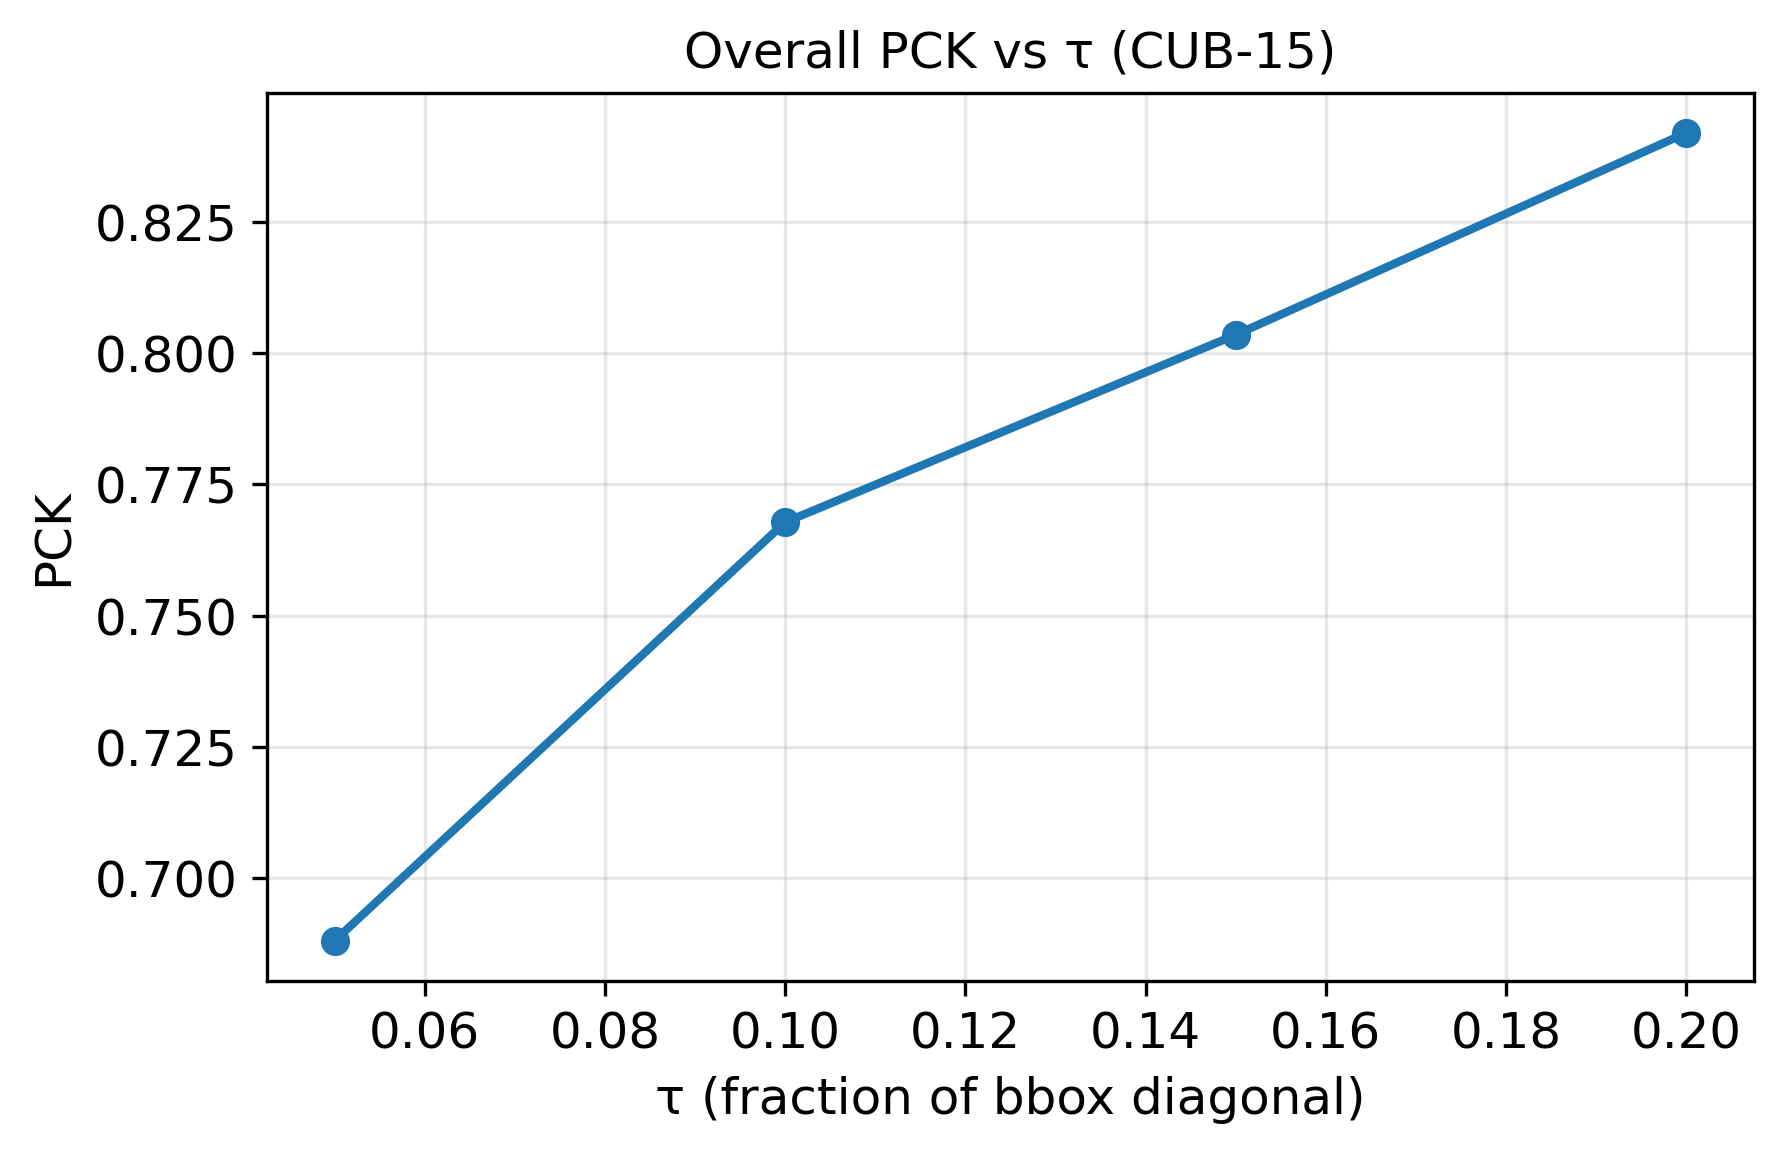
\includegraphics[width=\linewidth,height=\TopCellH]{figures/ReportFigures/pck_overall_curve.png}
  \end{minipage}\hspace{1cm}
  \begin{minipage}[t]{0.42\textwidth}
    \raggedright
    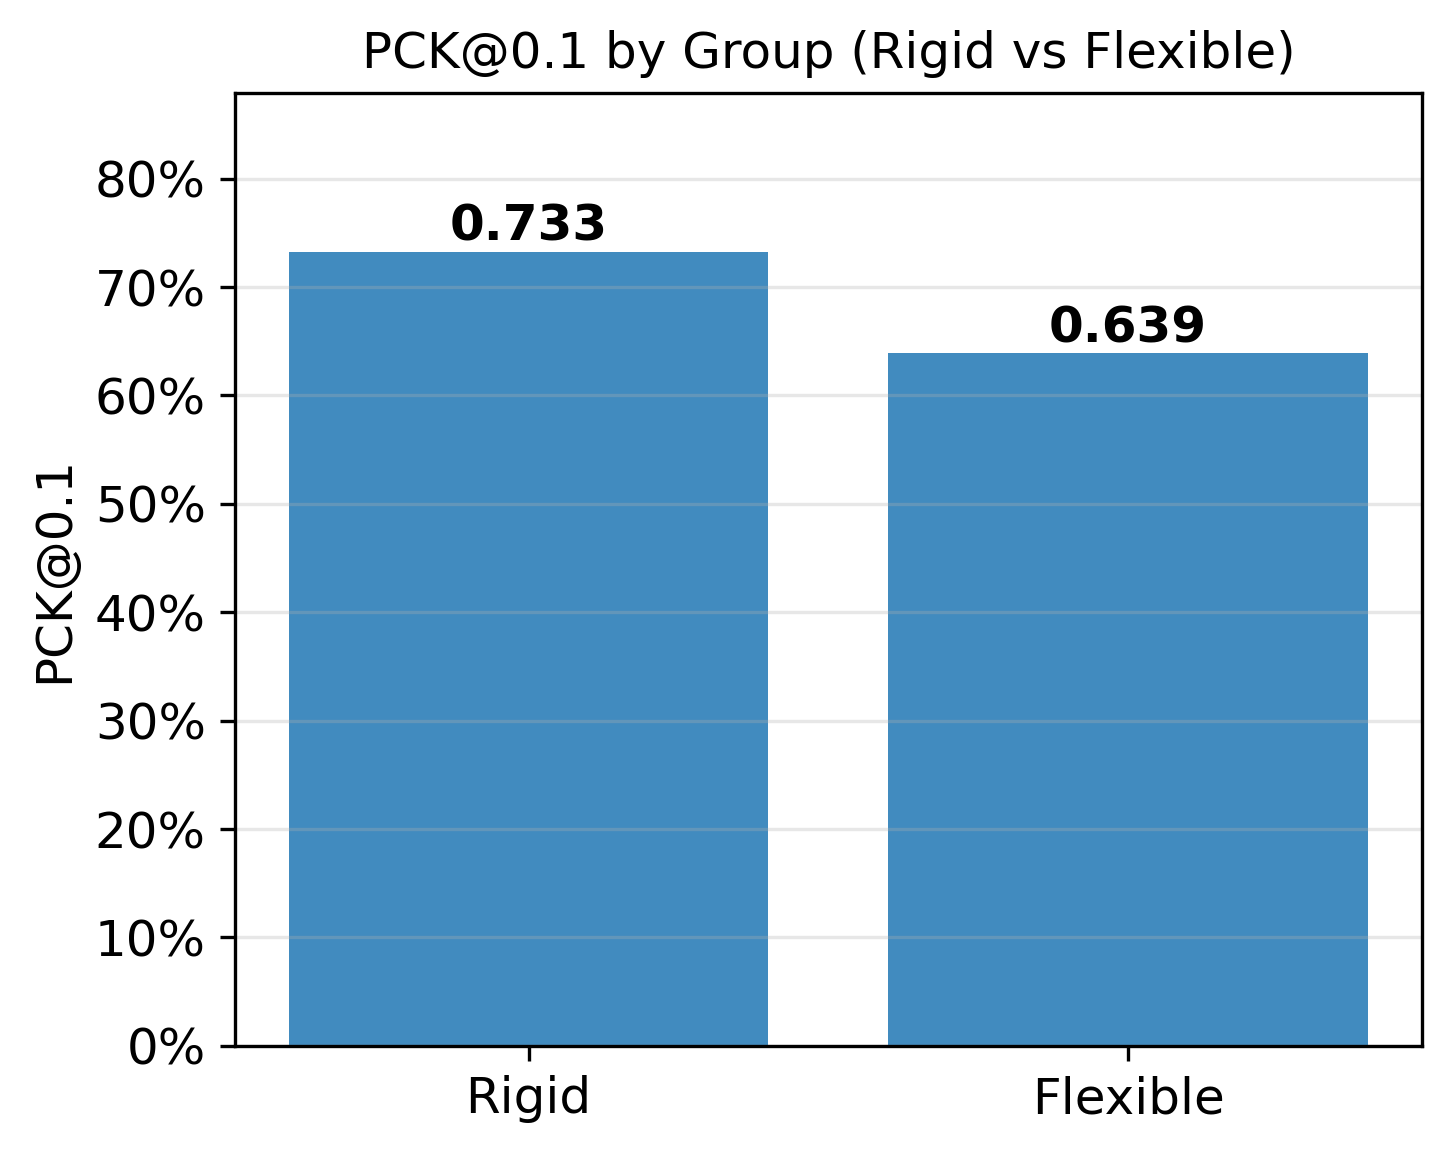
\includegraphics[width=\linewidth,height=4.4cm]{figures/ReportFigures/pck01_rigid_vs_flexible.png}
  \end{minipage}

  % ===== 第二行 =====
  \begin{minipage}[t]{0.49\textwidth}
    \centering
    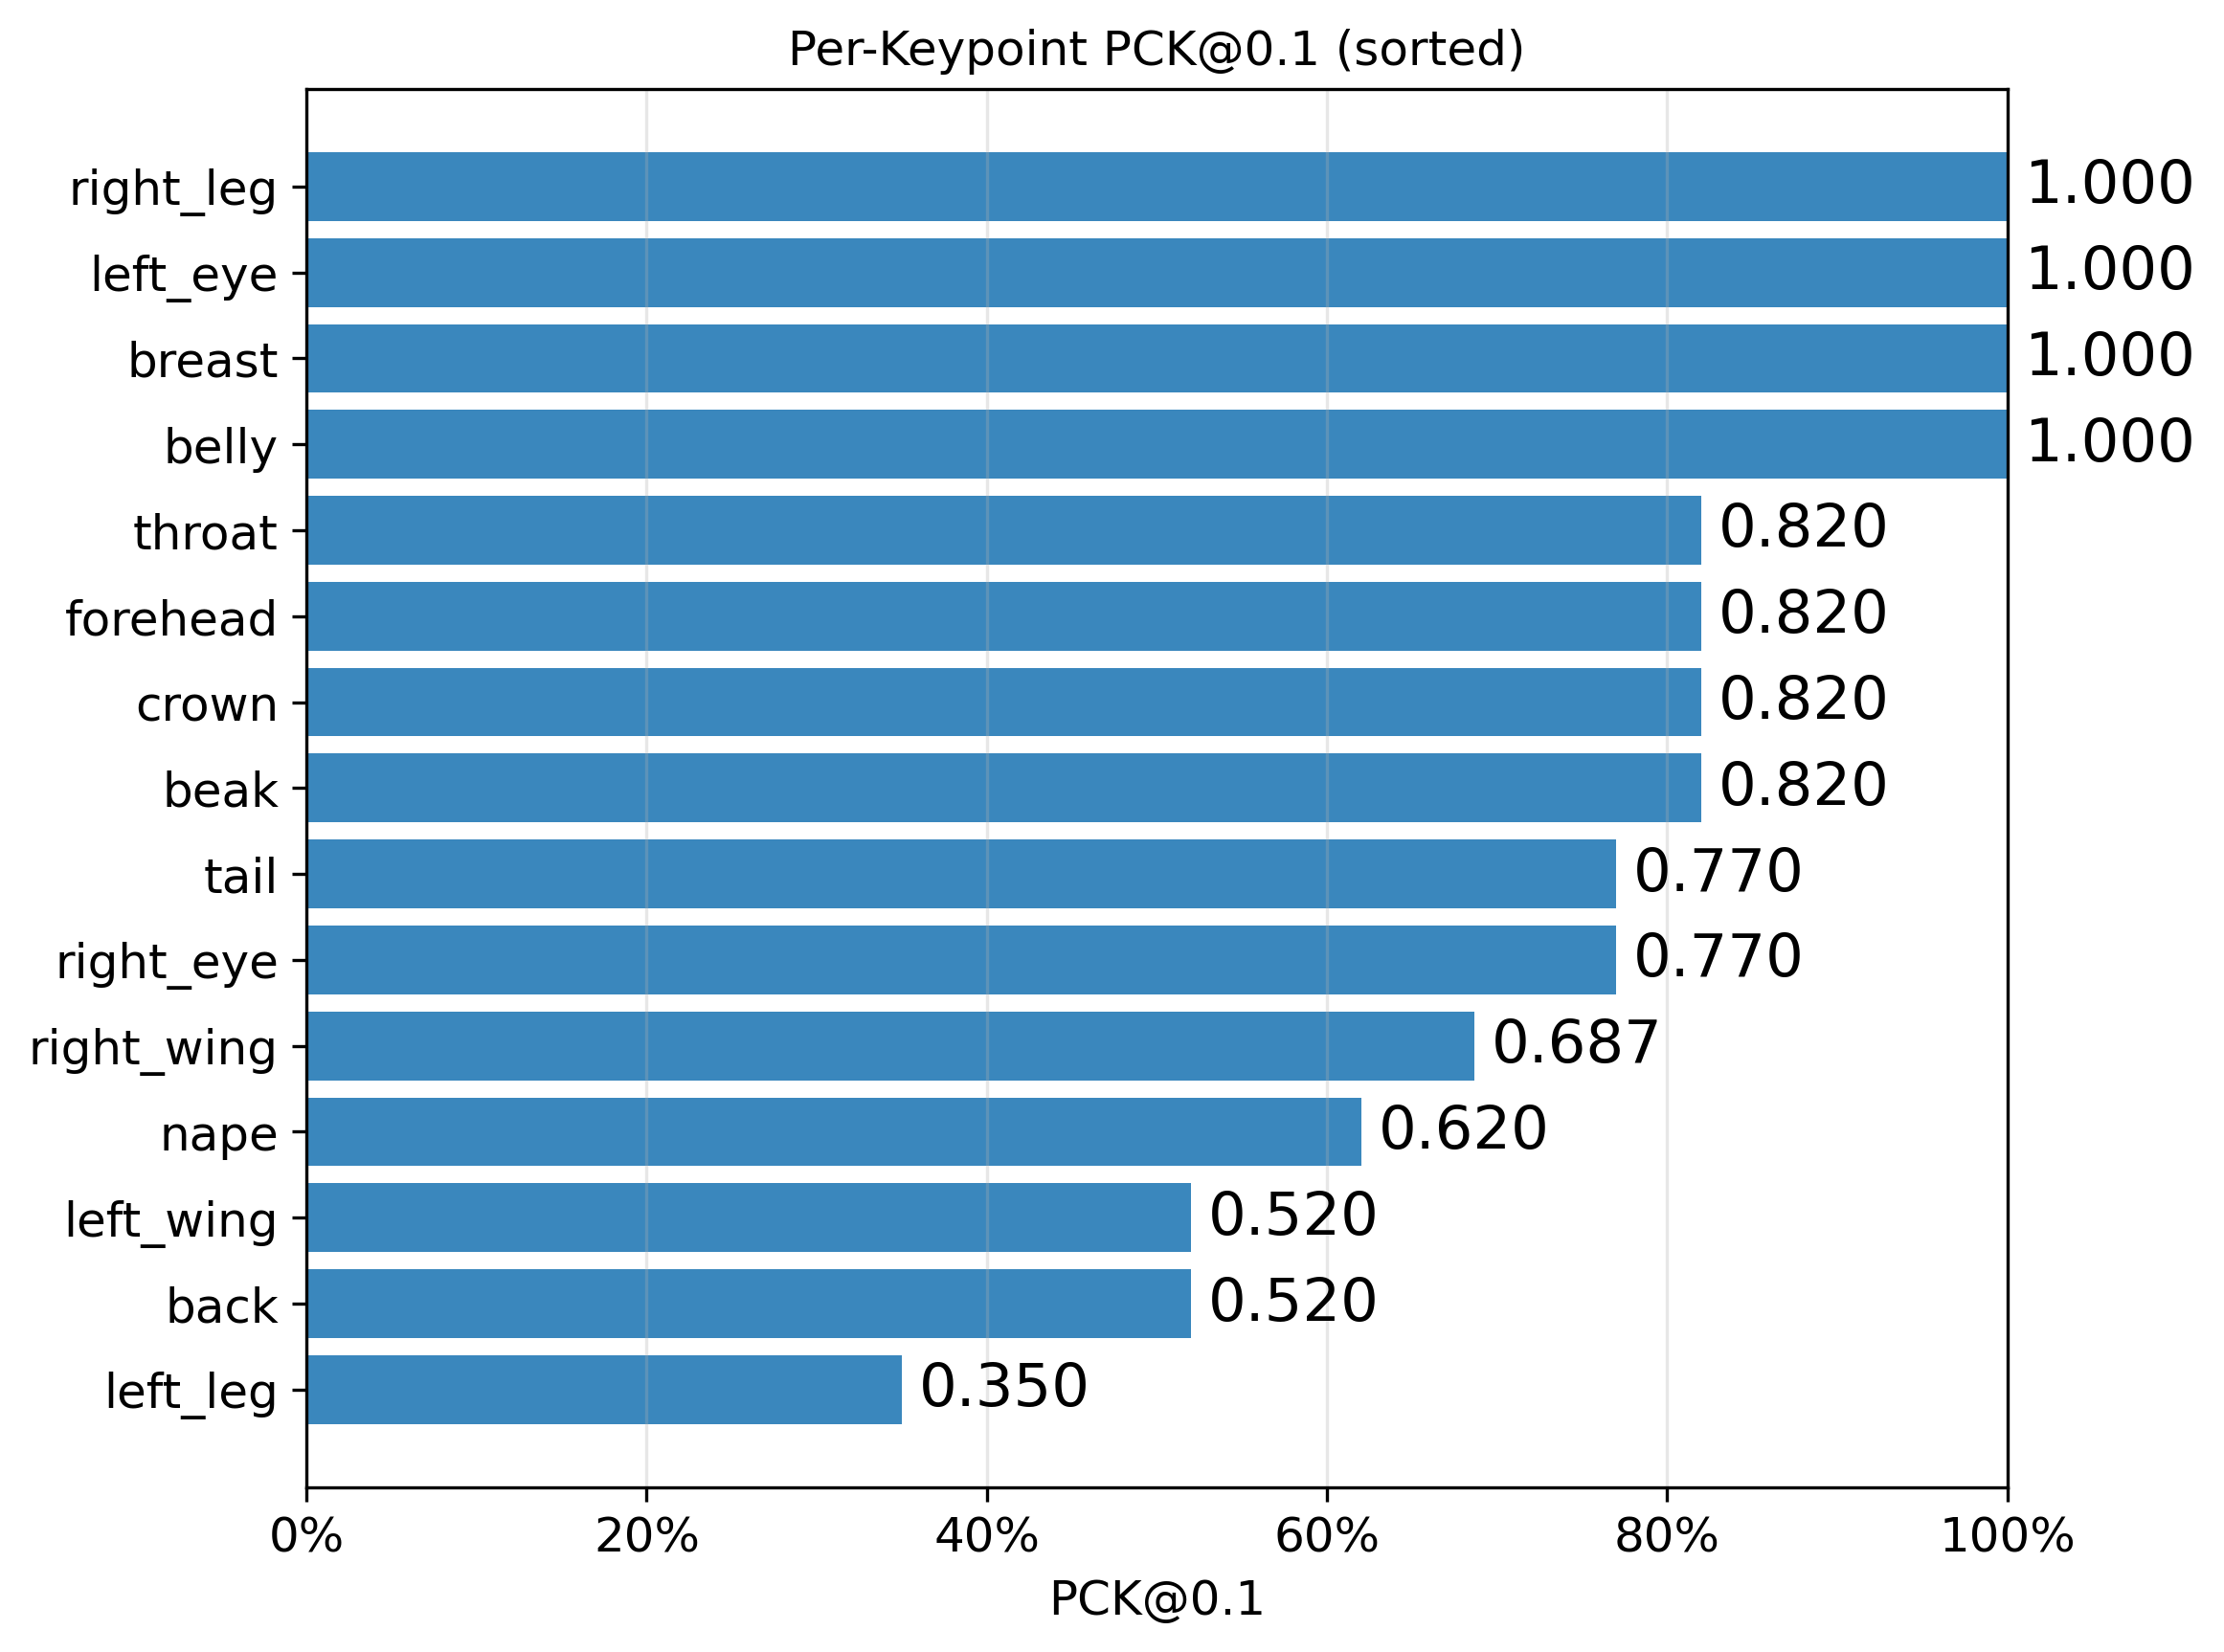
\includegraphics[width=\linewidth,height=\TopCellH]{figures/ReportFigures/pck01_per_keypoint_sorted.png}
  \end{minipage}\hfill
  \begin{minipage}[t]{0.49\textwidth}
    \centering
    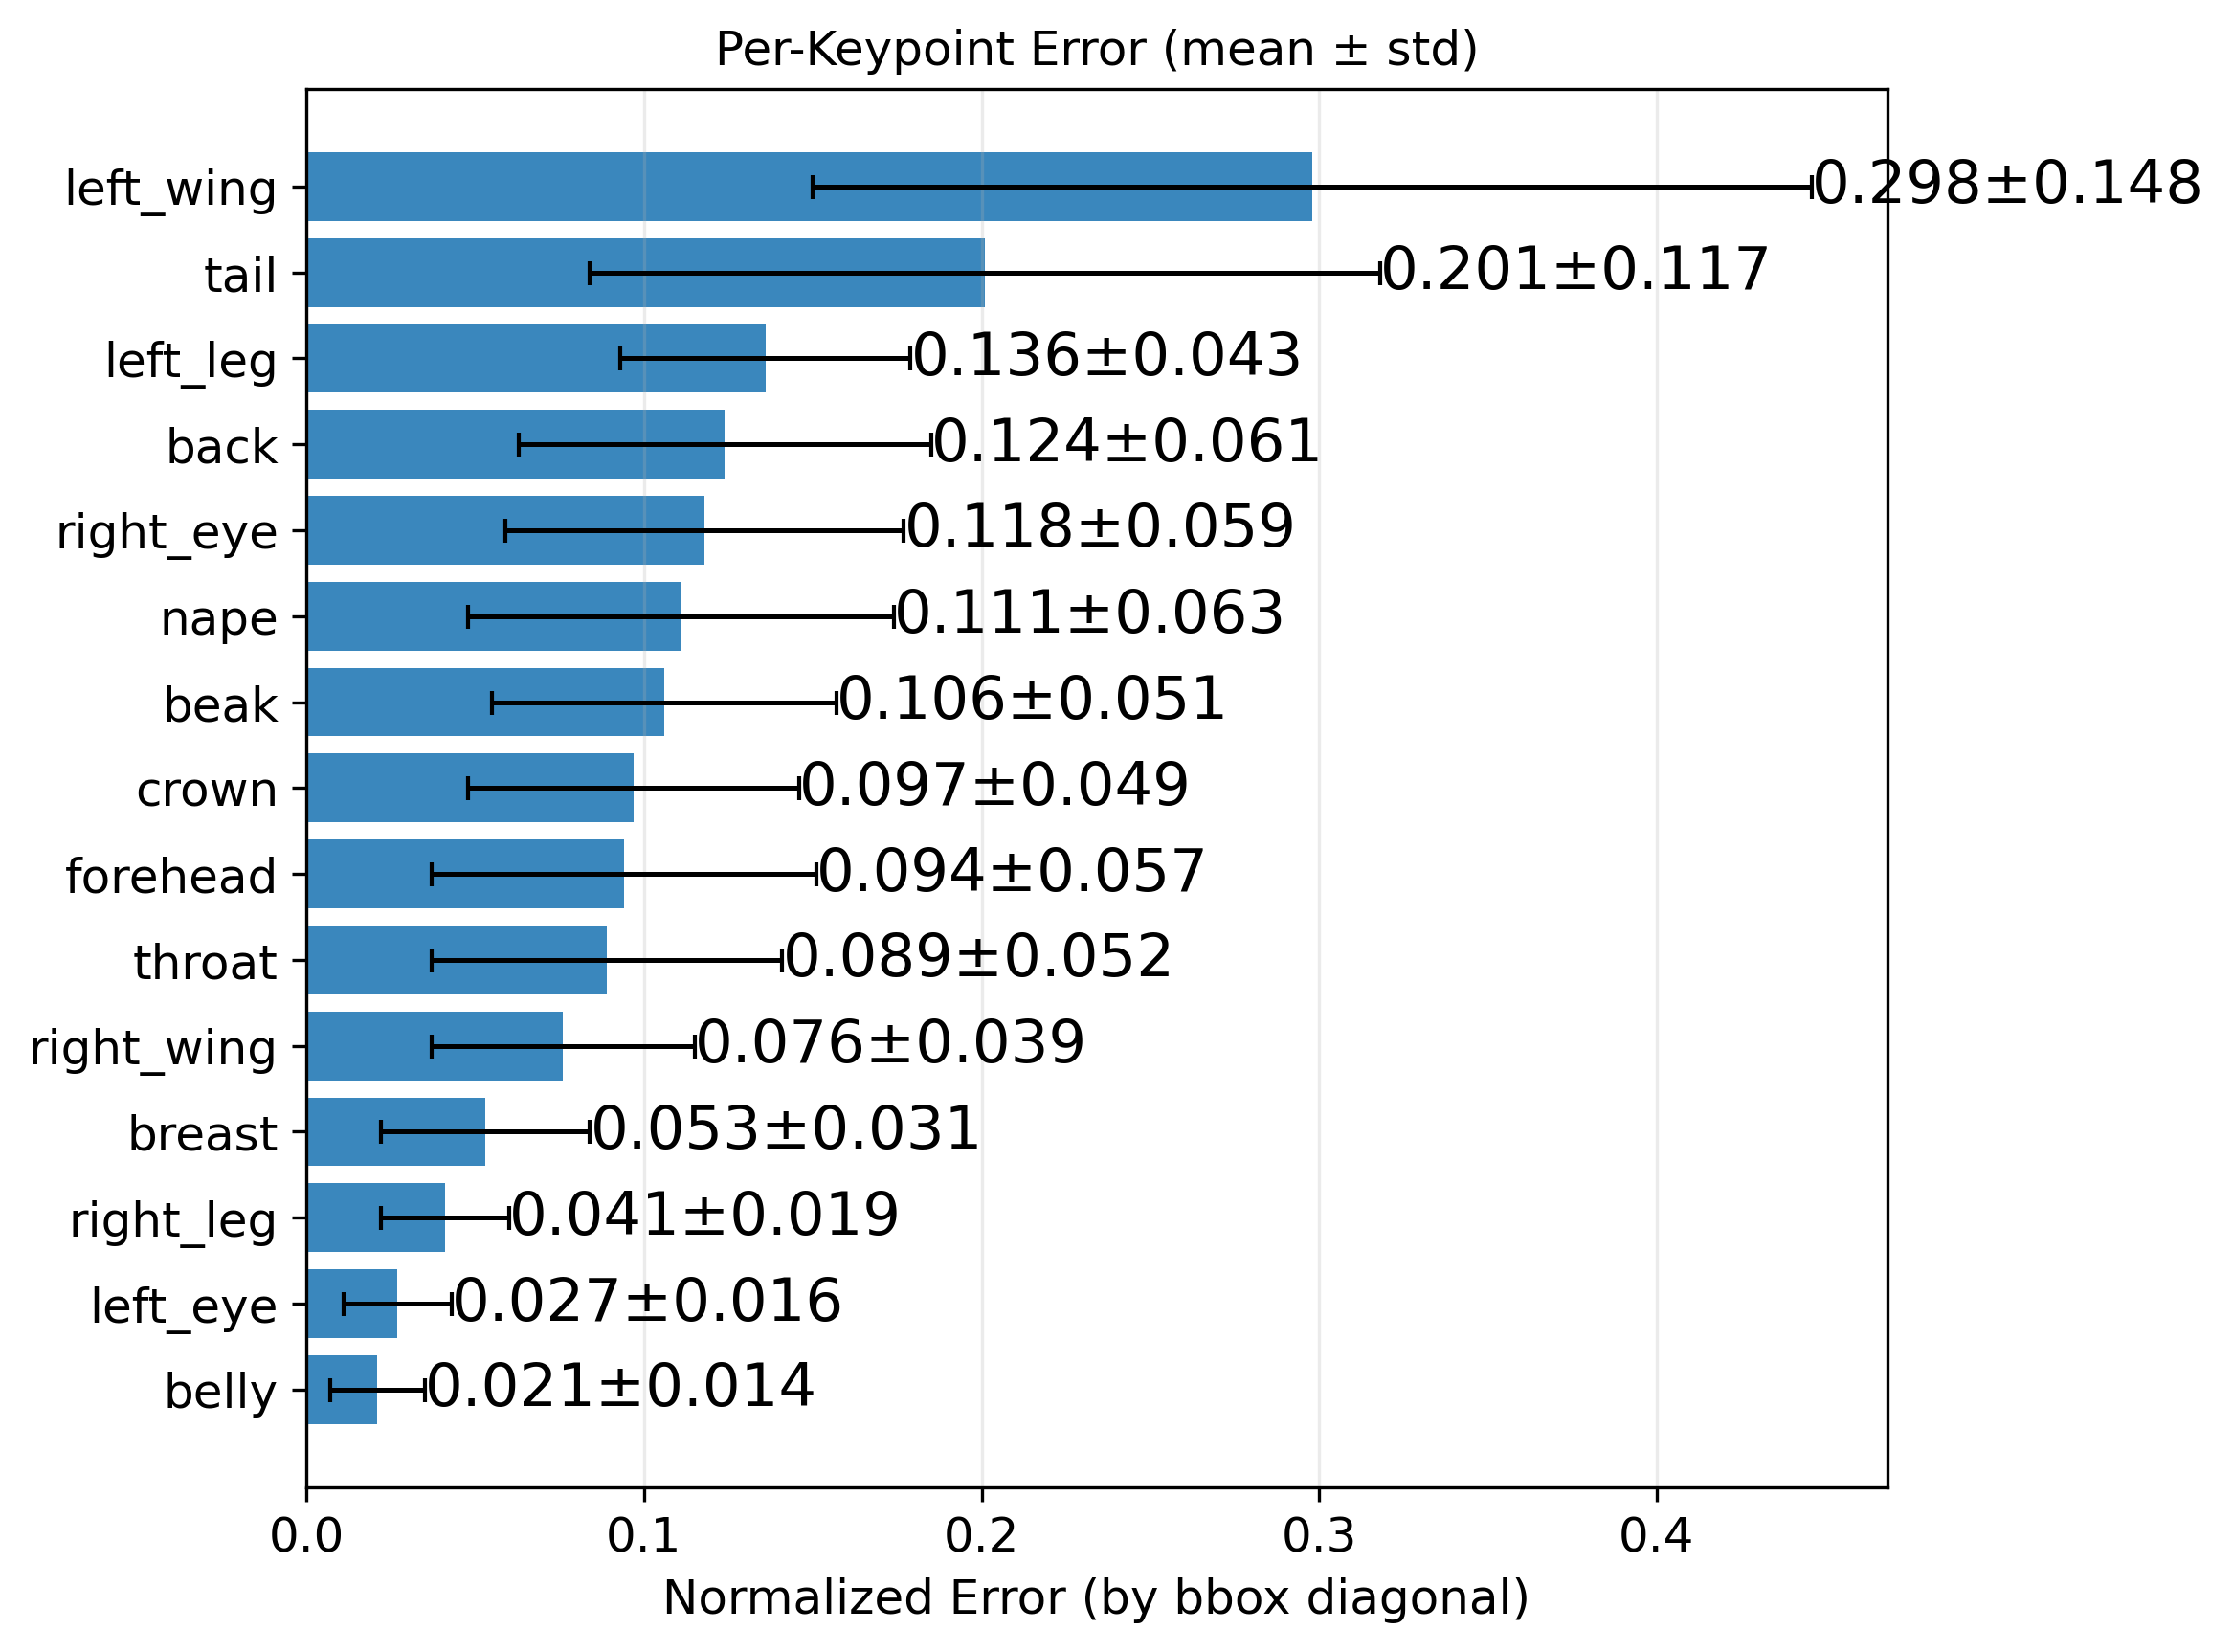
\includegraphics[width=\linewidth,height=\TopCellH]{figures/ReportFigures/error_mean_std.png}
  \end{minipage}

  \caption{HRNet evaluation metrics: (top left) overall PCK curve, (top right) grouped PCK@0.1 (rigid vs flexible), 
(bottom left) per-keypoint PCK@0.1 ranking, and (bottom right) mean and standard deviation of keypoint errors.
}
  \label{fig:hrnet_metrics}
\end{subfigure}

\vspace{0.7em}

% ========= Subfigure B: Bottom row (1x4) =========
\begin{subfigure}[t]{\textwidth}
  \centering
  \begin{minipage}[t]{0.32\textwidth}\centering
    \includegraphics[width=\linewidth,height=\BotCellH]{figures/ReportFigures/Fig1-3.png}
  \end{minipage}\hfill
  \begin{minipage}[t]{0.32\textwidth}\centering
    \includegraphics[width=\linewidth,height=\BotCellH]{figures/ReportFigures/Fig1-2.png}
  \end{minipage}\hfill
  \begin{minipage}[t]{0.32\textwidth}\centering
    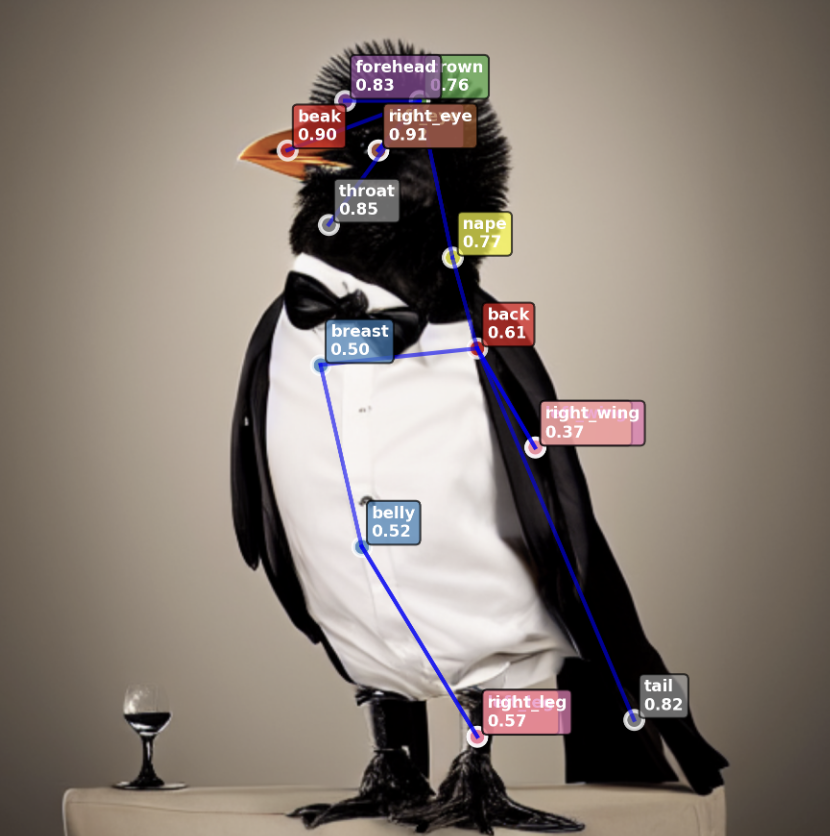
\includegraphics[width=\linewidth,height=\BotCellH]{figures/ReportFigures/Fig1-5.png}
  \end{minipage}
  \caption{Example frames with detected 15-point skeletons from the generated sequence.}
  \label{fig:row_bottom}
\end{subfigure}

\caption{HRNet evaluation and output examples.}
\label{fig:two-rows-one-figure}
\end{figure}






\subsection{Pose Sequence Generation using MDM}
% The Motion Diffusion Model (MDM) demonstrates stable convergence. As shown in Fig.\ref{fig:train_curves}(left), both training and validation MSE decrease steadily over the first 50 epochs, with validation consistently lower since training batches include augmentation and noise, whereas validation is evaluated on clean sequences. Fig.\ref{fig:train_curves}(right) shows the normalised Skeleton and Range losses, which drop rapidly before reaching a stable plateau. Skeleton loss is computed as averaged bone-length error, and Range loss as normalised coordinate deviations, both scaled to a comparable $0$--$1$ range. These results confirm that MDM learns smooth, temporally coherent motion while preserving anatomical plausibility, providing reliable skeleton trajectories for downstream video synthesis.

% Fig \ref{fig:bottom_five} shows five samples from a 64-frame sequence illustrate a plausible landing motion. Colors indicate head (red), torso and tail (blue), wings (orange), and legs (green). The torso pitches up while descending, wings flare symmetrically into a braking posture, the tail stabilizes attitude, and the legs extend in preparation for contact. The sequence shows anatomically consistent kinematics: the body center descends smoothly, wings transition from downstroke to flare with bilateral symmetry, the tail remains aligned with the torso, and the legs progressively extend forward. Overall, the poses remain well-formed, with no bone crossings or jitter, indicating that the model has learned a coherent landing pattern.

The Motion Diffusion Model (MDM) was trained on 64-frame sequences with six action labels. 
As shown in Fig.~\ref{fig:train_curves}(left), both training and validation MSE decreased steadily over the first 50 epochs. 
Fig.~\ref{fig:train_curves}(right) shows the normalised Skeleton and Range losses, which dropped rapidly before stabilising at low values. 
Skeleton loss was computed as the averaged bone-length error, and Range loss as normalised coordinate deviations, both scaled to a comparable $0$--$1$ range.  

Representative samples from a generated 64-frame landing sequence are shown in Fig.~\ref{fig:bottom_five}. 
The torso pitched upwards while descending, wings flared symmetrically into a braking posture, the tail aligned with the torso to stabilise attitude, and the legs extended forward in preparation for contact. 
The sequence remained free of bone crossings or frame-level jitter, and individual poses appeared anatomically consistent across time.



\begin{figure}[H]
\centering

% ===== Subfigure (a): TOP, two plots centered & larger =====
  \begin{subfigure}[t]{0.95\textwidth}
    \centering
    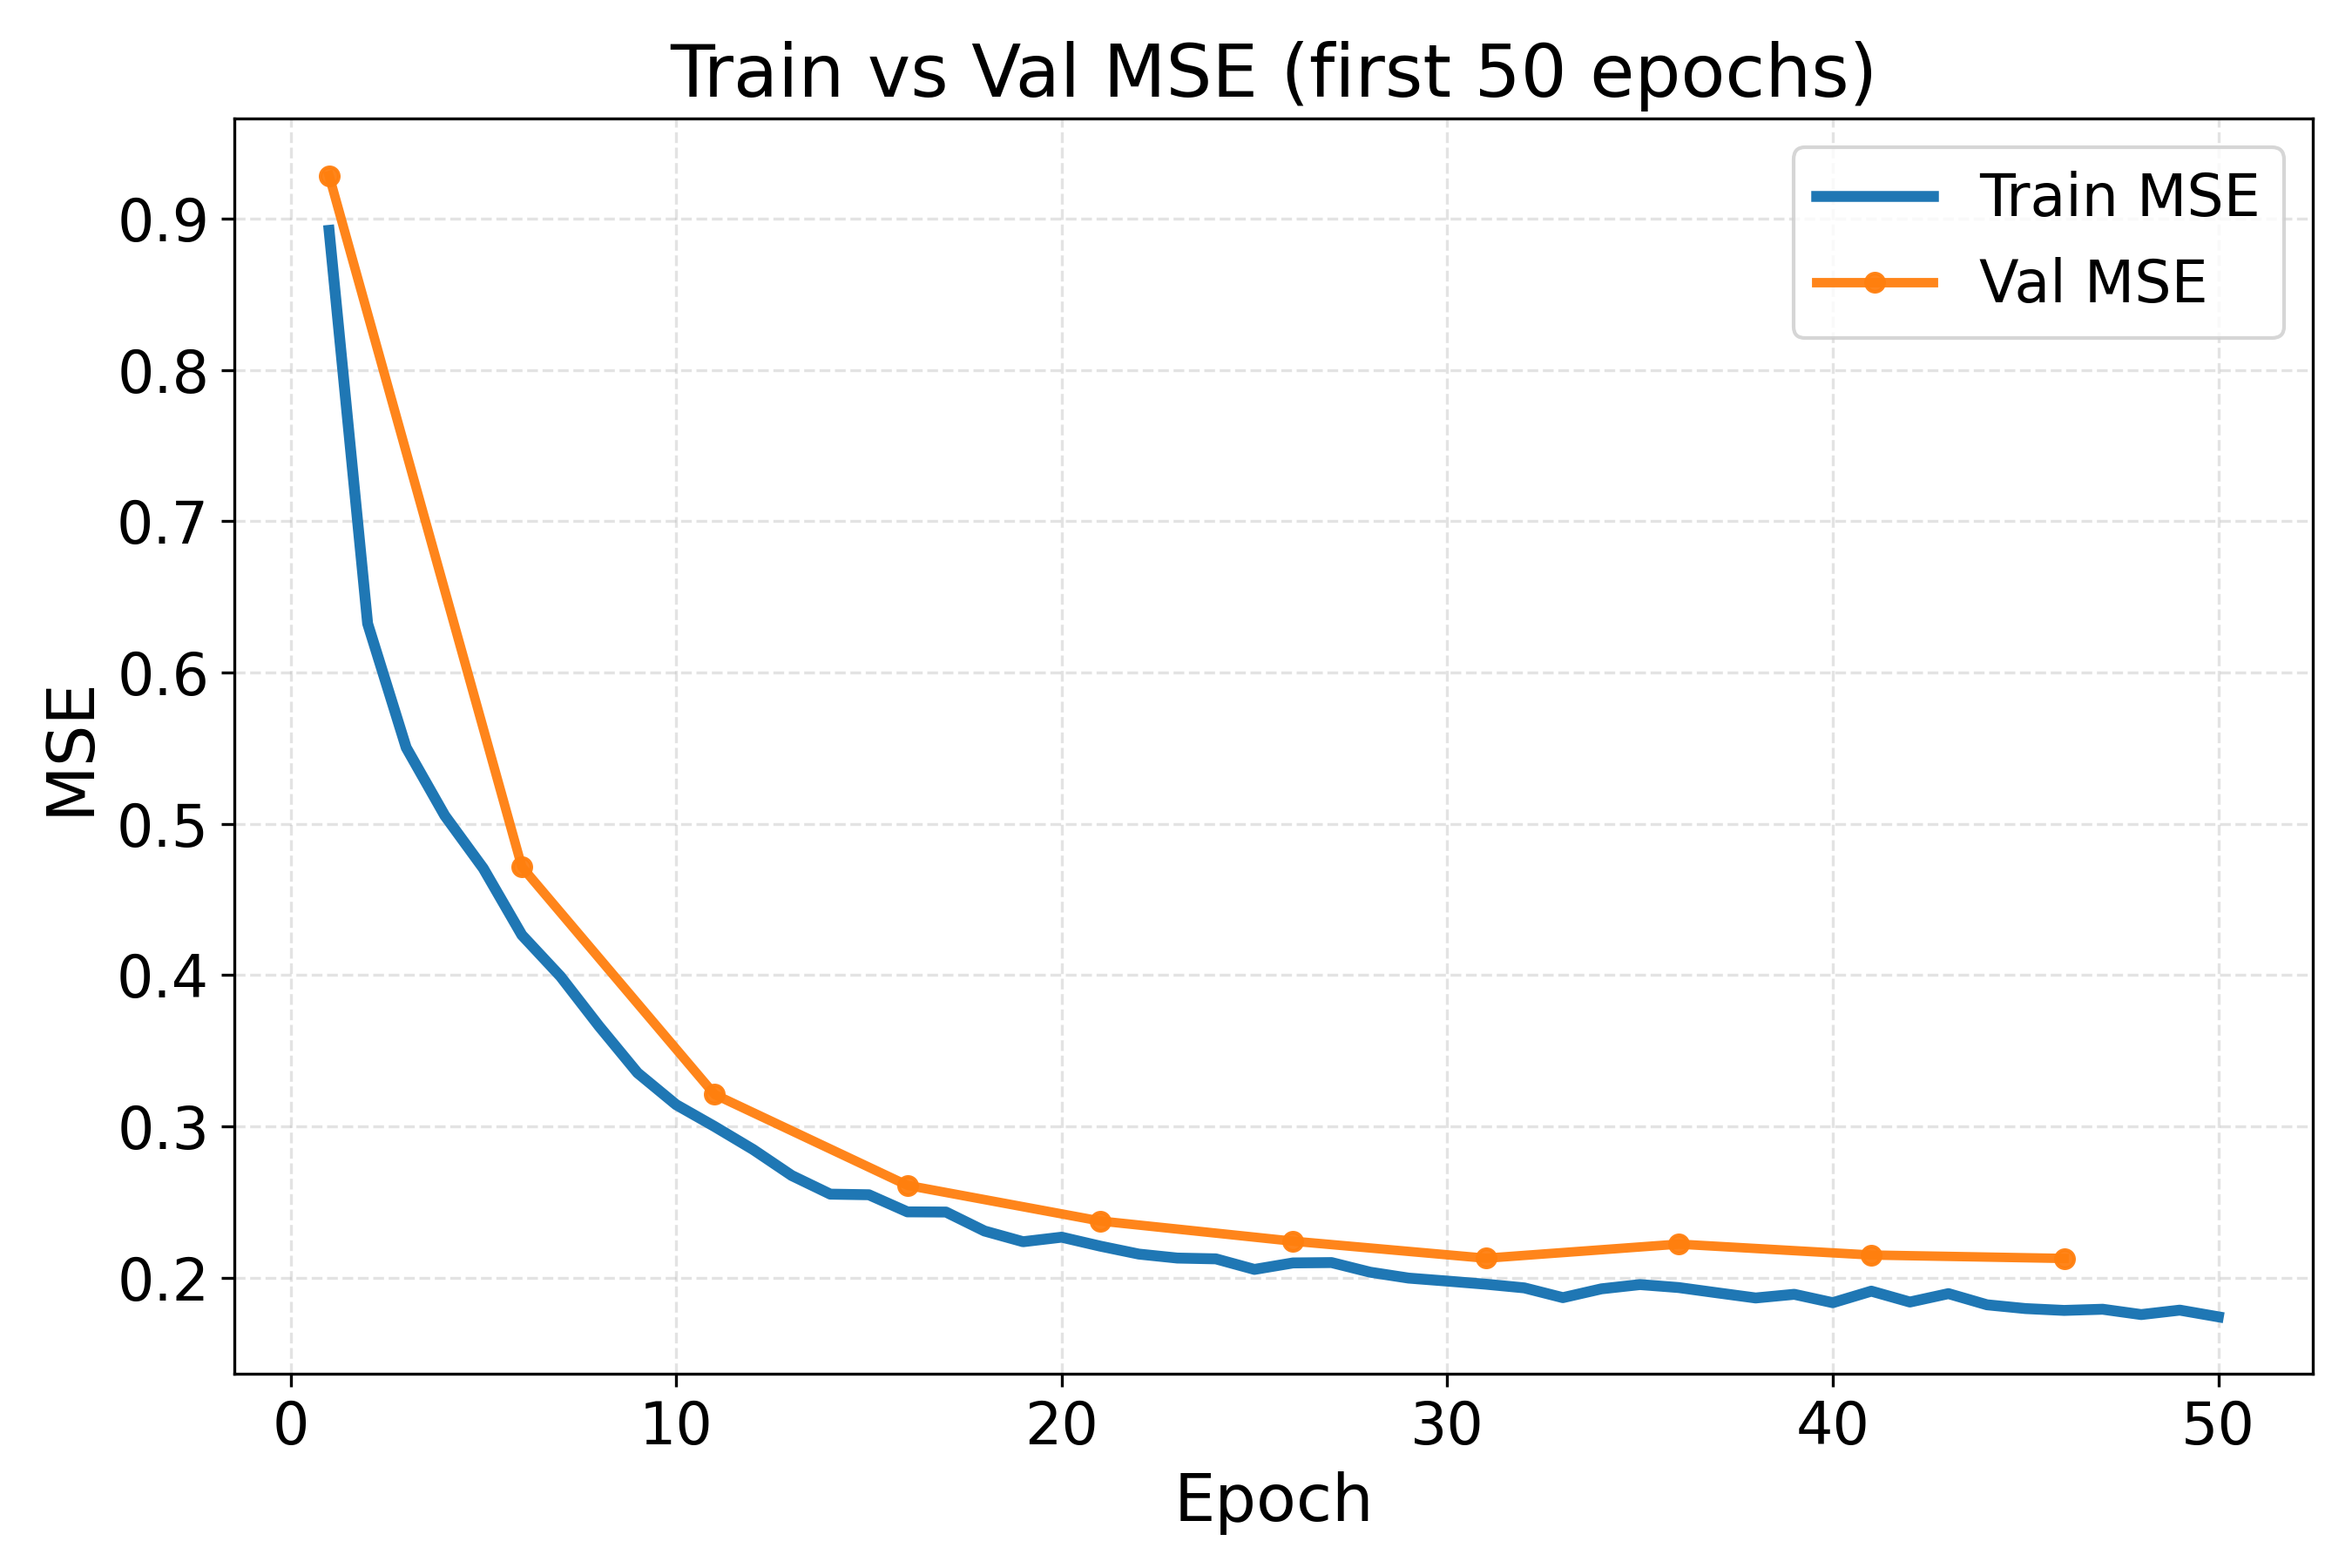
\includegraphics[width=0.48\linewidth]{figures/ReportFigures/A1.png}
    \hfill
    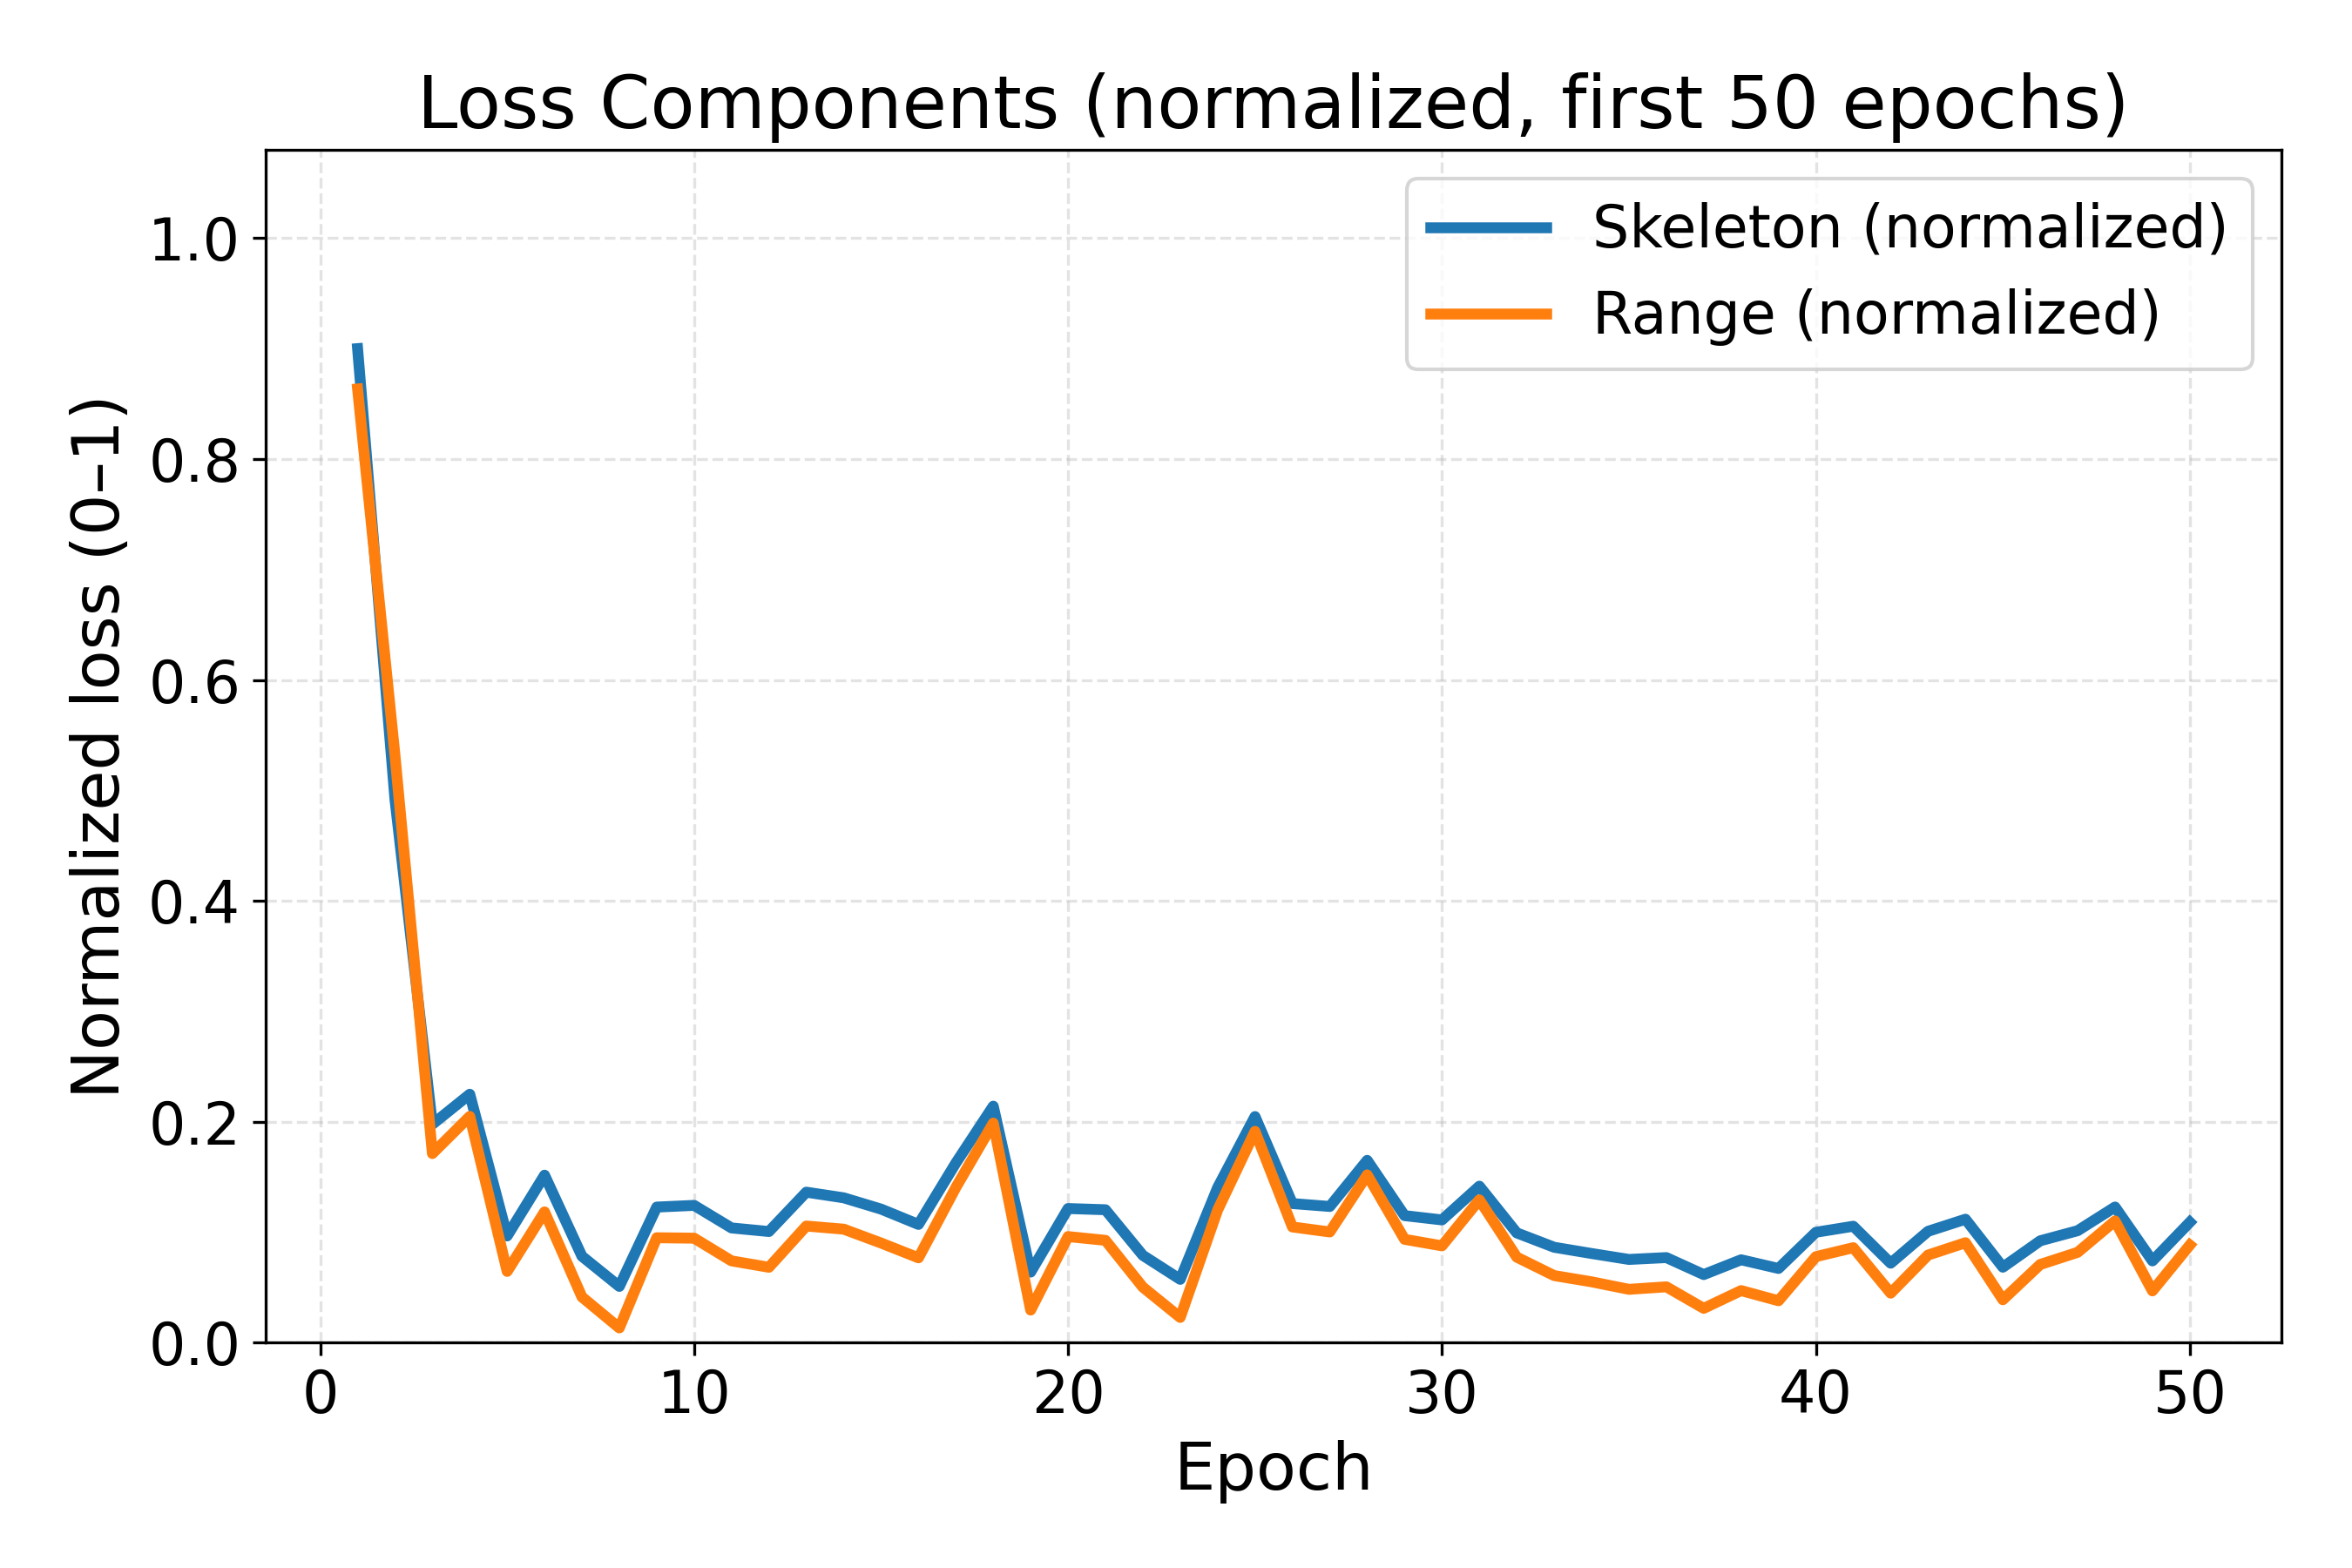
\includegraphics[width=0.48\linewidth]{figures/ReportFigures/A2.png}
    \caption{Training curves (first 50 epochs): 
    (left) Train vs Val MSE; (right) Skeleton and Range losses.}
    \label{fig:train_curves}
  \end{subfigure}

\vspace{0.9em}

% ===== Subfigure (b): BOTTOM, 1x5 frames =====
\begin{subfigure}[t]{\textwidth}
  \centering
  \begin{minipage}{0.8\textwidth}
    \centering
    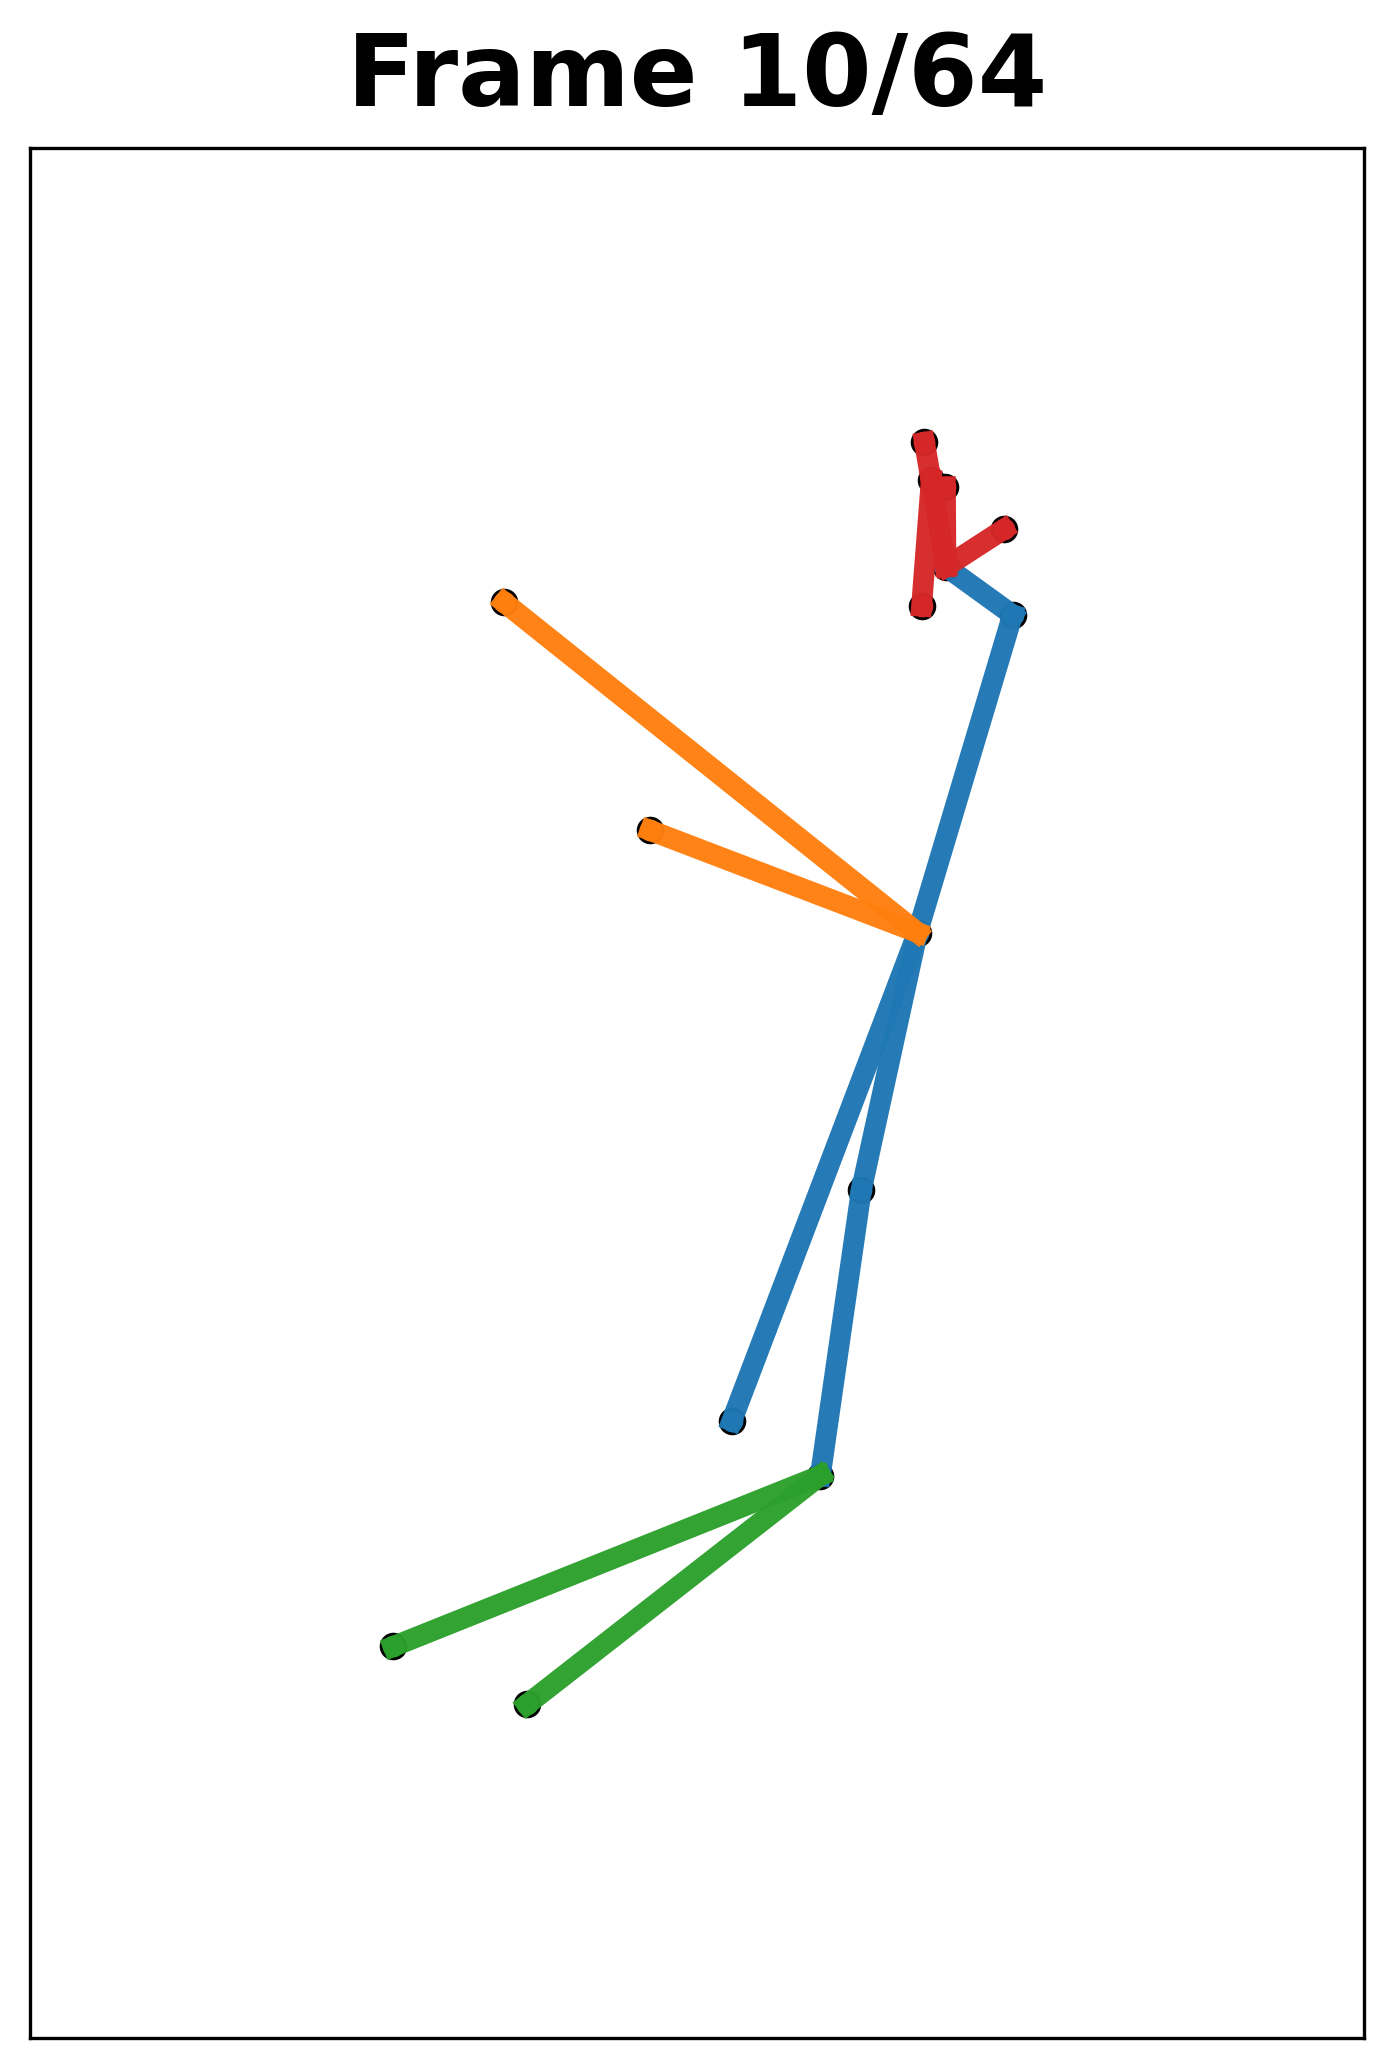
\includegraphics[width=0.16\textwidth,scale=0.8,height=3cm]{figures/ReportFigures/frame_010.png}\hfill
    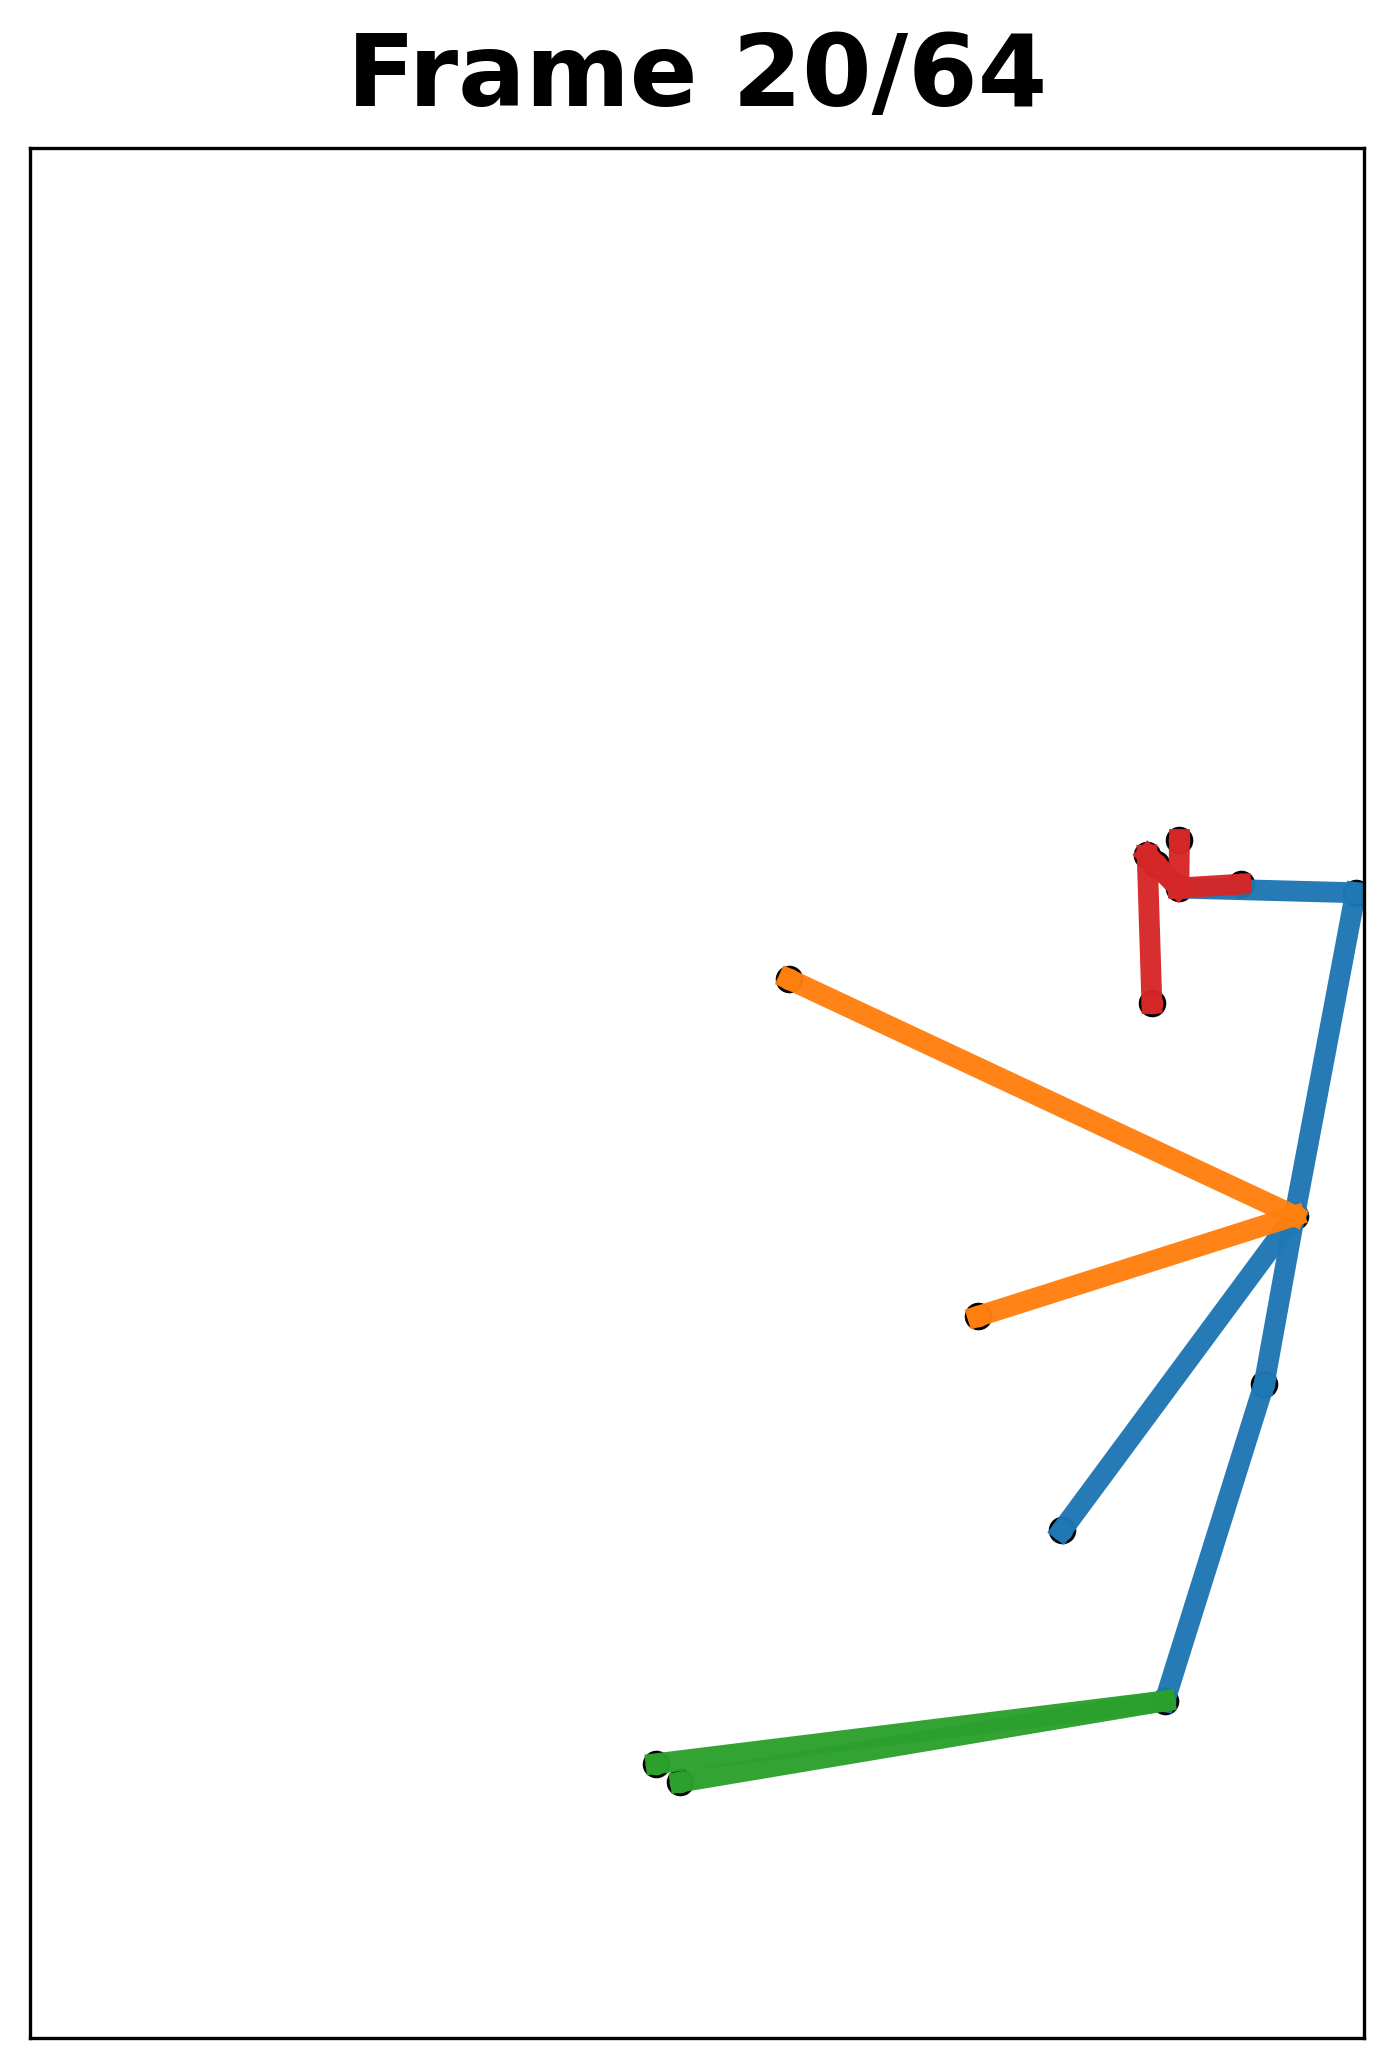
\includegraphics[width=0.16\textwidth,scale=0.8,height=3cm]{figures/ReportFigures/frame_020.png}\hfill
    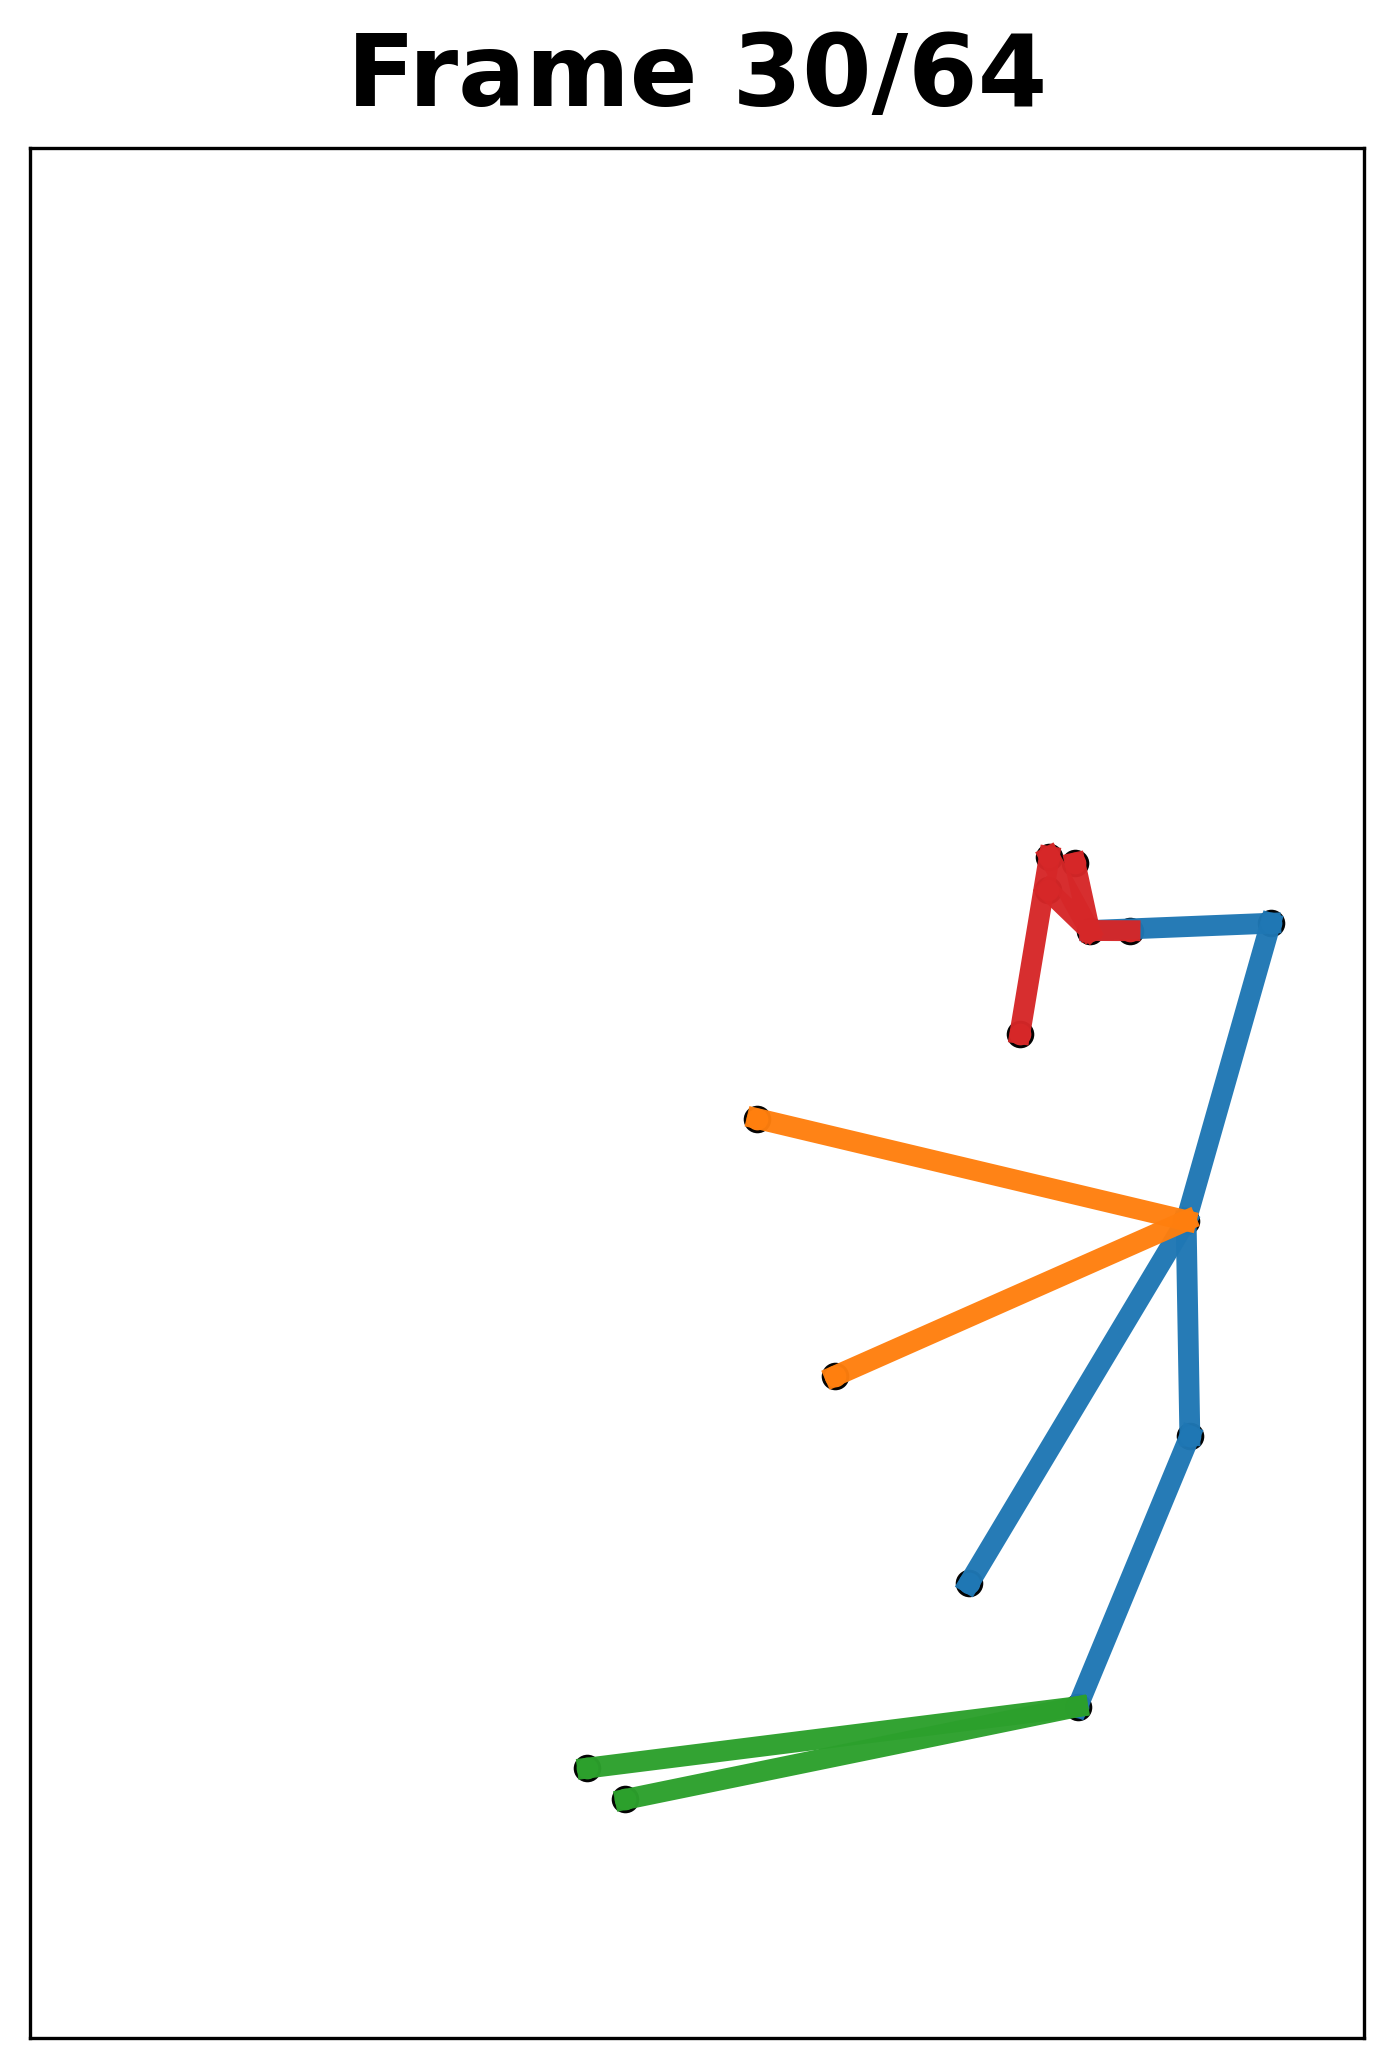
\includegraphics[width=0.16\textwidth,scale=0.8,height=3cm]{figures/ReportFigures/frame_030.png}\hfill
    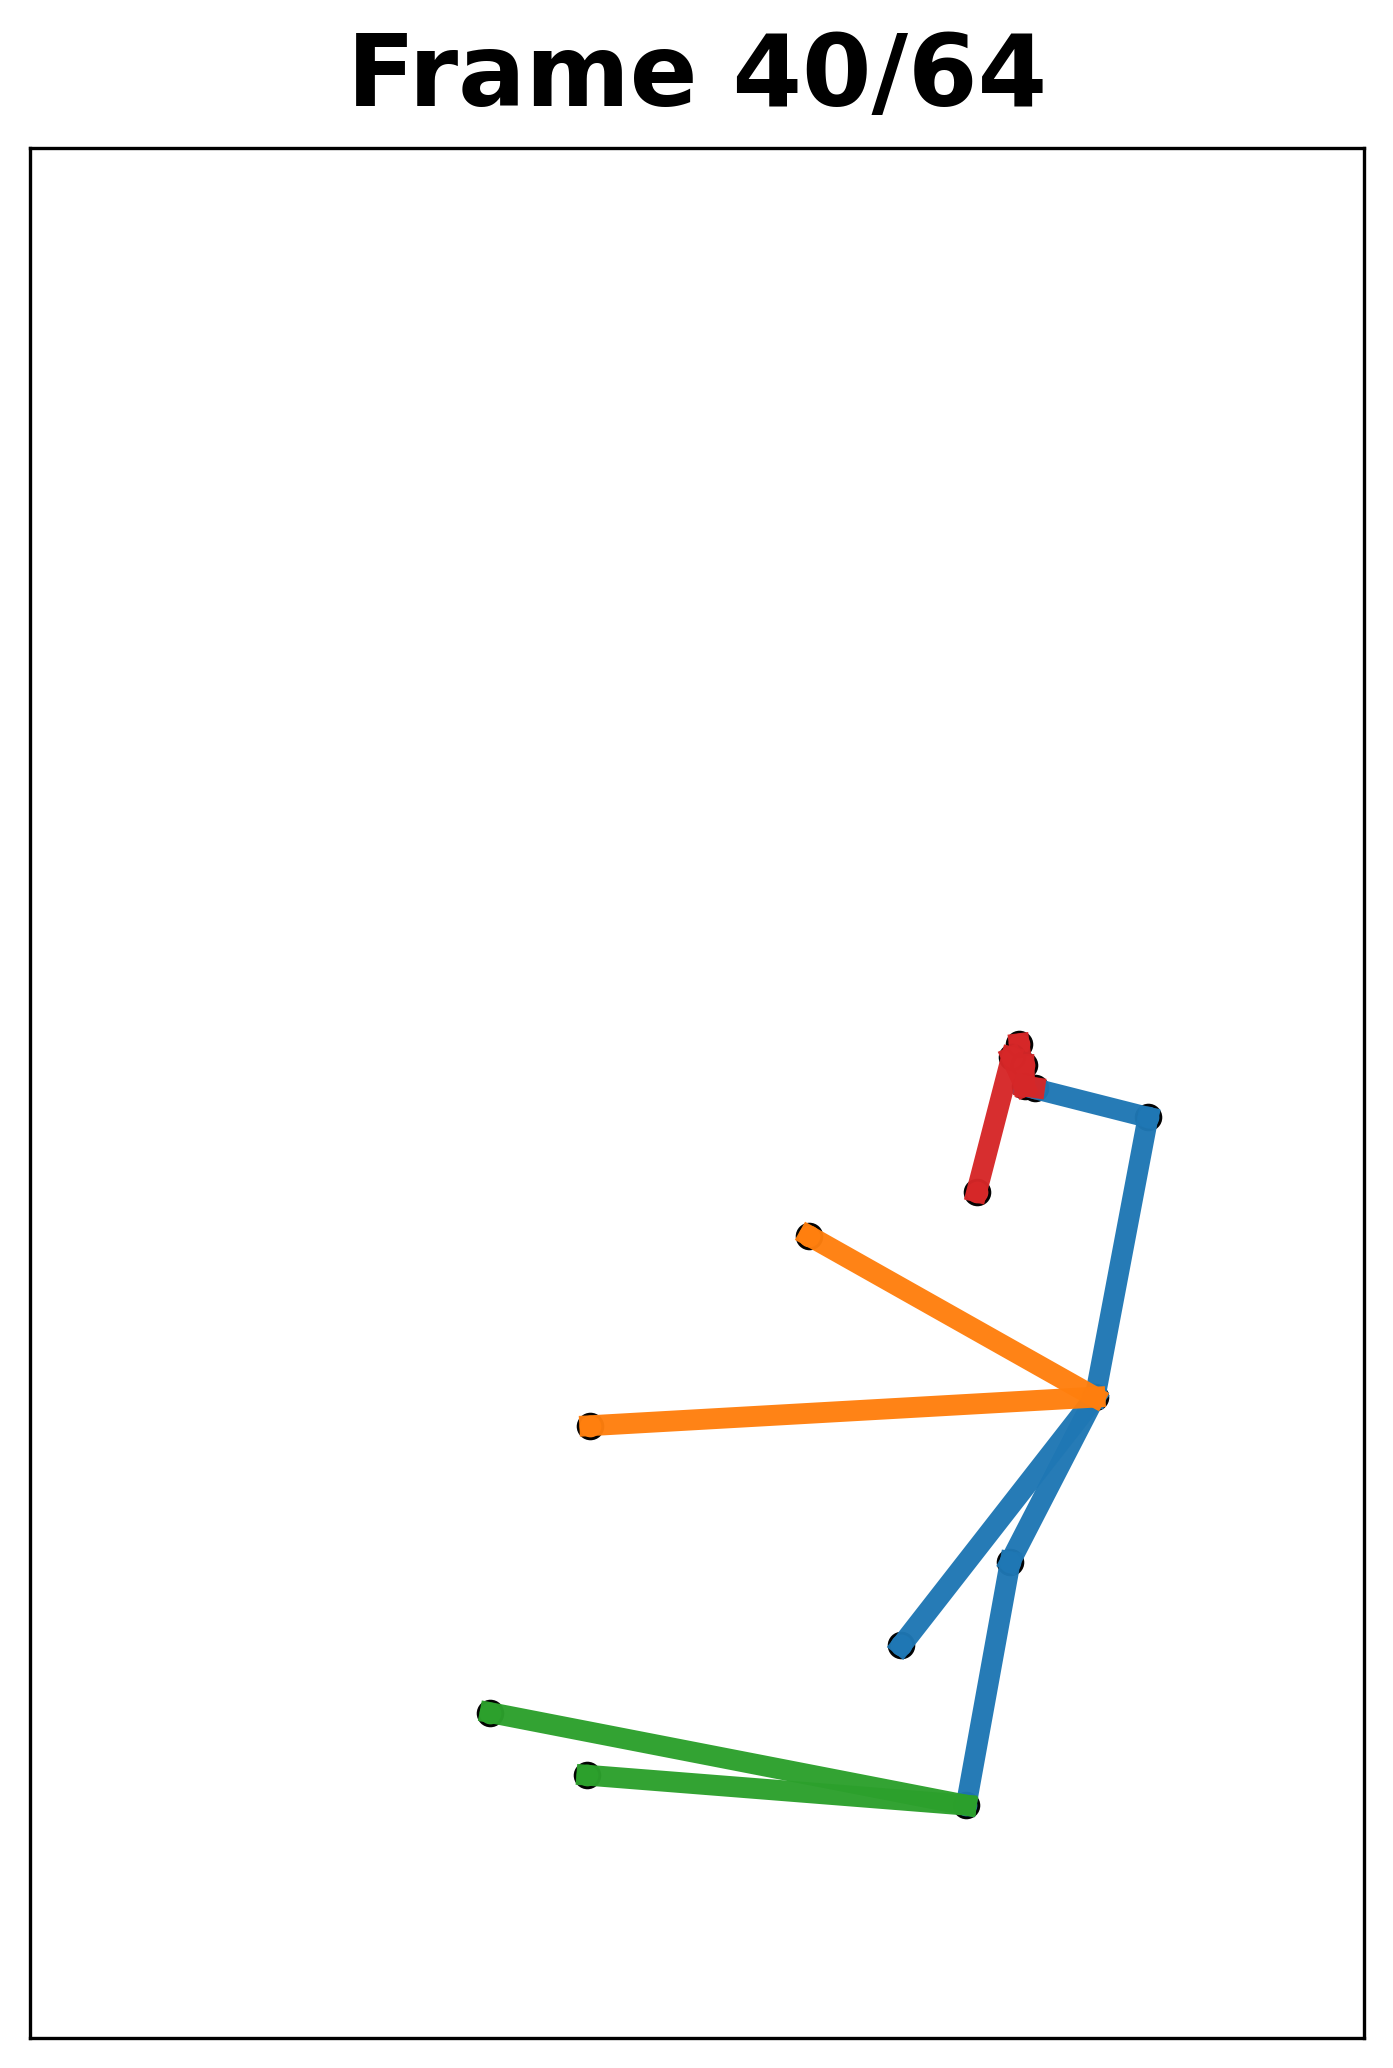
\includegraphics[width=0.16\textwidth,scale=0.8,height=3cm]{figures/ReportFigures/frame_040.png}\hfill
    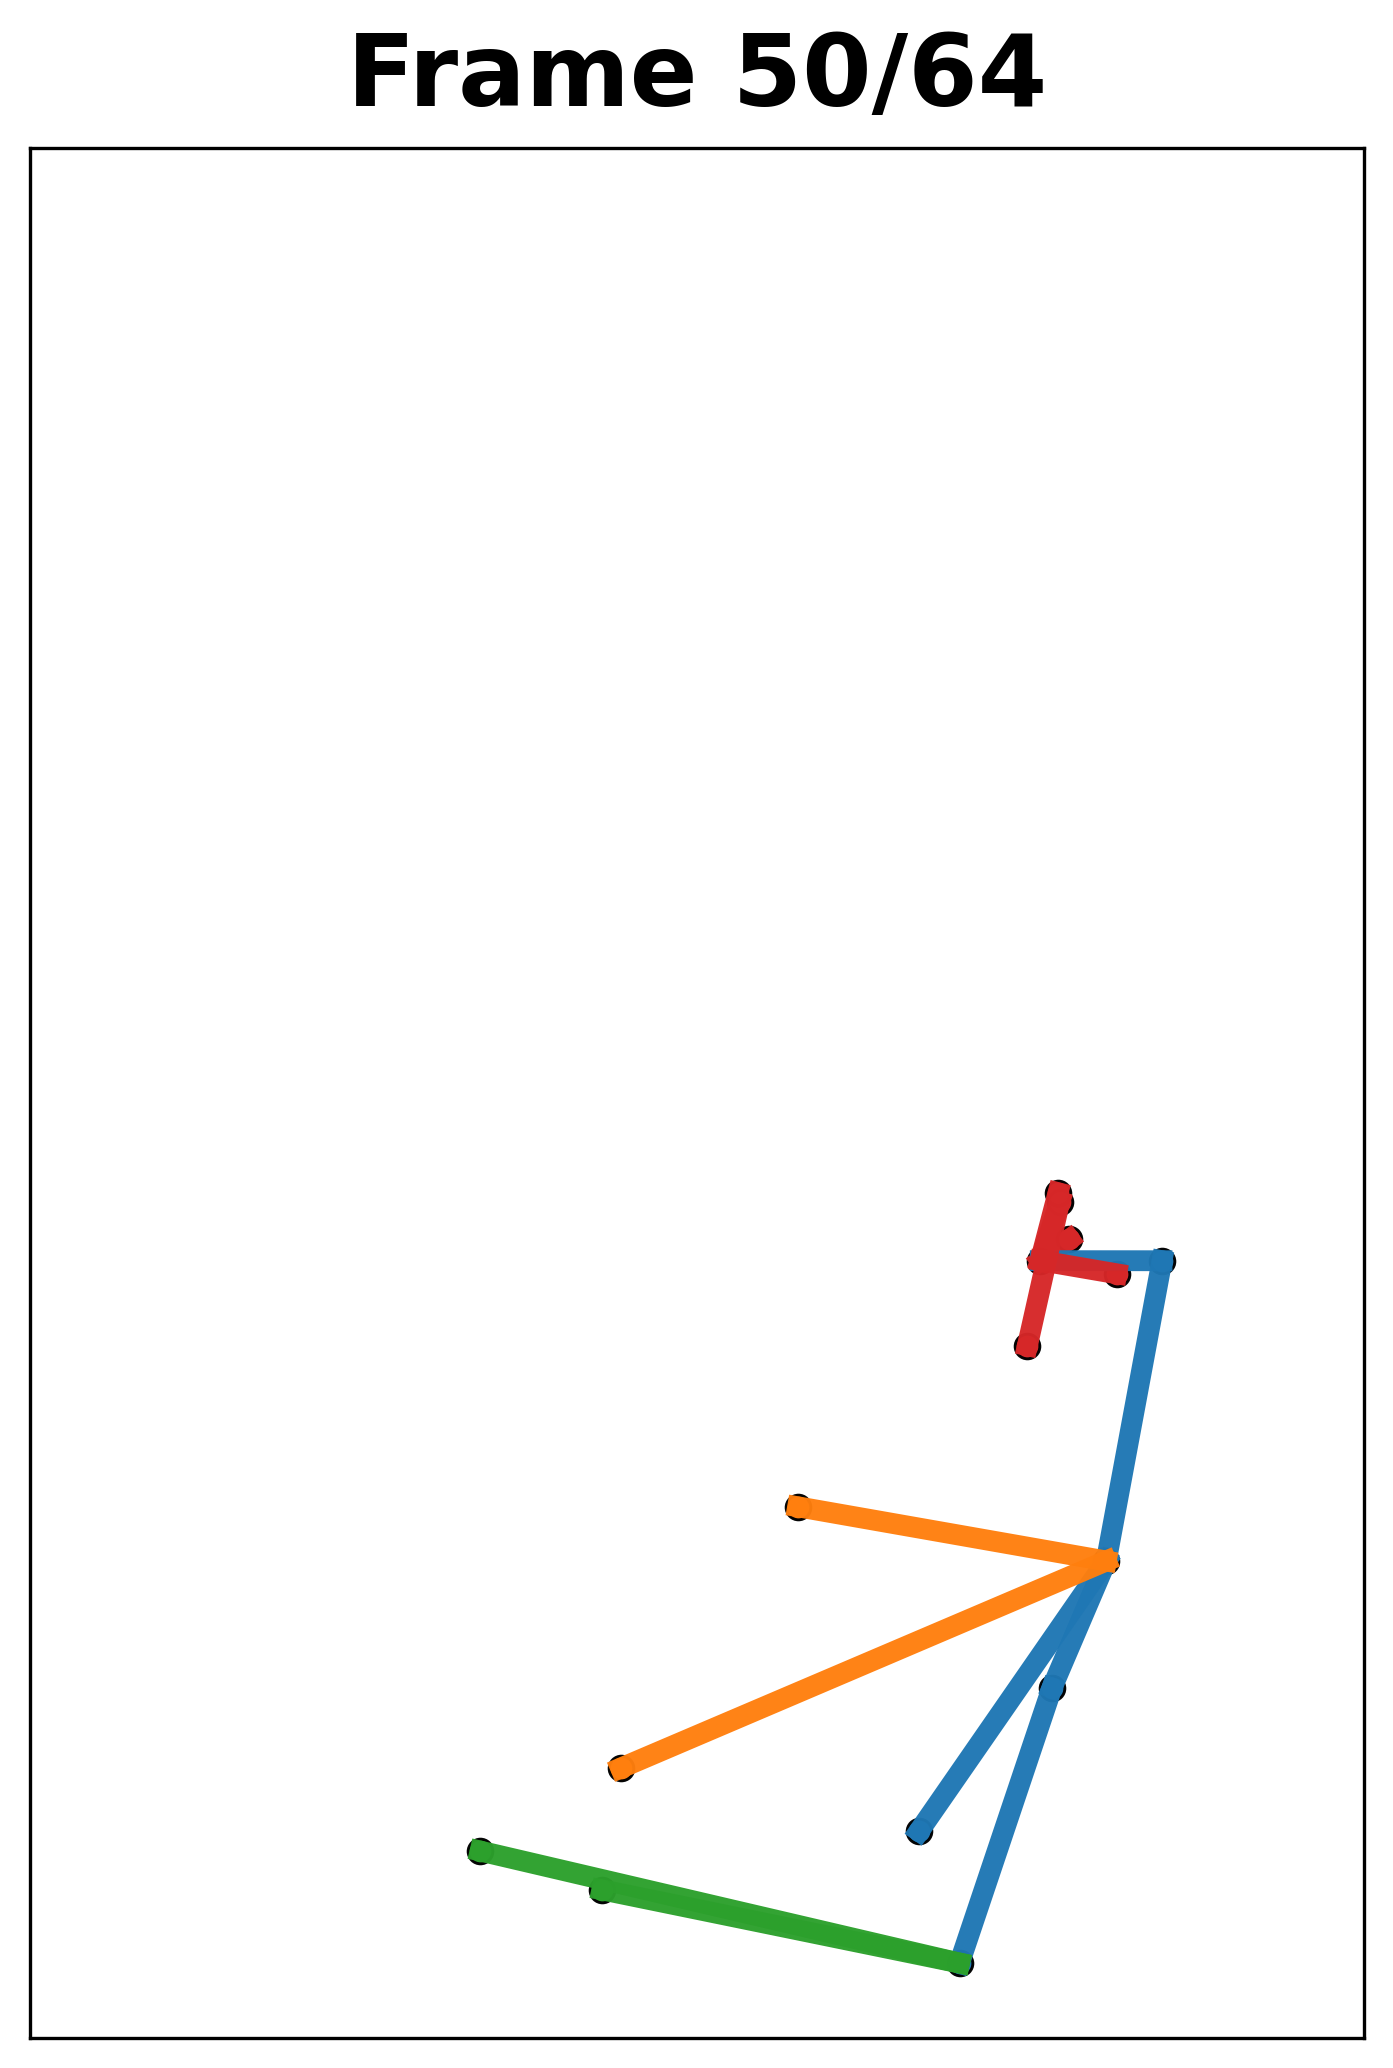
\includegraphics[width=0.16\textwidth,scale=0.8,height=3cm]{figures/ReportFigures/frame_050.png}
  \end{minipage}

  \caption{Sample frames from the generated sequence.}
  \label{fig:bottom_five}
\end{subfigure}


\caption{Overall caption combining training curves and sample frames.}
\label{fig:combined_onefigure}
\end{figure}


% \begin{figure}[H]
% \centering
% \begin{subfigure}[t]{0.3\textwidth}
%   \centering
%   \includegraphics[width=\linewidth]{figures/ReportFigures/A1_train_val_mse_0_50.png}
%   \caption{Left panel caption}
%   \label{fig:left}
% \end{subfigure}\hfill
% \begin{subfigure}[t]{0.3\textwidth}
%   \centering
%   \includegraphics[width=\linewidth]{figures/ReportFigures/A2_train_loss_components_0_50.png}
%   \caption{Right panel caption}
%   \label{fig:right}
% \end{subfigure}
% \caption{Overall caption for the two-panel figure.}
% \label{fig:two-panel}
% \end{figure}

% \begin{figure}[H]
% \centering
% % ---------- Row 1 ----------
% \begin{subfigure}[t]{0.19\textwidth}
%   \centering
%   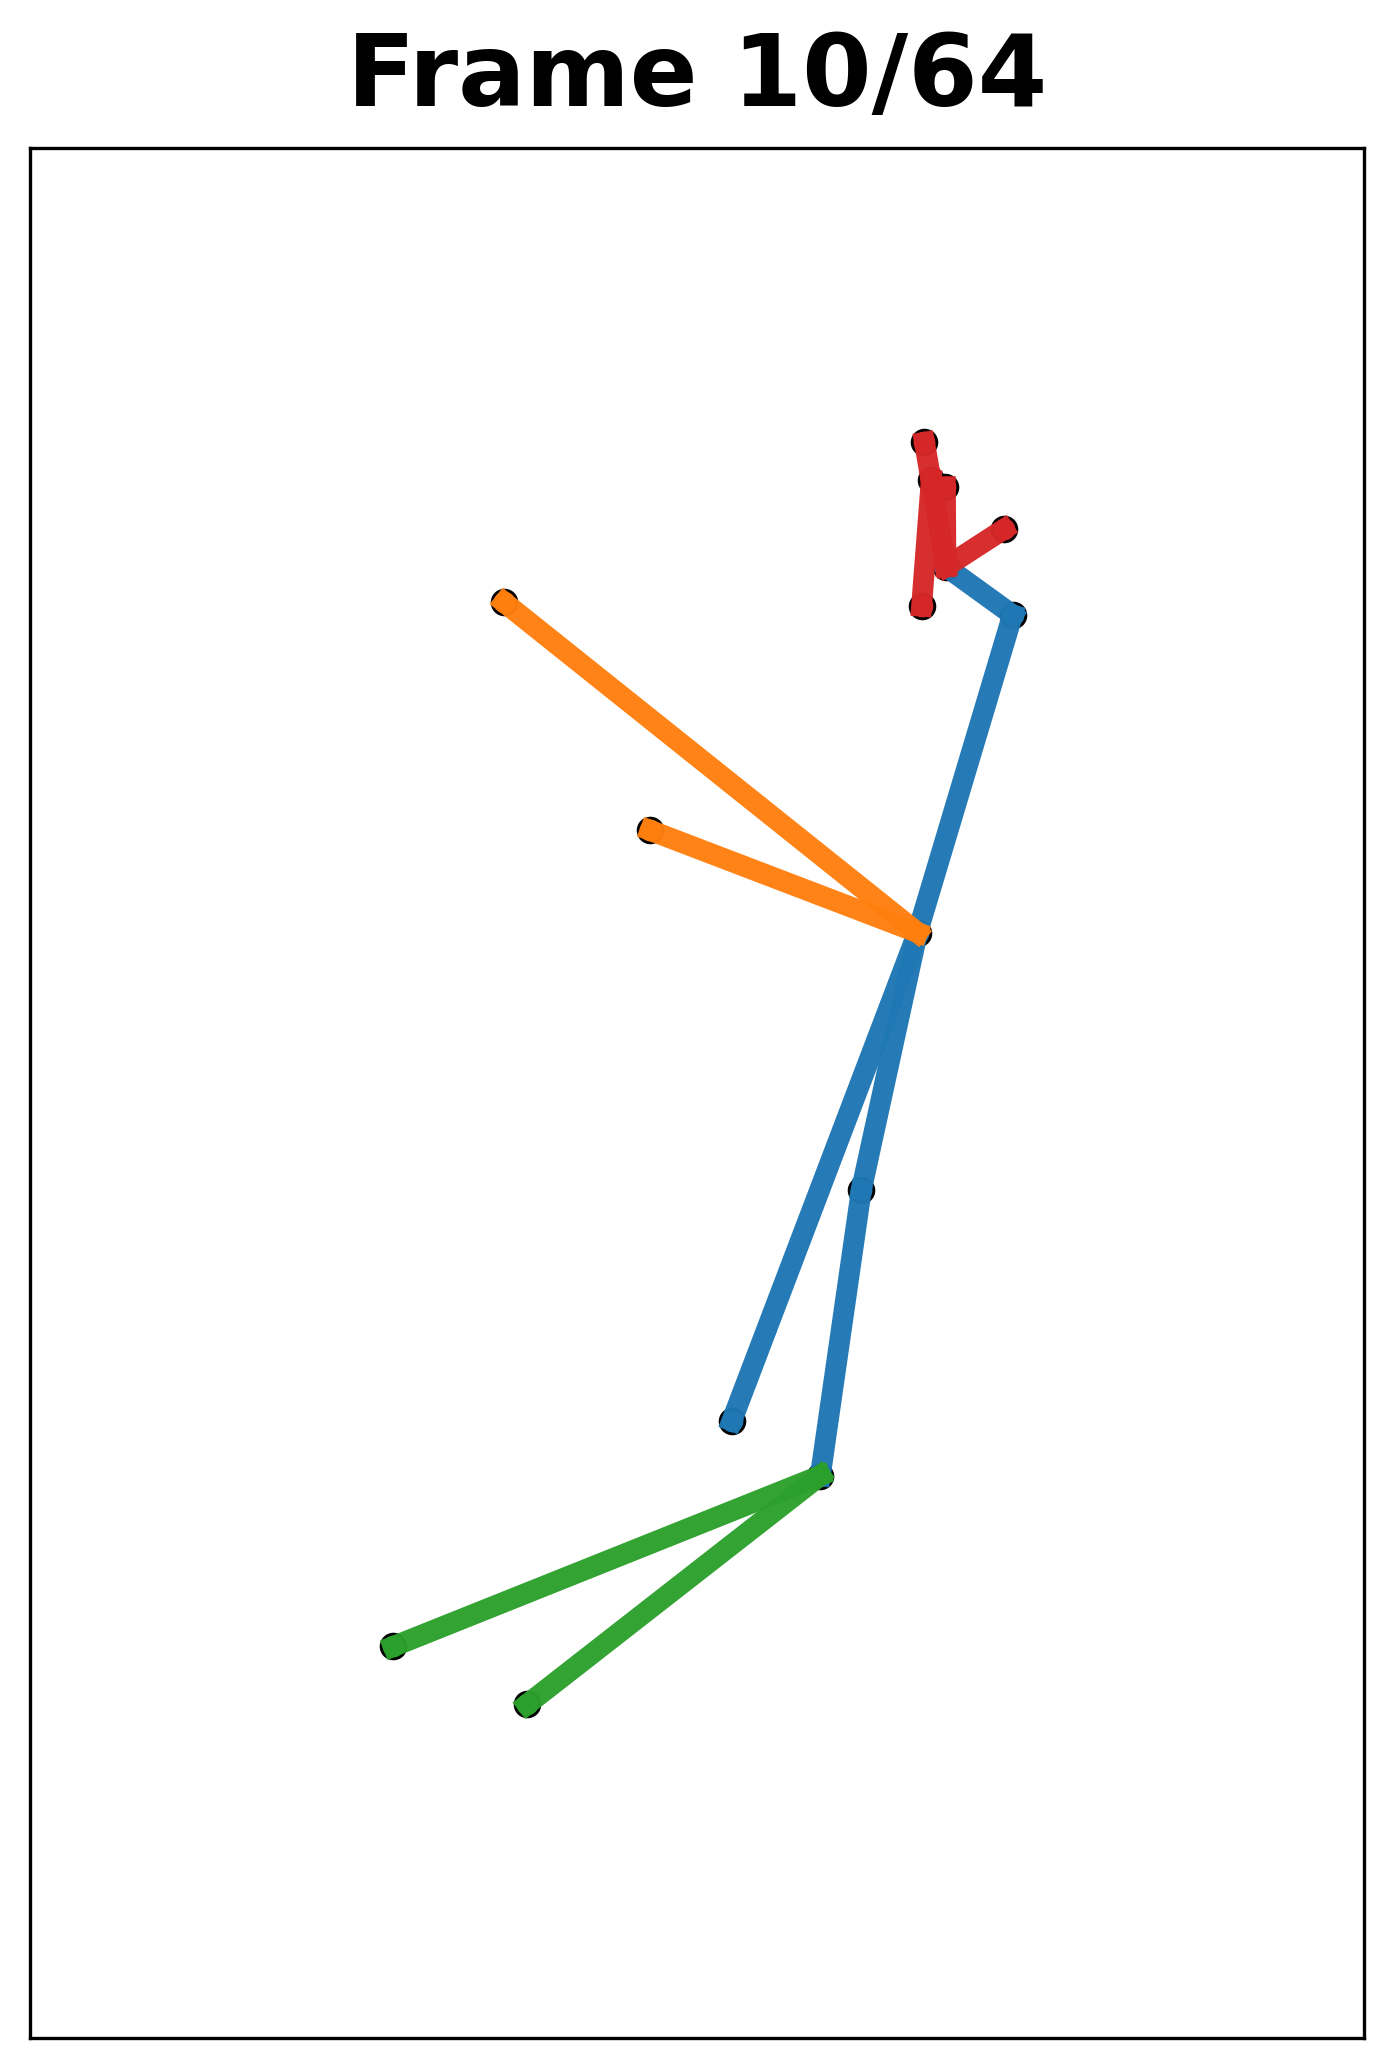
\includegraphics[width=\linewidth]{figures/ReportFigures/frame_010.png}
%   \caption{}
%   \label{fig:r1c1}
% \end{subfigure}\hfill
% \begin{subfigure}[t]{0.19\textwidth}
%   \centering
%   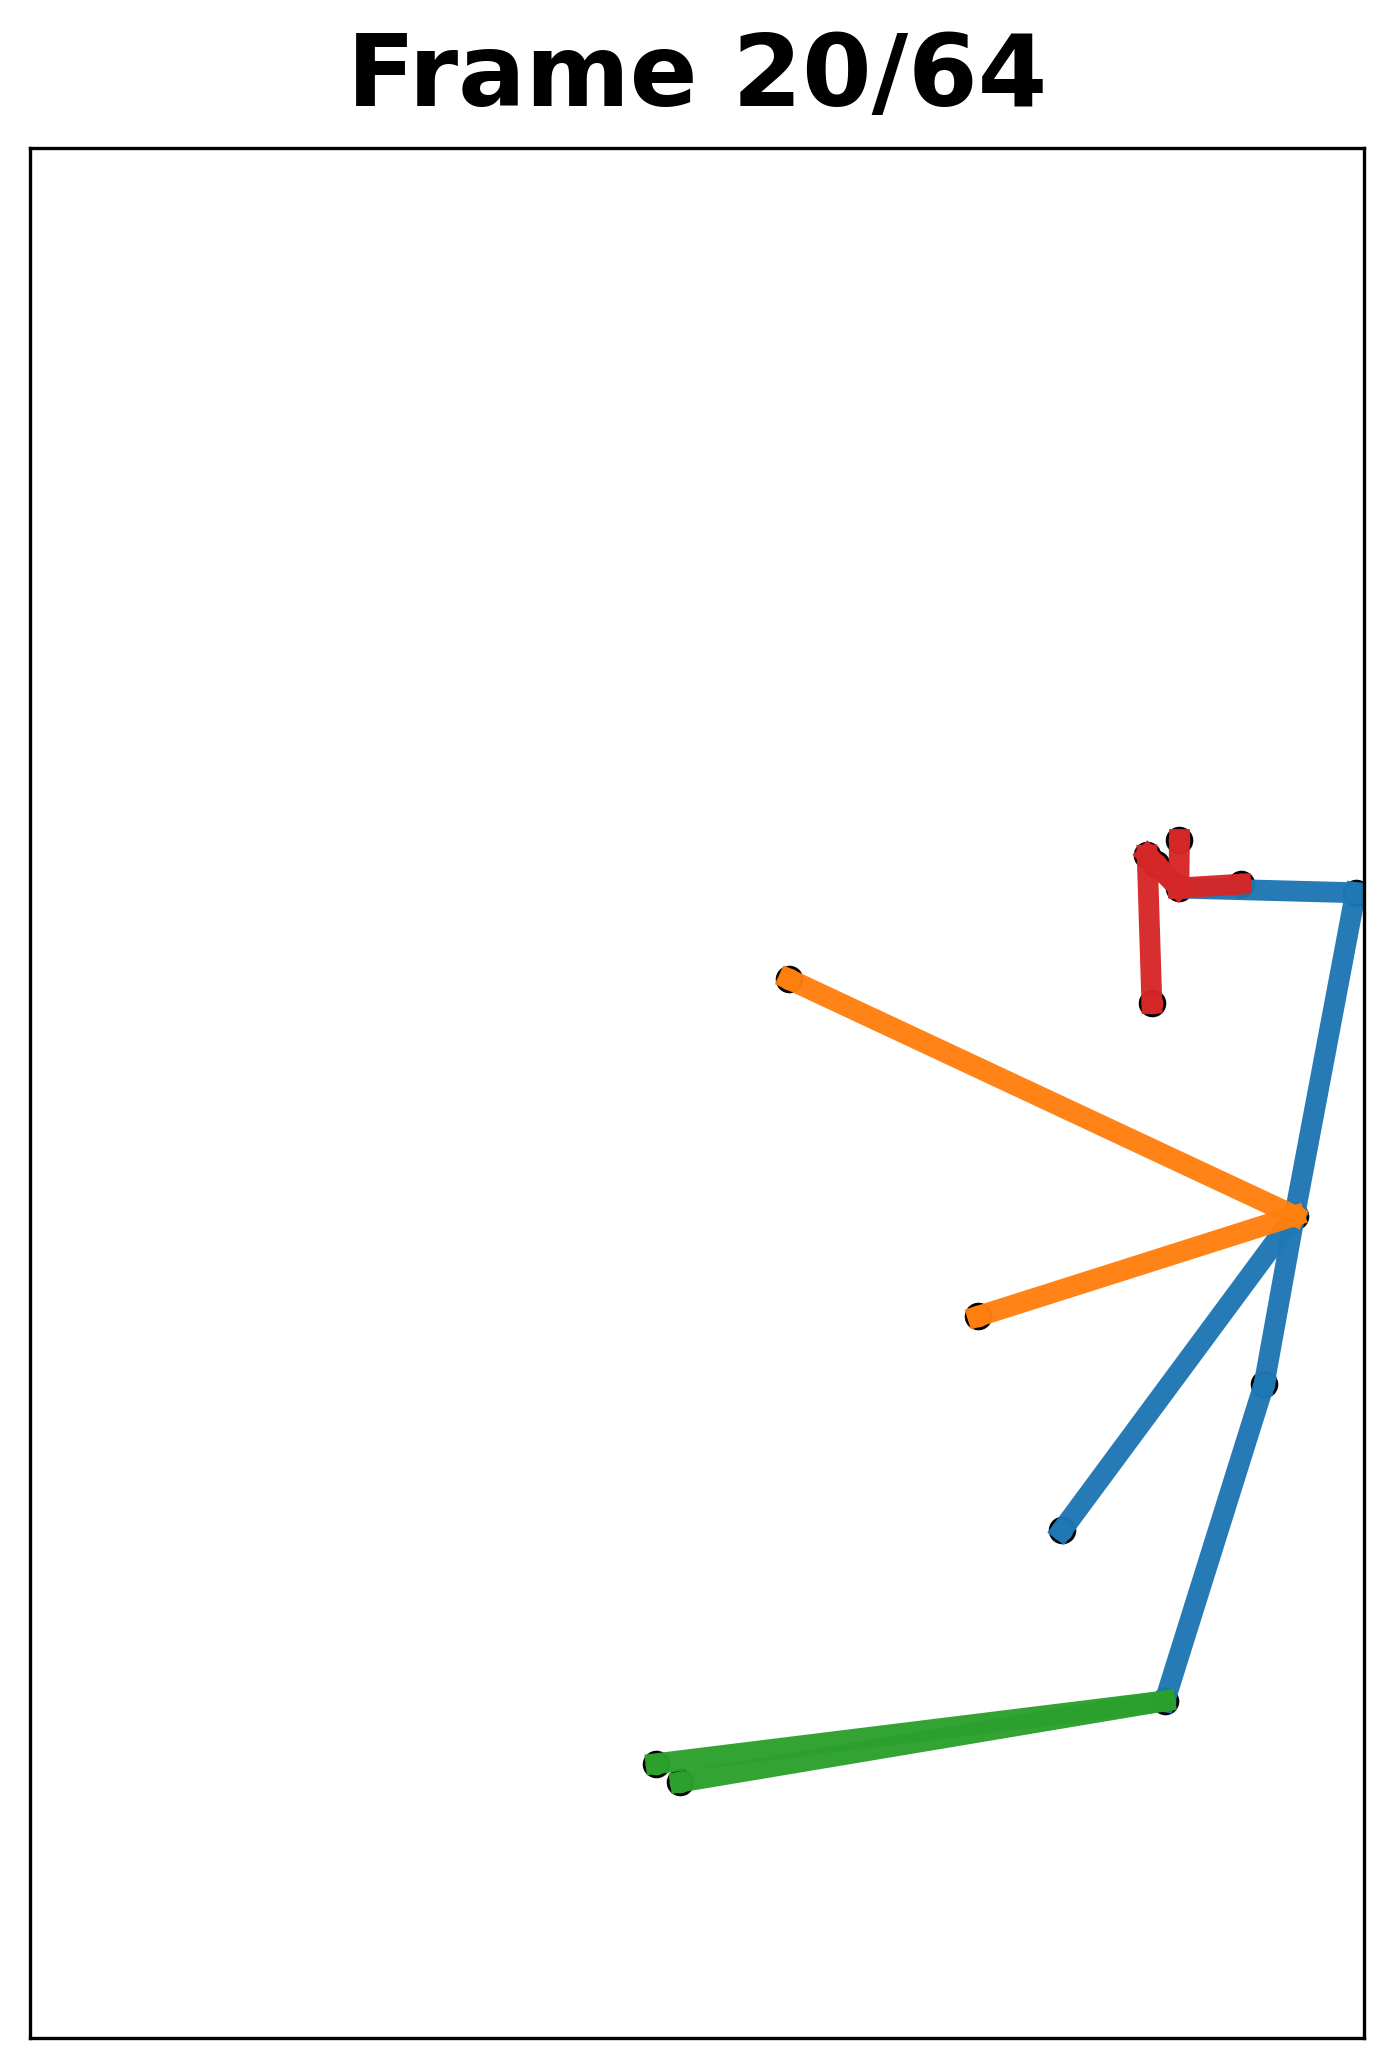
\includegraphics[width=\linewidth]{figures/ReportFigures/frame_020.png}
%   \caption{}
%   \label{fig:r1c2}
% \end{subfigure}\hfill
% \begin{subfigure}[t]{0.19\textwidth}
%   \centering
%   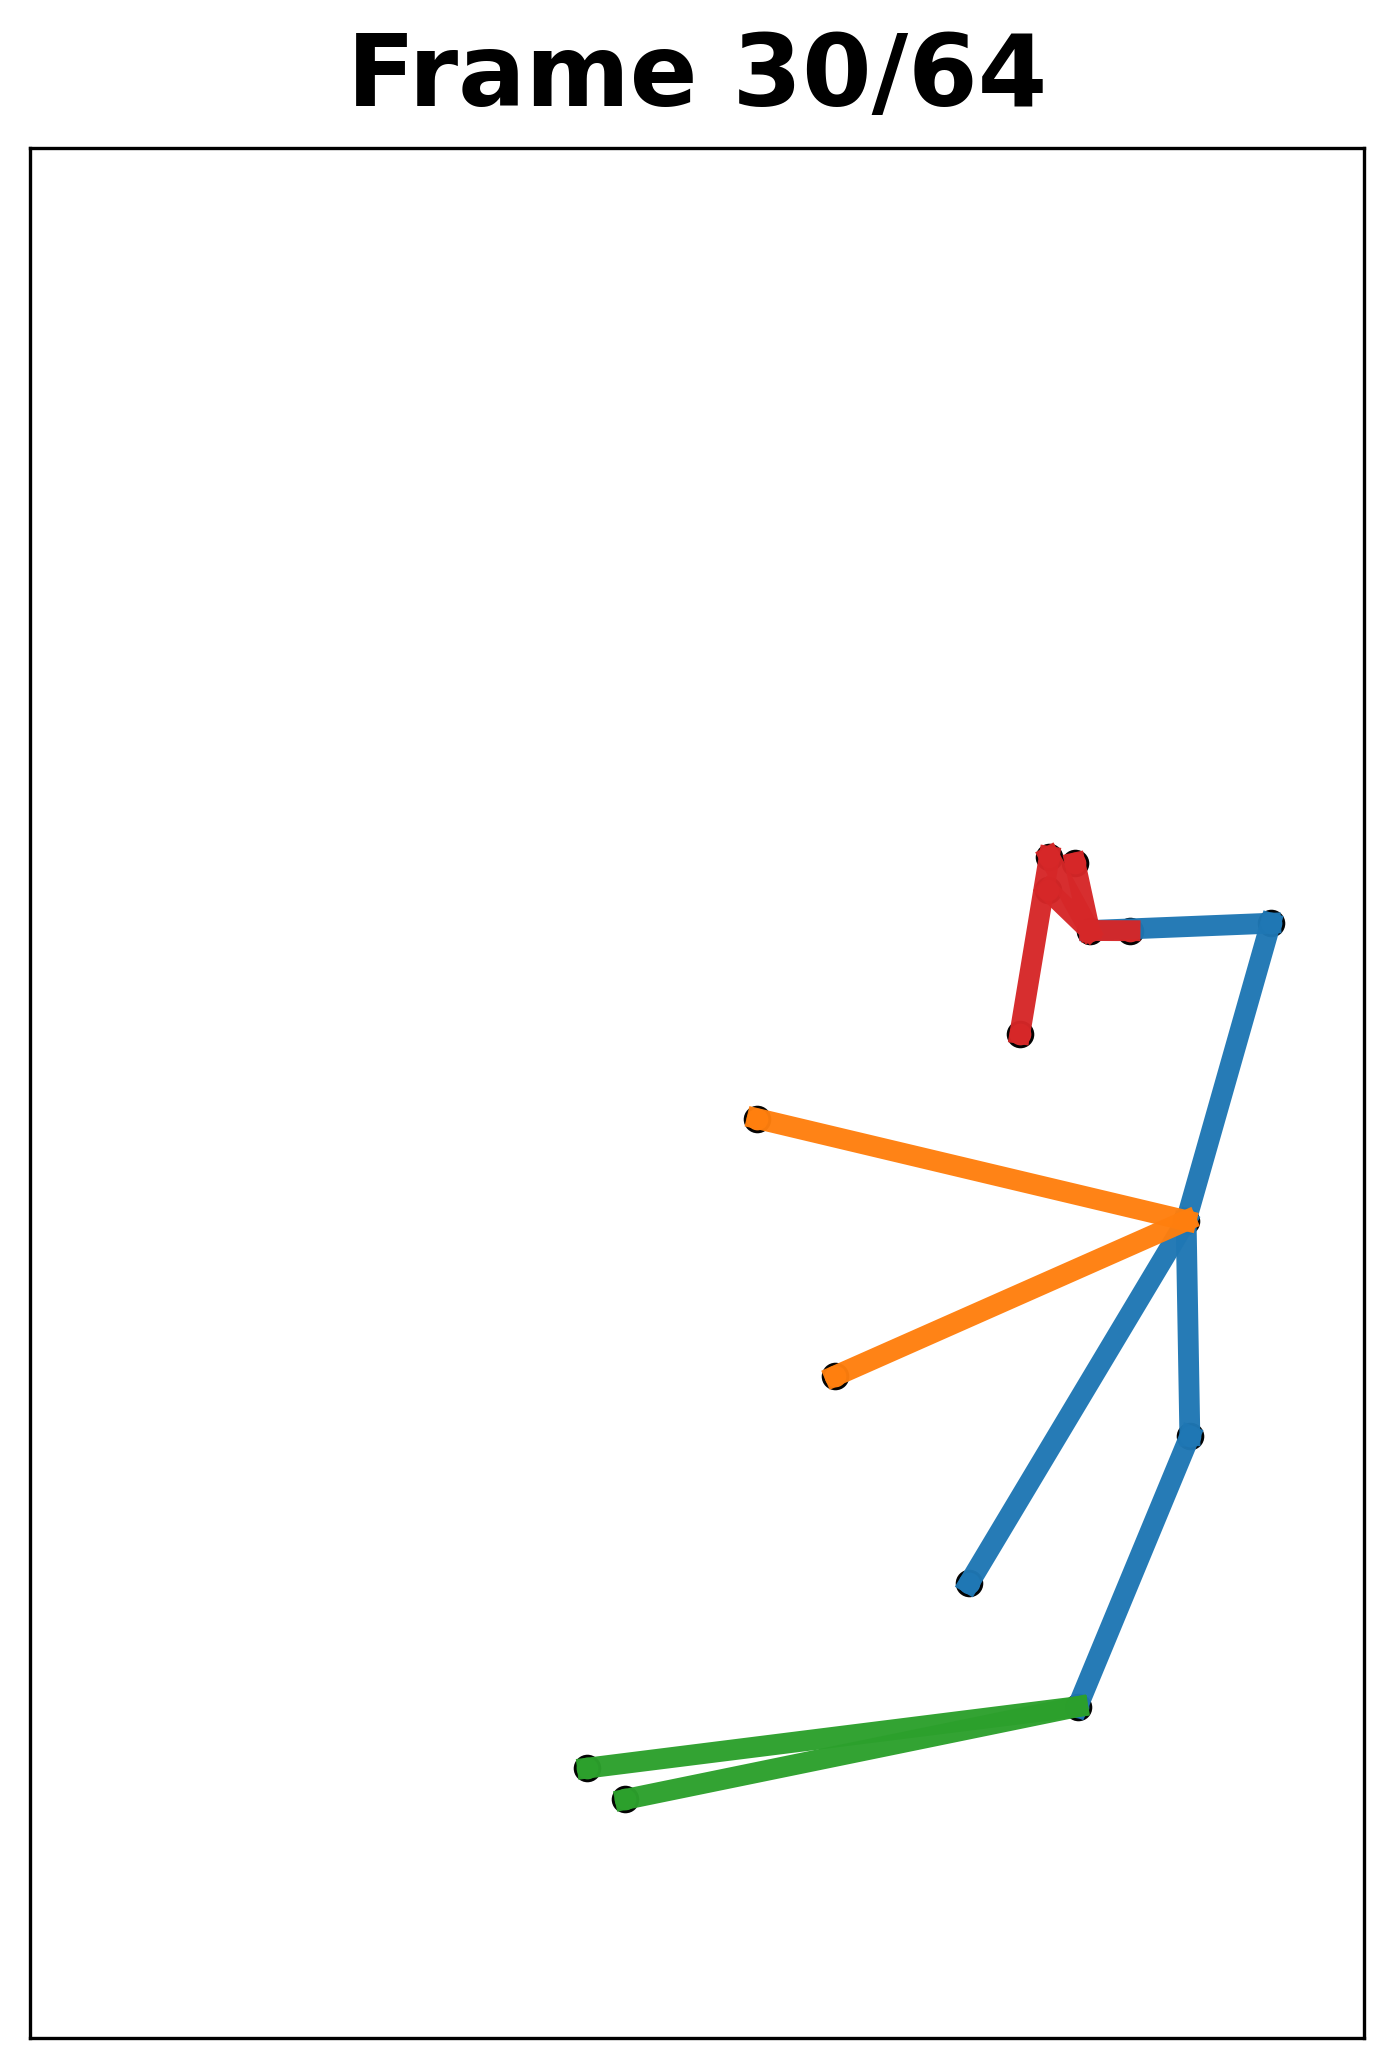
\includegraphics[width=\linewidth]{figures/ReportFigures/frame_030.png}
%   \caption{}
%   \label{fig:r1c3}
% \end{subfigure}\hfill
% \begin{subfigure}[t]{0.19\textwidth}
%   \centering
%   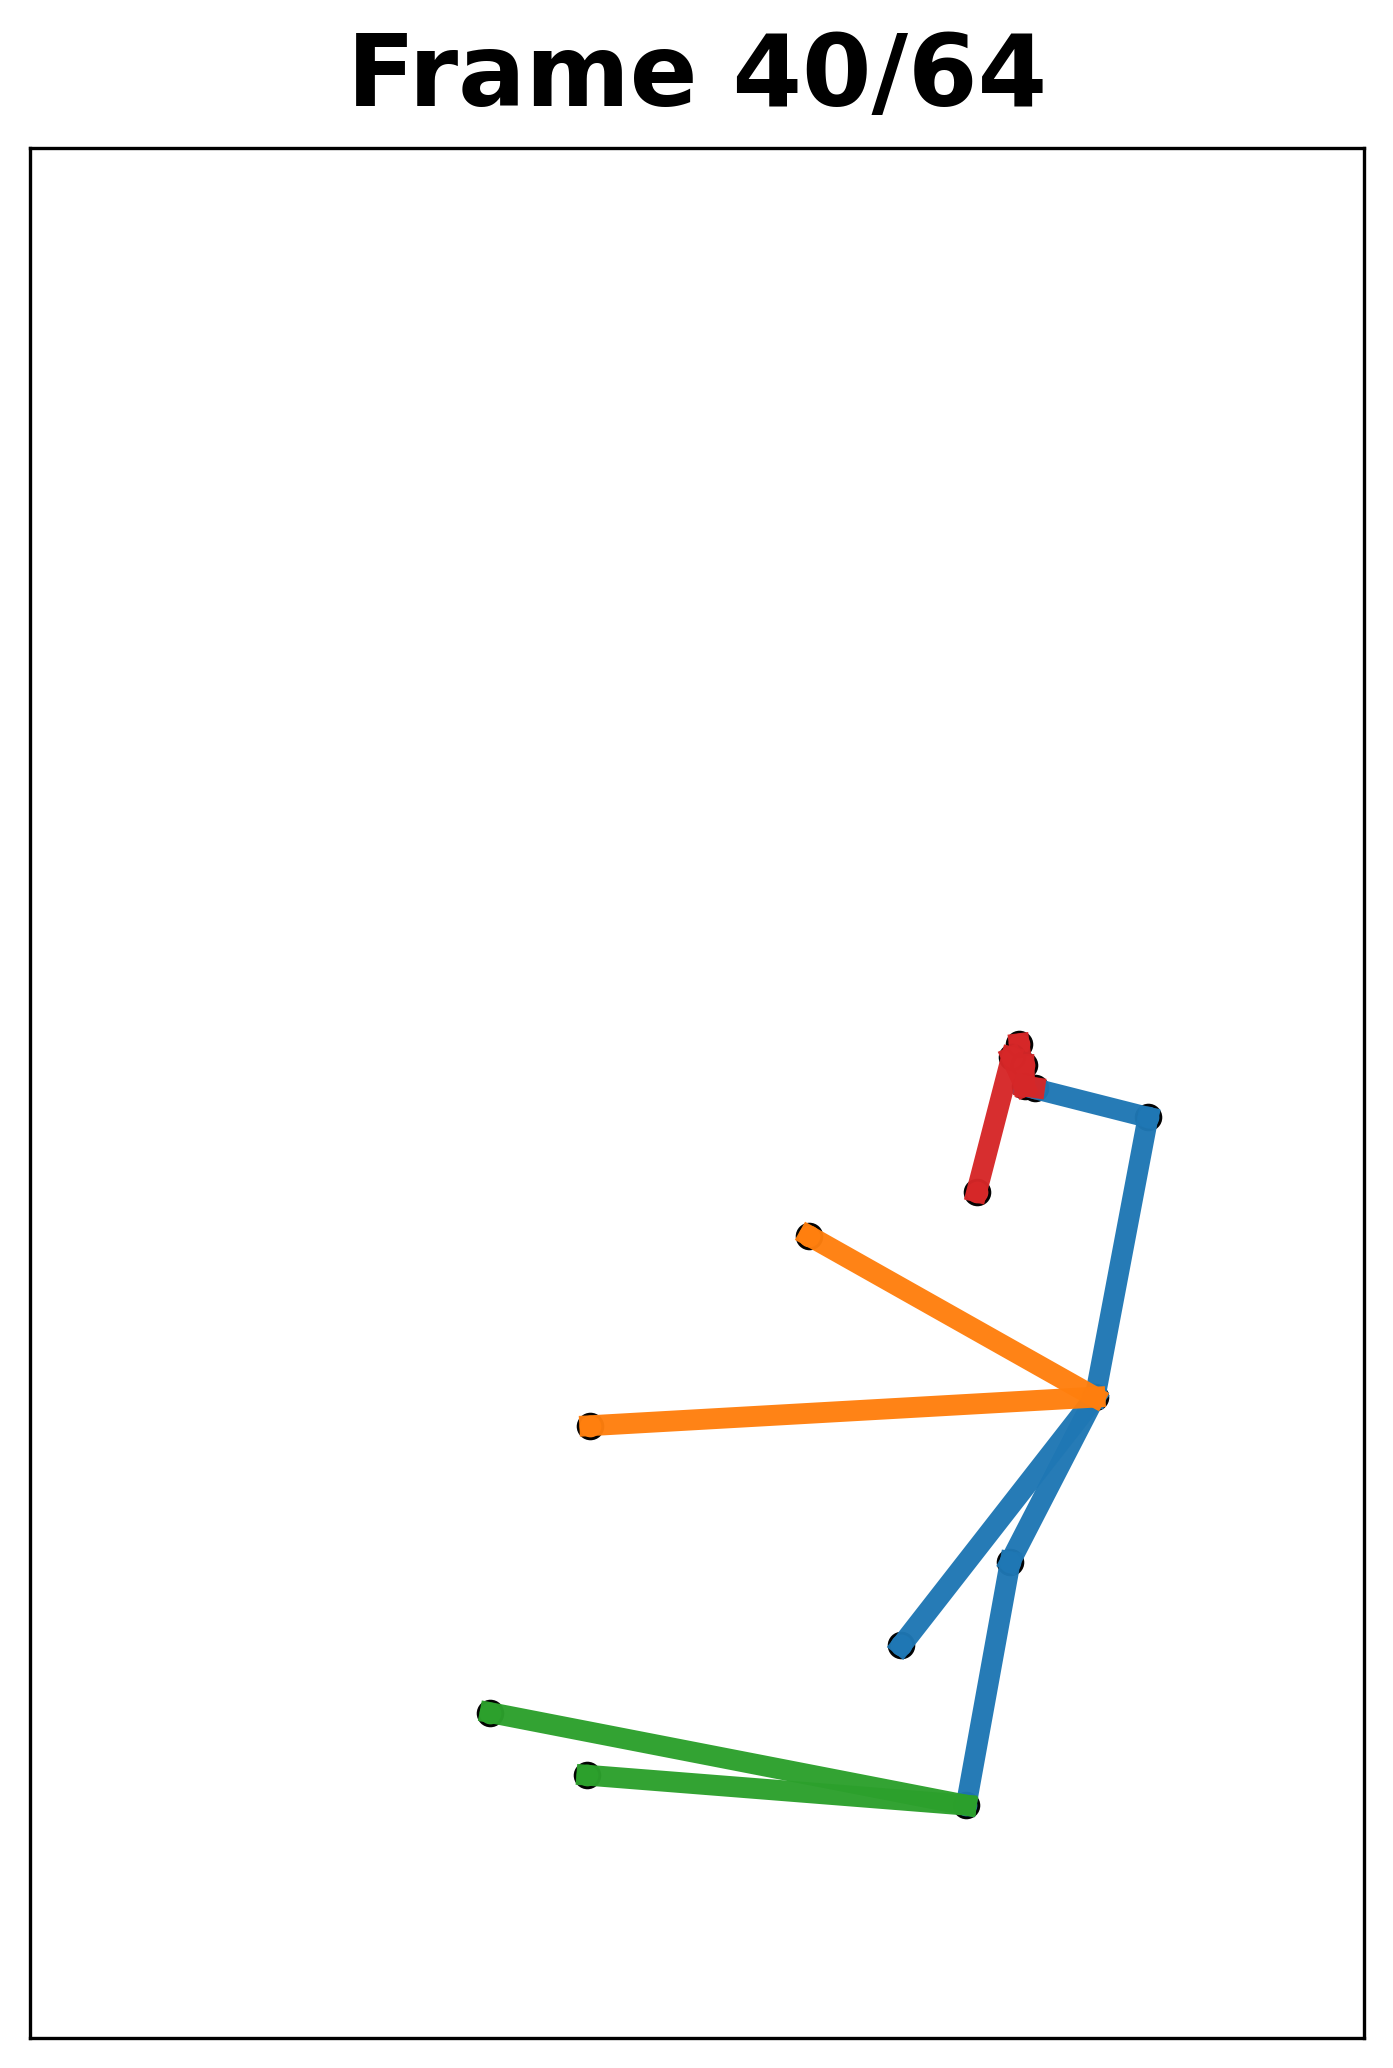
\includegraphics[width=\linewidth]{figures/ReportFigures/frame_040.png}
%   \caption{}
%   \label{fig:r1c4}
% \end{subfigure}\hfill
% \begin{subfigure}[t]{0.19\textwidth}
%   \centering
%   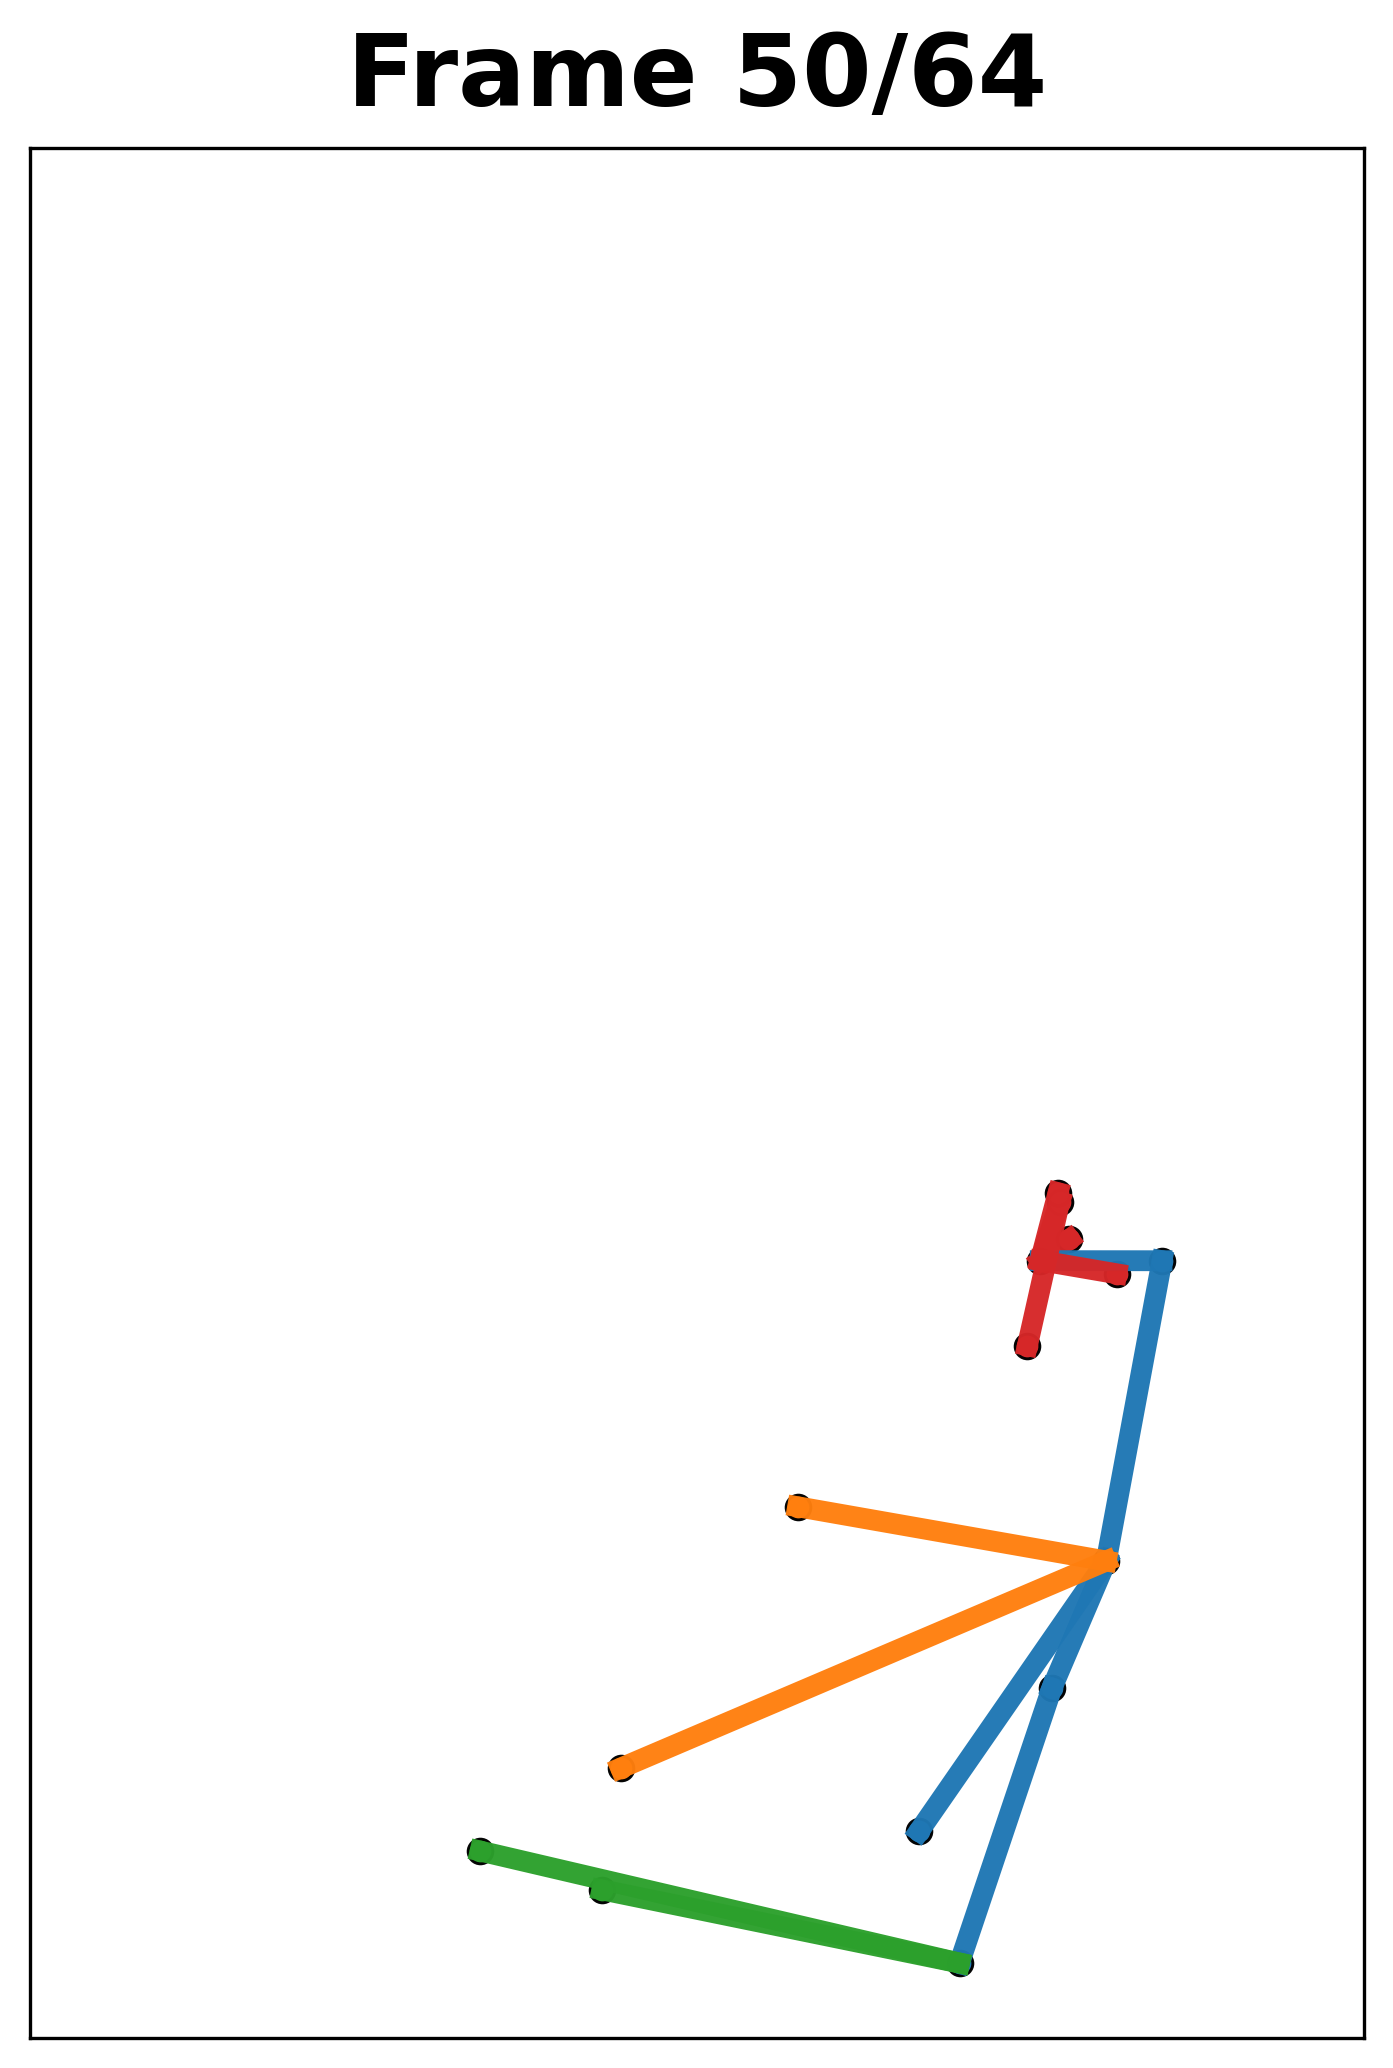
\includegraphics[width=\linewidth]{figures/ReportFigures/frame_050.png}
%   \caption{}
%   \label{fig:r1c5}
% \end{subfigure}

% \vspace{0.6em}

% % ---------- Row 2 ----------
% \begin{subfigure}[t]{0.19\textwidth}
%   \centering
%   \includegraphics[width=\linewidth]{figures/ReportFigures/glidingframe_010.png}
%   \caption{}
%   \label{fig:r2c1}
% \end{subfigure}\hfill
% \begin{subfigure}[t]{0.19\textwidth}
%   \centering
%   \includegraphics[width=\linewidth]{figures/ReportFigures/glidingframe_020.png}
%   \caption{}
%   \label{fig:r2c2}
% \end{subfigure}\hfill
% \begin{subfigure}[t]{0.19\textwidth}
%   \centering
%   \includegraphics[width=\linewidth]{figures/ReportFigures/glidingframe_030.png}
%   \caption{}
%   \label{fig:r2c3}
% \end{subfigure}\hfill
% \begin{subfigure}[t]{0.19\textwidth}
%   \centering
%   \includegraphics[width=\linewidth]{figures/ReportFigures/glidingframe_040.png}
%   \caption{}
%   \label{fig:r2c4}
% \end{subfigure}\hfill
% \begin{subfigure}[t]{0.19\textwidth}
%   \centering
%   \includegraphics[width=\linewidth]{figures/ReportFigures/glidingframe_050.png}
%   \caption{}
%   \label{fig:r2c5}
% \end{subfigure}

% \vspace{0.6em}

% % ---------- Row 3 ----------
% \begin{subfigure}[t]{0.19\textwidth}
%   \centering
%   \includegraphics[width=\linewidth]{figures/ReportFigures/hoveringframe_010.png}
%   \caption{}
%   \label{fig:r3c1}
% \end{subfigure}\hfill
% \begin{subfigure}[t]{0.19\textwidth}
%   \centering
%   \includegraphics[width=\linewidth]{figures/ReportFigures/hoveringframe_020.png}
%   \caption{}
%   \label{fig:r3c2}
% \end{subfigure}\hfill
% \begin{subfigure}[t]{0.19\textwidth}
%   \centering
%   \includegraphics[width=\linewidth]{figures/ReportFigures/hoveringframe_030.png}
%   \caption{}
%   \label{fig:r3c3}
% \end{subfigure}\hfill
% \begin{subfigure}[t]{0.19\textwidth}
%   \centering
%   \includegraphics[width=\linewidth]{figures/ReportFigures/hoveringframe_040.png}
%   \caption{}
%   \label{fig:r3c4}
% \end{subfigure}\hfill
% \begin{subfigure}[t]{0.19\textwidth}
%   \centering
%   \includegraphics[width=\linewidth]{figures/ReportFigures/hoveringframe_050.png}
%   \caption{}
%   \label{fig:r3c5}
% \end{subfigure}

% \caption{Overall caption for the 3$\times$5 grid.}
% \label{fig:grid3x5}
% \end{figure}







% \begin{figure}[htbp]
%     \centering
    
%     % 第一张图片
%     \begin{subfigure}[t]{0.15\textwidth}
%         \centering
%         \includegraphics[width=\textwidth]{figures/Fig2-1.png}
%         \caption{}
%         \label{fig2-1}
%     \end{subfigure}
%     \hspace{1em}
%     % 第二张图片
%     \begin{subfigure}[t]{0.15\textwidth}
%         \centering
%         \includegraphics[width=\textwidth]{figures/Fig2-2.png}
%         \caption{}
%         \label{fig:gen_frame2}
%     \end{subfigure}
%     \hspace{0.1em}
%     % 第三张图片
%     \begin{subfigure}[t]{0.15\textwidth}
%         \centering
%         \includegraphics[width=\textwidth]{figures/Fig2-3.png}
%         \caption{}
%         \label{fig:gen_frame3}
%     \end{subfigure}
%     \hspace{0.1em}
%     % 第四张图片
%     \begin{subfigure}[t]{0.15\textwidth}
%         \centering
%         \includegraphics[width=\textwidth]{figures/Fig2-4.png}
%         \caption{}
%         \label{fig:gen_frame4}
%     \end{subfigure}
%     \hspace{0.1em}
%     % 第五张图片
%     \begin{subfigure}[t]{0.15\textwidth}
%         \centering
%         \includegraphics[width=\textwidth]{figures/Fig2-5.png}
%         \caption{}
%         \label{fig:gen_frame5}
%     \end{subfigure}
%     \hspace{0.1em}
%     % 第六张图片
%     \begin{subfigure}[t]{0.15\textwidth}
%         \centering
%         \includegraphics[width=\textwidth]{figures/Fig2-6.png}
%         \caption{}
%         \label{fig:gen_frame6}
%     \end{subfigure}
    
%     \caption{\centering Video frame generated using the base AnimateDiff pipeline.\\
% (a) Initial image generated with Stable Diffusion, used as the input of video generation.\\ (b-f) Frames sampled from a 24-frame video generation using 2(a) as the initial frame.}
%     \label{fig:frame_comparison_1}
% \end{figure}

% \begin{figure}[htbp]
%     \centering
    
%     % 第一张图片
%     \begin{subfigure}[t]{0.15\textwidth}
%         \centering
%         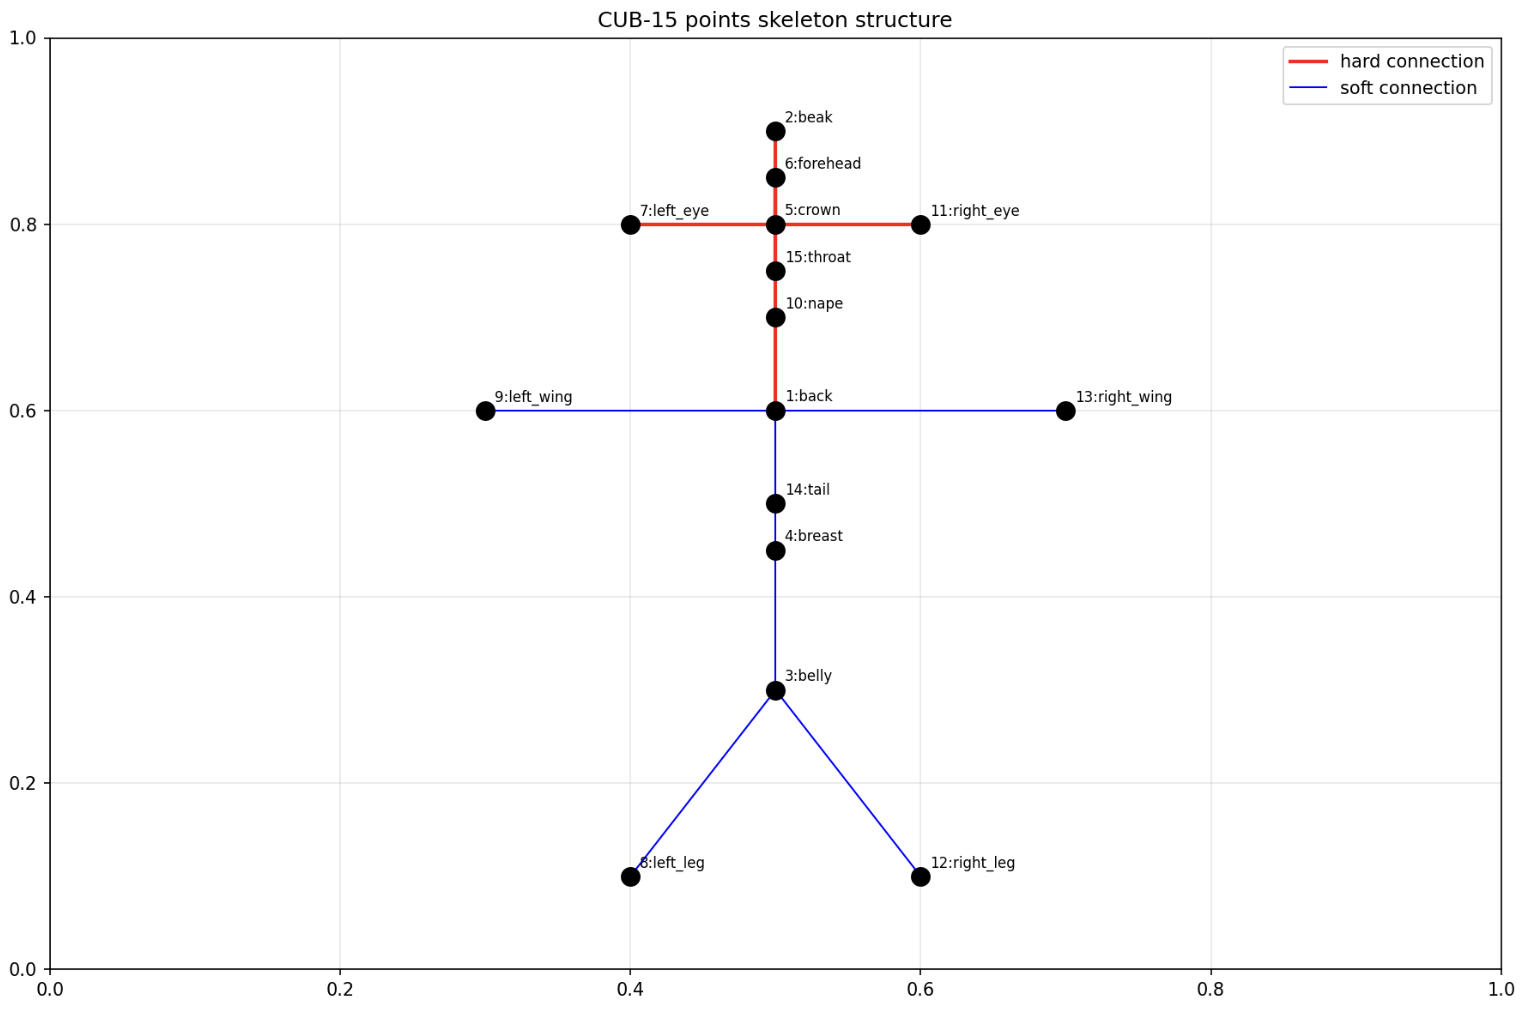
\includegraphics[width=\textwidth]{figures/Fig1-1.png}
%         \caption{}
%         \label{fig1-1}
%     \end{subfigure}
%     \hspace{1em}
%     % 第二张图片
%     \begin{subfigure}[t]{0.15\textwidth}
%         \centering
%         \includegraphics[width=\textwidth]{figures/Fig1-2.png}
%         \caption{}
%         \label{fig:gen_frame2}
%     \end{subfigure}
%     \hspace{0.1em}
%     % 第三张图片
%     \begin{subfigure}[t]{0.15\textwidth}
%         \centering
%         \includegraphics[width=\textwidth]{figures/Fig1-3.png}
%         \caption{}
%         \label{fig:gen_frame3}
%     \end{subfigure}
%     \hspace{0.1em}
%     % 第四张图片
%     \begin{subfigure}[t]{0.15\textwidth}
%         \centering
%         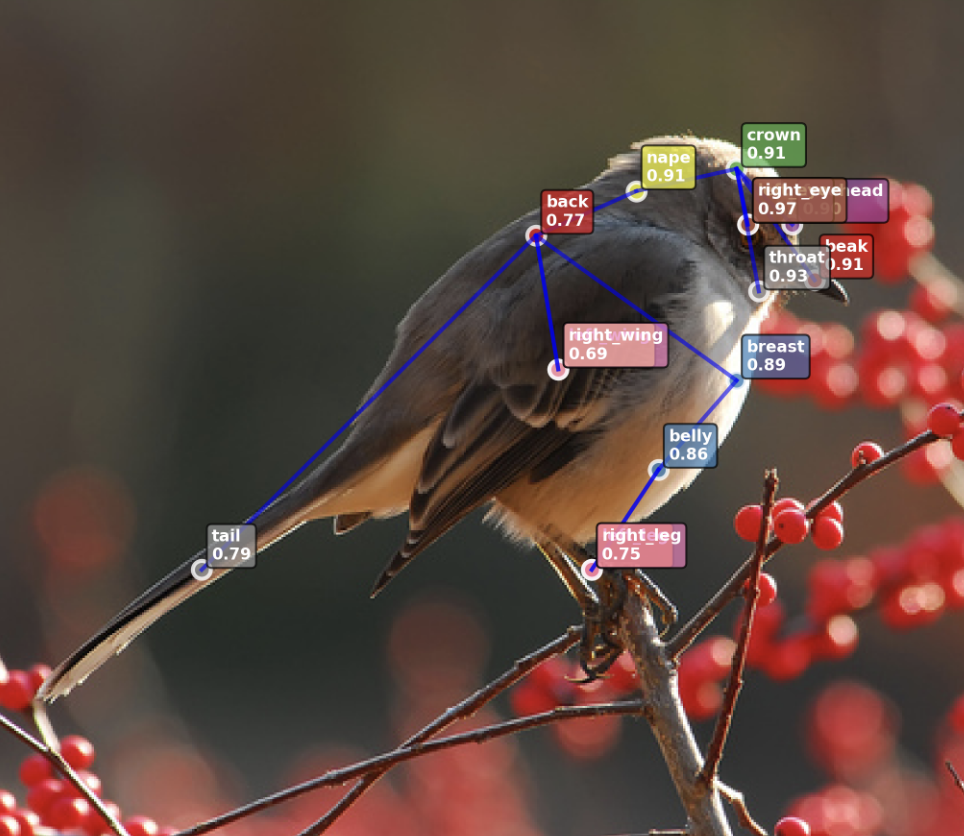
\includegraphics[width=\textwidth]{figures/Fig1-4.png}
%         \caption{}
%         \label{fig:gen_frame4}
%     \end{subfigure}
%     \hspace{0.1em}
%     % 第五张图片
%     \begin{subfigure}[t]{0.15\textwidth}
%         \centering
%         \includegraphics[width=\textwidth]{figures/Fig1-5.png}
%         \caption{}
%         \label{fig:gen_frame5}
%     \end{subfigure}
%     \hspace{0.1em}
%     % 第六张图片
%     \begin{subfigure}[t]{0.15\textwidth}
%         \centering
%         \includegraphics[width=\textwidth]{figures/Fig1-6.png}
%         \caption{}
%         \label{fig:gen_frame6}
%     \end{subfigure}
    
%     \caption{\centering Video frame comparison using AnimateDiff with ControlNet.\\
% (a) Initial image generated with Stable Diffusion, used as the input of video generation.\\ (b-f) Frames sampled from a 24-frame video generation sing 3(a) as the initial frame.}
%     \label{fig:frame_comparison_2}
% \end{figure}


% \section{Expected Outcomes and Deliverables}
% The project will produce a combination of technical, experimental, and optional creative outputs:
% \begin{itemize}
%     \item A modular video synthesis pipeline for surreal bird imagery, built on AnimateDiff with ControlNet and LoRA integration, ensuring temporal consistency in generated sequences.
%     \item An annotated dataset of surreal bird videos documenting experimental parameters (conditioning methods, schedulers, attention mechanisms) for research reuse.
%     \item Comparative experimental findings on temporal coherence, feature retention, and conditioning efficacy, combining quantitative metrics with qualitative assessment.
%     \item Complete MSc research documentation with technical report and well-documented code repository.
%     \item Series of exhibition-ready visual outputs with critical commentary.
% \end{itemize}





% \section{Future plan}
% % Figure
% \begin{figure}[H]
%     \begin{center}
%         \includegraphics[width=0.9\textwidth]{plan.jpg}
%     \end{center}
%     \caption{\label{fig:plan} Research timeline}
% \end{figure}
% \resizebox{\textwidth}{!}{
% \begin{ganttchart}[
%   hgrid style/.style={black, dotted},
%   vgrid style/.style={black!20!white},
%   x unit=2.3mm,
%   y unit chart=9mm,
%   y unit title=10mm,
%   time slot format=isodate,
%   compress calendar,
%   group label font=\bfseries\small,
%   milestone label font=\bfseries\small,
%   bar label font=\normalsize\slshape,
%   bar height=0.6,
%   bar/.append style={fill=pyblue},
%   link/.style={->, thick}
% ]{2025-05-26}{2025-08-29}
% \gantttitlecalendar{year, month=name, week}\\

% \ganttbar[bar/.append style={fill=moryellow}]{Setup HPC and AnimateDiff}{2025-05-26}{2025-06-06} \\
% \ganttbar[bar/.append style={fill=morblue}]{Literature + dataset prep}{2025-05-26}{2025-06-06} \\
% \ganttbar[bar/.append style={fill=morblue}]{Write Project Report}{2025-05-30}{2025-06-13} \\
% \ganttbar[bar/.append style={fill=moryellow}]{Baseline: AnimateDiff + RealisticVision}{2025-06-02}{2025-06-09} \\
% \ganttbar[bar/.append style={fill=morgreen}]{Phase 1: Normal → Normal bird video}{2025-06-09}{2025-06-16} \\
% \ganttbar[bar/.append style={fill=morgreen}]{Phase 2: Surreal → Surreal bird video}{2025-06-16}{2025-06-27} \\
% \ganttbar[bar/.append style={fill=morrose}]{LoRA fine-tuning (motion, attention)}{2025-06-30}{2025-07-17} \\
% \ganttbar[bar/.append style={fill=morrose}]{Saliency eccentricity tracking}{2025-06-30}{2025-07-17} \\
% \ganttbar[bar/.append style={fill=morrose}]{Temporal consistency (DDIM, attention)}{2025-07-01}{2025-07-19} \\
% \ganttbar[bar/.append style={fill=morgreen}]{Phase 3: Normal → Surreal → Video}{2025-07-15}{2025-07-26} \\
% \ganttbar[bar/.append style={fill=morgreen}]{Phase 4: Fully surreal motion videos}{2025-07-26}{2025-08-02} \\
% \ganttbar[bar/.append style={fill=moryellow}]{Evaluation (FVD, CLIP drift)}{2025-08-02}{2025-08-09} \\
% \ganttbar[bar/.append style={fill=morblue}]{Report writing}{2025-08-09}{2025-08-29}
% \end{ganttchart}
% }


% \resizebox{\textwidth}{!}{
% \begin{ganttchart}[
%   hgrid style/.style={black, dotted},
%   vgrid style/.style={black!20!white},
%   x unit=2.3mm,
%   y unit chart=9mm,
%   y unit title=10mm,
%   time slot format=isodate,
%   compress calendar,
%   group label font=\bfseries\small,
%   milestone label font=\bfseries\small,
%   bar label font=\normalsize\slshape,
%   bar height=0.6,
%   bar/.append style={fill=pyblue},
%   link/.style={->, thick}
% ]{2025-05-26}{2025-08-29}

% \gantttitlecalendar{year, month=name, week}\\

% % Week 1-2: Initial Setup
% \ganttbar[bar/.append style={fill=morbrown}]{Setup HPC and AnimateDiff}{2025-05-26}{2025-06-06} \\
% \ganttbar[bar/.append style={fill=morbrown}]{Literature + dataset prep}{2025-05-26}{2025-06-06} \\

% % Week 2-4: Dataset Preparation & Planning
% \ganttbar[bar/.append style={fill=morpurple}]{Dataset preparation (CUB-200, VB100, FBD-SV)}{2025-06-02}{2025-06-20} \\
% \ganttbar[bar/.append style={fill=morpurple}]{Surreal bird generation (GPT API)}{2025-06-02}{2025-06-20} \\
% \ganttbar[bar/.append style={fill=morpurple}]{Write Project Report}{2025-06-02}{2025-06-13} \\

% % Week 4-5: Baseline & ControlNet Prep
% \ganttbar[bar/.append style={fill=moryellow}]{Phase 1: Baseline (AnimateDiff + RealisticVision)}{2025-06-16}{2025-06-27} \\
% \ganttbar[bar/.append style={fill=moryellow}]{Phase 2: ControlNet integration prep}{2025-06-20}{2025-06-27} \\

% % Week 5-6: Phase 2 Implementation
% \ganttbar[bar/.append style={fill=morgreen}]{Phase 2: ControlNet integration}{2025-06-23}{2025-07-04} \\
% \ganttbar[bar/.append style={fill=morgreen}]{Guided synthesis + structural coherence}{2025-06-23}{2025-07-04} \\

% % Week 6-8: Phase 3 Feature Preservation
% \ganttbar[bar/.append style={fill=morred}]{Phase 3: 
% Low-Rank Noise Projection (PyoCo)}{2025-06-30}{2025-07-18} \\
% \ganttbar[bar/.append style={fill=morred}]{CLIP-guided semantic consistency}{2025-06-30}{2025-07-18} \\
% \ganttbar[bar/.append style={fill=morred}]{Enhanced feature retention}{2025-06-30}{2025-07-18} \\

% % Week 7-9: Phase 4 Temporal Optimization (Overlapping with Phase 3)
% \ganttbar[bar/.append style={fill=morblue!50}]{Phase 4: Sampling schedulers (DDIM vs DDPM)}{2025-07-07}{2025-07-25} \\
% \ganttbar[bar/.append style={fill=morblue!50}]{Temporal attention module}{2025-07-07}{2025-07-25} \\
% \ganttbar[bar/.append style={fill=morblue!50}]{Latent space consistency + noise reduction}{2025-07-07}{2025-07-25} \\

% % Week 9-11: Phase 5 Final Video Generation
% \ganttbar[bar/.append style={fill=mororange}]{Phase 5: Normal→Surreal transitions}{2025-07-21}{2025-08-08} \\
% \ganttbar[bar/.append style={fill=mororange}]{Fully surreal motion videos}{2025-07-21}{2025-08-08} \\

% % Week 10-12: Evaluation (Overlapping with Phase 5)
% \ganttbar[bar/.append style={fill=moryellow}]{Evaluation (FVD, CLIP drift)}{2025-08-04}{2025-08-22} \\

% % Week 12-14: Analysis & Report Writing (Overlapping with Evaluation)
% \ganttbar[bar/.append style={fill=morblue}]{Performance analysis \& report writing}{2025-08-08}{2025-08-29}

% \end{ganttchart}
% }

% References
% \newpage

% \section*{AI Acknowledgment}
% \begin{itemize}
%     \item \textbf{Tool Name and Version}: ChatGPT (4o)
%     \item \textbf{Publisher/Provider}: OpenAI
%     \item \textbf{URL}: https://chatgpt.com/?model=gpt-4o
%     \item \textbf{Usage Description}: ChatGPT was used in the initial research phase to analyze project requirements, understand AI frameworks by clarifying documentation and simplifying explanations, and provide guidance on environment setup and resolving module issues during HPC deployment.
%     \item \textbf{Declaration}: All submitted work is my own. AI tools were used solely to support the development and understanding of the project, not to generate final content.
% \end{itemize}


\subsection{Video Generation using AnimateDiffusion + ControlNet
}
\subsubsection{Qualitative results with CUB-15 skeletons}

% The qualitative results demonstrate that the proposed skeleton-guided pipeline effectively generates temporally coherent bird motion videos, while simultaneously preserving both realistic and surreal visual traits. Across test sequences, the generated outputs closely follow the provided skeleton trajectories, with wing flapping, body orientation, and flight dynamics remaining consistent over time. This highlights the strong controllability of the framework and its ability to disentangle appearance from motion.

% The impact of different ControlNet conditioning signals is evident. Canny edges preserve global silhouettes and prevent structural drifting, while depth maps enhance volumetric perception by introducing three-dimensional cues. OpenPose-style skeletons contribute most significantly to frame-to-frame consistency, ensuring that local motion trajectories remain aligned with the input skeleton sequence. Together, these complementary constraints achieve a balance between visual fidelity and motion control.

% For the realistic bird example, varying the relative weights of ControlNet inputs produces distinct trade-offs. Higher pose weights yield motions that more strictly follow the skeleton, though sometimes at the expense of fine appearance details. Conversely, stronger edge signals sharpen contours but may reduce adherence to the skeleton. For the surreal purple bird case, the system successfully preserves unnatural color patterns and morphology while maintaining smooth motion, confirming that the method supports creative extrapolation beyond naturalistic appearances.

% Despite these successes, limitations remain. Excessive reliance on skeleton constraints occasionally suppresses high-frequency details such as feather textures, and different ControlNet branches require empirical tuning to avoid imbalances. In some outputs, subtle drifting and imperfect background integration are observed. Nonetheless, the results validate that the AnimateDiff + ControlNet integration provides an effective compromise between controllability, temporal smoothness, and surreal trait preservation.


Generated sequences based on CUB-15 skeletons exhibit temporally coherent motion while preserving both realistic and surreal traits. 
Across test cases, outputs closely follow the provided skeleton trajectories, with wing flapping, body orientation, and overall flight dynamics remaining consistent over time. 
This stability is observed not only in naturalistic birds but also in surreal prompts, indicating robustness across different appearance domains.  

For Bird 1 (realistic example, Fig \ref{bird1}), the generated motion adheres tightly to the input skeleton, producing smooth wing beats and consistent body orientation throughout the sequence. 
For Bird~2 (surreal case, Fig \ref{bird2}), unnatural colouration and morphology are preserved without disrupting temporal coherence, confirming that the method can maintain both motion fidelity and visual traits under diverse conditions.  

The impact of ControlNet conditioning is also visible in parameter variations. 
Edge inputs preserve global silhouettes, depth maps reinforce volumetric perception, and skeleton conditioning enforces frame-to-frame alignment. 
Adjusting relative weights reveals clear trade-offs: stronger pose weights increase adherence to the skeleton but reduce fine details such as feather textures; stronger edge weights sharpen contours but may reduce motion flexibility; stronger depth weights enhance body volume but risk suppressing subtle dynamics. 
Background integration remains largely stable, though high edge weighting occasionally introduces minor artefacts.

\begin{figure}[htbp]
    \centering
    % 设置每张图的宽度 (0.18\textwidth 约等于 5 张图一行)
    
    % -------- Row 2 --------
    \begin{subfigure}[t]{\textwidth}
        \centering
        \includegraphics[width=0.18\textwidth]{figures/AD-1/Sframe_0001.png}
        \includegraphics[width=0.18\textwidth]{figures/AD-1/Sframe_0003.png}
        \includegraphics[width=0.18\textwidth]{figures/AD-1/Sframe_0008.png}
        \includegraphics[width=0.18\textwidth]{figures/AD-1/Sframe_0011.png}
        \includegraphics[width=0.18\textwidth]{figures/AD-1/Sframe_0014.png}
        \caption{Test skeleton sequence (selected frames) used as motion input.}
    \end{subfigure}
    

        % -------- Row 1 --------
\begin{subfigure}[t]{\textwidth}
    \centering
    \reflectbox{\includegraphics[width=0.18\textwidth, height=2.8cm]{figures/AD-1/Bmybird.png}}
    \reflectbox{\includegraphics[width=0.18\textwidth, height=2.8cm]{figures/AD-1/Bedge.png}}
    \reflectbox{\includegraphics[width=0.18\textwidth, height=2.8cm]{figures/AD-1/Bdepth.png}}
    \includegraphics[width=0.18\textwidth, height=2.8cm]{figures/AD-1/Sframe_0003.png}
    \reflectbox{\includegraphics[width=0.18\textwidth, height=2.8cm]{figures/AD-1/BLook.png}}
\end{subfigure}
    
    % -------- Row 4 --------
    % \begin{subfigure}[t]{\textwidth}
    %     \centering
    %     \includegraphics[width=0.18\textwidth]{figures/AD-1/B1frame_0000.png}
    %     \includegraphics[width=0.18\textwidth]{figures/AD-1/B1frame_0005.png}
    %     \includegraphics[width=0.18\textwidth]{figures/AD-1/B1frame_0008.png}
    %     \includegraphics[width=0.18\textwidth]{figures/AD-1/B1frame_0011.png}
    %     \includegraphics[width=0.18\textwidth]{figures/AD-1/B1frame_0015.png}
    %     % \caption{Row 4: Example caption for fourth row.}
    % \end{subfigure}

    \begin{subfigure}[t]{\textwidth}
        \centering
        \reflectbox{\includegraphics[width=0.18\textwidth]{figures/AD-1/B1frame_0000.png}}
        \reflectbox{\includegraphics[width=0.18\textwidth]{figures/AD-1/B1frame_0005.png}}
        \reflectbox{\includegraphics[width=0.18\textwidth]{figures/AD-1/B1frame_0008.png}}
        \reflectbox{\includegraphics[width=0.18\textwidth]{figures/AD-1/B1frame_0011.png}}
        \reflectbox{\includegraphics[width=0.18\textwidth]{figures/AD-1/B1frame_0015.png}}
    \end{subfigure}

    
    \begin{subfigure}[t]{\textwidth}
        \centering
        \includegraphics[width=0.18\textwidth]{figures/AD-1/B2frame_0000.png}
        \includegraphics[width=0.18\textwidth]{figures/AD-1/B2frame_0004.png}
        \includegraphics[width=0.18\textwidth]{figures/AD-1/B2frame_0007.png}
        \includegraphics[width=0.18\textwidth]{figures/AD-1/B2frame_0011.png}
        \includegraphics[width=0.18\textwidth]{figures/AD-1/B2frame_0013.png}
        \caption{Results for Bird 1 under the prompt \textit{“A red-crowned crane flapping wings, cinematic lighting”}; the first row shows conditioning inputs (reference image, Canny edges, depth map, OpenPose-style skeleton, generated look using prompt); subsequent columns correspond to different ControlNet weight settings — column 2: edge = 0.2, depth = 0.5, pose = 1.0; column 3: edge = 0.1, depth = 0.2, pose = 1.2.}
        \label{bird1}
    \end{subfigure}

        % -------- Row 3 --------
    \begin{subfigure}[t]{\textwidth}
        \centering
        \includegraphics[width=0.18\textwidth, height=2.85cm]{figures/AD-1/L1mybird.png}
        \includegraphics[width=0.18\textwidth]{figures/AD-1/L1edge.png}
        \includegraphics[width=0.18\textwidth]{figures/AD-1/L1depth.png}
        \includegraphics[width=0.18\textwidth]{figures/AD-1/Sframe_0003.png}
        \includegraphics[width=0.18\textwidth]{figures/AD-1/L1Look.png}
        % \caption{Row 3: Example caption for third row.}
    \end{subfigure}
    
    % -------- Row 5 --------
    \begin{subfigure}[t]{\textwidth}
        \centering
        \includegraphics[width=0.18\textwidth]{figures/AD-1/L1frame_0000.png}
        \includegraphics[width=0.18\textwidth]{figures/AD-1/L1frame_0008.png}
        \includegraphics[width=0.18\textwidth]{figures/AD-1/L1frame_0012.png}
        \includegraphics[width=0.18\textwidth]{figures/AD-1/L1frame_0021.png}
        \includegraphics[width=0.18\textwidth]{figures/AD-1/L1frame_0028.png}
        \caption{Results for Bird 2 under the prompt \textit{“A surreal purple bird in mid-air; lilac belly, violet back, wings with lavender edges”}; the first row shows conditioning inputs, while the second column illustrates generation with parameters edge = 0.1, depth = 0.2, pose = 1.2.}
        \label{bird2}
    \end{subfigure}
    
    \caption{Representative qualitative results of AnimateDiffusion with CUB15 OpenPose ControlNet.}
    \label{fig:five_by_five}
\end{figure}



\subsubsection{Qualitative results with OpenPose-09 skeletons}
% Since OpenPose was originally trained on human 18-keypoint skeletons, a clear distribution gap arises when directly applying it to avian motion. In contrast, the CUB-15 representation was designed specifically for birds, including anatomical landmarks such as beak, tail, and segmented wings that do not exist in the human prior. To investigate whether closer alignment with OpenPose’s training distribution could improve controllability, we experimented with two reduced skeletons derived from CUB-15.

% First, we constructed OP-5, a minimal “spine + wings + head” skeleton retaining only nose, neck, mid-hip, and wing roots, which map cleanly to human upper-body equivalents. To increase structural detail, we extended this into OP-9, introducing shoulder–elbow–wrist segments for each wing, thereby mirroring the human arm hierarchy more closely. Leg points were excluded because they are often occluded in flight and lack a natural human correspondence, thus adding noise rather than useful constraints.

% Experimental results show that OP-9 provides more stable alignment with OpenPose priors, but at the cost of reduced avian specificity. OP-9 requires relatively stronger edge and depth conditioning to reconstruct a realistic bird outline; however, stronger edge/depth scales suppress motion flexibility, leading to weaker skeleton-guided control. By contrast, the original CUB-15 skeleton delivers superior overall performance, striking a better balance between appearance fidelity and motion adherence. This comparison highlights that although distribution alignment with human-trained skeletons can improve interpretability, bird-specific representations remain more effective for controllable and faithful video synthesis.



Since OpenPose was originally trained on human 18-keypoint skeletons, a clear distribution gap arises when directly applying it to avian motion. 
To investigate whether closer alignment with human-trained priors could improve controllability, we derived reduced skeletons from CUB-15. 
OP-5 retained only head and spine landmarks with wing roots, while OP-9 further added shoulder--elbow--wrist segments to mimic the human arm hierarchy (Fig \ref{fig:op5-op9}). 
Leg points and fine head landmarks were excluded due to frequent occlusion and lack of human correspondence. 
In the following experiments, OP-9 was compared directly with CUB-15.  

Overall, OP-9 aligns more stably with OpenPose priors but provides less avian-specific guidance. 
To reach comparable fidelity with CUB-15, it required stronger edge, depth, and pose weighting. 
However, increasing edge and depth scales sharpened silhouettes at the expense of motion flexibility, while higher pose scales strengthened skeleton adherence but occasionally introduced artefacts reminiscent of human limbs. 
By contrast, the CUB-15 skeleton maintained a better balance between appearance fidelity and motion adherence under moderate parameters.  

A qualitative comparison on Bird 3 (hover action, Fig \ref{bird3}) further illustrates these differences. 
With CUB-15 and moderate ControlNet scales, the generated motion showed natural wing bending, tail spreading, and smooth temporal dynamics (Fig \ref{bird3cub}). 
Using OP-9 with higher scales improved structural alignment but reduced flexibility, blurred wing and tail details, and in some frames introduced anthropomorphic artefacts (Fig \ref{bird3op}). 
These observations confirm that CUB-15 provides superior guidance for faithful and perceptually convincing video synthesis.

\begin{figure}[htbp]
  \centering

  % -------- Row 0: op5 / op9 skeletons --------
  \begin{subfigure}[t]{0.7\textwidth}
    \centering
    \includegraphics[width=0.45\textwidth]{figures/ReportFigures/op5_skeleton_structure.png}\hfill
    \includegraphics[width=0.45\textwidth]{figures/ReportFigures/op9_skeleton_structure.png}
    \caption{Comparison of OP-5 and OP-9 skeleton structures.}
    \label{fig:op5-op9}
  \end{subfigure}

  \vspace{1em}

  % -------- Row 1: skeleton sequence --------
  \begin{subfigure}[t]{\textwidth}
    \centering
    \includegraphics[width=0.18\textwidth, height=2.86cm]{figures/AD-1/HiBird.png}
    \includegraphics[width=0.18\textwidth]{figures/AD-1/H1edge.png}
    \includegraphics[width=0.18\textwidth]{figures/AD-1/H1depth.png}
    \includegraphics[width=0.18\textwidth]{figures/AD-1/H1Look.png}
    \caption{Conditioning inputs for bird 3: reference image, Canny edge map, depth map, and appearance generated by prompt: \textit{"Front-facing parrot mid-air; rainbow plumage, flapping wings, cinematic lighting."}}
    \label{bird3}
  \end{subfigure}

  % -------- Row 2: Bird 1 inputs --------
  \begin{subfigure}[t]{\textwidth}
    \centering
    \includegraphics[width=0.18\textwidth, height=2.8cm]{figures/AD-1/H2frame_0001.png}
    \includegraphics[width=0.18\textwidth, height=2.8cm]{figures/AD-1/H2frame_0005.png}
    \includegraphics[width=0.18\textwidth, height=2.8cm]{figures/AD-1/H2frame_0009.png}
    \includegraphics[width=0.18\textwidth, height=2.8cm]{figures/AD-1/H2frame_0018.png}
  \end{subfigure}

  % -------- Row 3: Bird 1 results --------
  \begin{subfigure}[t]{\textwidth}
    \centering
    \includegraphics[width=0.18\textwidth]{figures/AD-1/H3frame_0000.png}
    \includegraphics[width=0.18\textwidth]{figures/AD-1/H3frame_0005.png}
    \includegraphics[width=0.18\textwidth]{figures/AD-1/H3frame_0006.png}
    \includegraphics[width=0.18\textwidth]{figures/AD-1/H3frame_0010.png}
    \caption{Results using CUB-15 skeleton with ControlNet weights edge = 0.1, depth = 0.1, pose = 1.0.}
    \label{bird3cub}
  \end{subfigure}

  % -------- Row 4: Bird 2 inputs --------
  \begin{subfigure}[t]{\textwidth}
    \centering
    \includegraphics[width=0.18\textwidth, height=2.85cm]{figures/AD-1/H4frame_0002.png}
    \includegraphics[width=0.18\textwidth, height=2.85cm]{figures/AD-1/H4frame_0006.png}
    \includegraphics[width=0.18\textwidth, height=2.85cm]{figures/AD-1/H4frame_0011.png}
    \includegraphics[width=0.18\textwidth, height=2.85cm]{figures/AD-1/H4frame_0018.png}
  \end{subfigure}

  % -------- Row 5: Bird 2 results --------
  \begin{subfigure}[t]{\textwidth}
    \centering
    \includegraphics[width=0.18\textwidth]{figures/AD-1/H5frame_0001.png}
    \includegraphics[width=0.18\textwidth]{figures/AD-1/H5frame_0006.png}
    \includegraphics[width=0.18\textwidth]{figures/AD-1/H5frame_0009.png}
    \includegraphics[width=0.18\textwidth]{figures/AD-1/H5frame_0012.png}
    \caption{Results using OP-9 skeleton with ControlNet weights edge = 0.2, depth = 0.2, pose = 1.5.}
    \label{bird3op}
  \end{subfigure}

  \caption{Representative qualitative results of AnimateDiffusion with ControlNet.
  % showing skeleton structure  (OP-5 \& OP-9), conditioning inputs (reference, edge, depth, prompt-based appearance), and generated sequences using CUB-15 and OP-9 skeletons under different ControlNet weight configurations.
  }
  \label{fig:merged-figure}
\end{figure}



\subsubsection{Quantitative evaluation with MOS ratings}
% \textbf{Task A: Parameter sensitivity }
% The MOS scores reveal clear sensitivity to parameter settings, with some configurations producing consistently higher ratings. This indicates that the relative balance between edge, depth, and pose scales strongly influences perceived motion fidelity and appearance stability. In particular, parameter tuning enables the pipeline to move between weaker and stronger outcomes, demonstrating that careful calibration is crucial for optimising generation quality. 
% Notably, the best-performing configuration in this evaluation was found at \textit{Edge = 0.1, Depth = 0.2, Pose = 1.2}, which achieved the highest subjective quality.

% \textbf{Task B: Input robustness }
% Across different birds and backgrounds, the MOS results remain relatively consistent, suggesting that the pipeline maintains a degree of robustness under varying input conditions. Although minor variations exist, no single input source systematically degrades performance. This implies that the model generalises reasonably well across diverse visual appearances and motion contexts.

% \textbf{Task C: Label distinguishability } 
% The classification accuracy achieved by human raters is substantially above random chance, confirming that different motion labels can be perceptually distinguished in the generated outputs. This supports the claim that action labels act as meaningful control signals within the system, rather than noise. Nevertheless, some confusion remains between labels, reflecting the inherent difficulty of visually separating similar motions.

% \textbf{Task D: Skeleton comparison }
% The side-by-side evaluation between CUB-15 and OP-9 demonstrates that the bird-specific skeleton generally provides better subjective quality across all test cases. Raters consistently preferred outputs guided by CUB-15, suggesting that domain-specific skeletal priors offer stronger controllability than reduced OpenPose-style mappings. This result highlights the importance of skeleton design in achieving faithful and perceptually convincing motion generation.

The MOS evaluation involved 18 raters across four tasks (Table \ref{table}).
Task A arameter sensitivity: The best configuration was found at Edge=0.1, Depth=0.2, Pose=1.2, achieving the highest average rating.  
Task B Input robustness: Scores were consistent across different birds and contexts, with no single input causing systematic degradation.  
Task C Label distinguishability: Classification accuracy exceeded random chance, with gliding, landing, and hovering actions recognised by most raters.  
Task D Skeleton comparison: CUB-15 consistently outperformed OP-9 in subjective preference. 
The detailed raw scores of the MOS evaluation are provided in Appendix~\ref{appendix: MOS}.
The web-based user interface and demonstration videos are available in the GitHub repository.




\begin{table}[h!]
\centering
\resizebox{\linewidth}{!}{%
\begin{tabular}{lccc}
\hline
\textbf{Task} & \textbf{Condition} & \textbf{MOS} & \textbf{Notes} \\
\hline
A: Parameter sensitivity 
  & E=0.1;D=0.2;P=1.2 & 4.11 & Highest quality \\
  & E=0.2;D=0.2;P=1.0 & 3.11 & Lower quality \\
  & E=0.2;D=0.4;P=1.4 & 4.06 & Competitive \\
  & E=0.2;D=0.0;P=1.3 & 2.61 & Weakest \\
\hline
B: Input robustness 
  & Bird1-glide  & 3.50 & Moderate \\
  & Bird2-land   & 4.17 & Best performance \\
  & Bird3-hove   & 3.94 & Stable \\
\hline
C: Label distinguishability 
  & Gliding  & 77.8\% & Above random (16.7\%) \\
  & Landing  & 66.7\% & Above random (16.7\%) \\
  & Hovering & 72.2\% & Above random (16.7\%) \\
\hline
D: Skeleton comparison 
  & Glide & CUB-15: 3.94 / OP-9: 3.06 & CUB better \\
  & Land  & CUB-15: 3.72 / OP-9: 3.33 & CUB better \\
  & Hove  & CUB-15: 4.00 / OP-9: 3.06 & CUB better \\
\hline
\end{tabular}%
}
\caption{Mean Opinion Score (MOS) results across four evaluation tasks. Scores are averaged over 18 raters. For Task A Condition, \textit{E = Edge scale, D = Depth scale, P = Pose scale}.}
\label{table}
\end{table}

\newpage
\section{Discussion}

\subsection{HRNet-based keypoint detection}
The HRNet-based detector showed clear variation in accuracy across anatomical landmarks. 
Rigid parts such as the right leg, breast, and belly achieved high precision, reflecting their consistent visibility and relatively low articulation. 
By contrast, weaker performance on the left wing, back, and left leg was linked to occlusions and pose variability, a consequence of the CUB-200 dataset bias toward side-standing birds with folded wings.  
Grouped PCK further confirmed that rigid structures are easier to localise than flexible appendages. 
These results indicate that wings and legs remain the main sources of error, suggesting the need for targeted augmentation strategies or biomechanical priors.  
While the detector provides a reliable basis for downstream stages, its weaknesses in localising flexible landmarks constrain the fidelity of subsequent motion generation and rendering.



\subsection{MDM-based motion generation}
The lower validation loss compared to training can be explained by augmentation and noise injection during training, which increase difficulty relative to the clean validation sequences. 
This indicates that the model generalises well despite stochastic perturbations.  
The stable convergence of Skeleton and Range losses further suggests that the MDM successfully enforced anatomical consistency while keeping joint coordinates within valid ranges. 
The landing motion visualisation also demonstrated that the model captured coordinated dynamics across body parts, such as torso pitching, bilateral wing flaring, and leg extension.  
Together, these results confirm that the MDM is capable of generating smooth and temporally coherent skeleton trajectories, providing a reliable motion prior for downstream rendering.

\subsection{AnimateDiff-based video synthesis}

\subsubsection{CUB-15 skeletons}
CUB-15 skeletons provide bird-specific structural cues that enable strong controllability and a balanced compromise between motion fidelity and appearance quality. 
The complementary roles of ControlNet branches illustrate that balanced integration is crucial for achieving both visual fidelity and temporal coherence.  
At the same time, parameter sensitivity highlights clear trade-offs: higher edge and depth weights sharpen silhouettes but suppress dynamic flexibility, while higher pose weights strengthen skeleton adherence but reduce fine details such as feather textures.  
Although the framework supports both realistic and surreal synthesis, the reliance on manual tuning points to the need for adaptive or learned calibration strategies.

\subsubsection{OpenPose-09 skeletons}
OP-9 aligns more stably with OpenPose priors but omits lower-body and detailed head landmarks, reducing the amount of avian-specific guidance. 
To reach comparable fidelity with CUB-15, OP-9 required stronger edge, depth, and pose signals, which introduced undesirable side effects. 
Stronger edge and depth weights restricted natural motion flexibility, while high pose weights sometimes amplified the human bias inherent in OpenPose training, leading to anthropomorphic artefacts.  
By contrast, CUB-15 maintained a better balance between appearance and motion under moderate settings.  
This comparison highlights that while human-trained priors can improve stability, domain-specific skeletons remain more effective, motivating hybrid designs or bird-specific ControlNets in future work.

\subsubsection{MOS evaluation}
The MOS study confirmed several aspects of controllability.  
First, parameter sensitivity showed that ControlNet scales directly influenced perceived motion fidelity, with excessive pose weighting leading to human-like bias.  
Second, robustness across inputs indicated that the pipeline generalised to different birds and scenes, though minor drifts likely arose from skeleton jitter or background inconsistencies.  
Third, label distinguishability demonstrated that action labels acted as meaningful control signals, even if visually similar actions (e.g., gliding vs hovering) were sometimes confused.  
Finally, skeleton comparison underscored the decisive role of skeleton design: domain-specific representations such as CUB-15 provided stronger controllability and higher perceptual quality than reduced OpenPose mappings.


\subsection{Overall analysis and future directions}
Beyond individual components, several broader implications emerge. 

First, dataset limitations restrict overall performance: CUB-200 provides limited coverage of extended wing poses and lacks temporally annotated skeleton sequences, which constrains both training and evaluation.  
Second, the 2D skeleton representation introduces inherent ambiguities in head–body orientation and depth, highlighting the need for coarse 3D lifting or orientation vectors.  
Third, while manual parameter tuning demonstrated controllability, it also revealed a lack of automated strategies for balancing ControlNet weights.  
Fourth, the action label study validated the dual controllability of skeletons and labels, but suggested that additional motion cues such as joint velocity or acceleration may enhance separability.  

Overall, the proposed pipeline demonstrates clear strengths: controllable motion generation, temporally coherent skeleton sequences, and the ability to preserve surreal traits. 
However, limitations remain, including the loss of high-frequency textures, imperfect background integration, and reliance on 2D skeletons.  
Future work may address these issues by building bird-specific skeleton motion datasets, exploring 3D skeleton lifting, training ControlNets directly on avian data, automating parameter tuning, and integrating temporal transformers for improved long-term coherence.





\section{Conclusion}
\label{sec:conclusion}

% This project set out to investigate whether skeleton-driven generative methods can produce temporally coherent and stylistically consistent bird motion videos. 
% We proposed a three-stage pipeline that combines HRNet for keypoint detection, a Motion Diffusion Model (MDM) for pose sequence generation, and AnimateDiff with multi-branch ControlNet conditioning for video synthesis. 
% Across experiments, the pipeline was shown to generate sequences that follow skeleton trajectories while preserving both realistic and surreal traits, demonstrating controllability and coherence in diverse appearance domains.  

% The main contributions of this work are threefold. 
% First, we introduced and validated the CUB-15 skeleton representation, which provides bird-specific structural cues and consistently outperforms reduced OpenPose-style variants such as OP-9. 
% Second, we implemented an MDM with action-label conditioning and frame anchoring, enabling the generation of smooth and anatomically plausible motion sequences. 
% Third, we integrated AnimateDiff with edge, depth, and pose ControlNets, systematically analysing parameter sensitivity and demonstrating that balanced conditioning yields controllable yet perceptually convincing results. 
% In addition, we combined objective metrics such as PCK and loss curves with a subjective MOS evaluation, providing a comprehensive assessment of both motion fidelity and perceptual quality.  

% The proposed pipeline offers several strengths, including controllable motion generation, temporally coherent skeleton trajectories, and the preservation of surreal traits alongside realistic synthesis. 
% Nonetheless, limitations remain. 
% The reliance on the CUB-200 dataset constrains coverage of extended wing poses and continuous sequences. 
% The 2D skeleton representation introduces ambiguities in orientation and depth, and the system requires manual tuning of ControlNet weights. 
% Furthermore, high-frequency textures and background integration were not always faithfully reproduced, highlighting areas where improvements are needed.  

% Future research may address these limitations in several directions. 
% Expanding skeleton motion datasets with annotated bird sequences would provide stronger supervision for training. 
% Incorporating coarse 3D lifting or temporal transformer architectures may reduce ambiguities and improve long-term consistency. 
% Bird-specific ControlNet models could mitigate biases inherited from human-trained priors, while automated strategies for parameter balancing could enhance usability. 
% Finally, the framework has promising applications in animation, education, and creative media, where controllable and stylised bird motion can enrich both scientific understanding and artistic expression.

This project investigated whether skeleton-driven generative methods can produce temporally coherent and stylistically consistent bird motion videos. We developed a three-stage pipeline combining HRNet for keypoint detection, a Motion Diffusion Model (MDM) for pose sequence generation, and AnimateDiff with multi-branch ControlNet conditioning for video synthesis. Experiments show that the pipeline generates sequences that follow skeleton trajectories while preserving both realistic and surreal traits, demonstrating controllability and coherence across diverse appearances.

The contributions are threefold. First, we introduced the CUB-15 skeleton representation, which provides bird-specific structural cues and outperforms reduced OpenPose-style variants such as OP-9. Second, we implemented an MDM with action-label conditioning and frame anchoring to generate smooth, anatomically plausible motion sequences. Third, we integrated AnimateDiff with edge, depth, and pose ControlNets, analysing parameter sensitivity and showing that balanced conditioning yields controllable and perceptually convincing results. Objective metrics (PCK, loss curves) and subjective MOS evaluations were combined for a comprehensive assessment.

The pipeline demonstrates controllable motion generation, temporal coherence, and preservation of surreal traits, but limitations remain. The CUB-200 dataset restricts coverage of extended wing poses and continuous sequences. The 2D skeleton introduces depth and orientation ambiguities, and ControlNet weights require manual tuning. High-frequency textures and background integration were also imperfectly preserved.

Future work may expand skeleton motion datasets with annotated sequences, incorporate 3D lifting or temporal transformer architectures, develop bird-specific ControlNets to mitigate human priors, and introduce automated strategies for weight balancing. These improvements would enhance robustness and usability. Beyond technical advances, the framework holds promise for animation, education, and creative media, where controllable and stylised bird motion can enrich both scientific study and artistic expression.

% \newpage

\section*{Acknowledgement}
Firstly, I would like to thank my supervisors Prof. Christopher Pain and Prof. James Coupe for providing this fascinating project topic and their invaluable support throughout this period. I am also deeply grateful to Dr. Claire Heaney for hosting our weekly meetings and patiently answering all questions—it was always a pleasure to see her in our sessions. Special thanks to Dr. Aniket Joshi and Yueyan Li for all their technical support and guidance.

I would also like to express my heartfelt gratitude to my friends Rachel, Alisa, Ivy, and Shilan for their unwavering support in many different ways, helping me stay mentally grounded during these three months.

Most particularly, a big thank you to Ziqi Yue, another member of the Surreal Bird project. Although we worked on independent projects with different focuses, we spent countless hours meeting and discussing our work together, which made this journey truly enjoyable. I deeply appreciate his collaboration and friendship throughout this project.

\section*{AI Acknowledgment}
\begin{itemize}
    \item \textbf{Tool Name and Version}: ChatGPT (4o/5); Claude Sonnet 4
    \item \textbf{Publisher/Provider}: OpenAI; Anthropic
    \item \textbf{URL}: https://chatgpt.com/?model=gpt-4o; https://chatgpt.com/?model=gpt-5; https://claude.ai 
    \item \textbf{Usage Description}: Generative AI tools were used in the initial research phase to analyze project requirements, understand AI frameworks by clarifying documentation and simplifying explanations, provide guidance on environment setup and resolving module issues during HPC deployment, and assist with debugging code throughout the development process.
    \item \textbf{Declaration}: All submitted work is my own. AI tools were used solely to support the development and understanding of the project, not to generate final content.
\end{itemize}



\newpage
\bibliographystyle{plain}
\bibliography{references}  % BibTeX references are saved in references.bib


\newpage
\appendix
% \section*{Appendix}
\addcontentsline{toc}{section}{Appendix} 

\section{Evaluation Metric Definitions}
\label{appendix:evaluation-math}

This appendix provides the formal definitions of all metrics and loss functions referenced in Section~2.6.

\subsection{Pose Detection}
\paragraph{Normalised point error.}
For keypoint $i$ with ground-truth bounding box $(w,h)$,
\[
d_i=\frac{\lVert \hat{\mathbf{p}}_i-\mathbf{p}_i\rVert_2}{\sqrt{w^2+h^2}} .
\]

\paragraph{PCK (Percentage of Correct Keypoints).}
At threshold $\tau$,
\[
\mathrm{PCK}@\tau=\frac{1}{N}\sum_{i=1}^{N}\mathbb{1}\!\left[d_i\le \tau\right].
\]

\paragraph{MPJPE (Mean Per-Joint Position Error).}
\[
\mathrm{MPJPE}=\frac{1}{N}\sum_{i=1}^{N}\lVert \hat{\mathbf{p}}_i-\mathbf{p}_i\rVert_2 .
\]

\paragraph{Left--right confusion.}
For symmetric pair $(\ell,r)$,
\[
\text{Confusion} = 
\mathbb{1}\!\left[\lVert \hat{\mathbf{p}}_\ell-\mathbf{p}_r\rVert_2<\kappa\sqrt{w^2+h^2}\,\wedge\,\lVert \hat{\mathbf{p}}_r-\mathbf{p}_\ell\rVert_2<\kappa\sqrt{w^2+h^2}\right],
\]
with $\kappa=0.1$.

\subsection{Motion Generation}
\paragraph{Noise-prediction MSE (diffusion objective).}
\[
\mathcal{L}_{\text{mse}}
=\mathbb{E}_{t,\mathbf{x}_0,\boldsymbol{\varepsilon}}\big[\,
\lVert \hat{\boldsymbol{\varepsilon}}_\theta(\mathbf{x}_t,t)-\boldsymbol{\varepsilon}\rVert_2^2
\,\big].
\]

\paragraph{Skeleton-length consistency.}
\[
\mathcal{L}_{\text{skel}}
=\frac{1}{|\mathcal{E}|}\sum_{(i,j)\in\mathcal{E}}
\mathrm{MSE}\!\Big(
\big\lVert \hat{\mathbf{x}}_{0,i}-\hat{\mathbf{x}}_{0,j}\big\rVert_2,
\big\lVert \mathbf{x}_{i}-\mathbf{x}_{j}\big\rVert_2
\Big).
\]

\paragraph{Coordinate-range regulariser.}
\[
\mathcal{L}_{\text{range}}
=\mathbb{E}\!\left[\,
\big\lVert \max(\mathbf{0},\,\mathbf{x}-M)\big\rVert_2^2
+
\big\lVert \max(\mathbf{0},\,m-\mathbf{x})\big\rVert_2^2
\right].
\]

\paragraph{First-frame anchoring.}
\[
\mathcal{L}_{\text{first}}
=\frac{1}{15}\sum_{i=1}^{15}\big\lVert \hat{\mathbf{x}}_{0,i}^{(1)}-\mathbf{x}_{\text{init},i}\big\rVert_2^2 .
\]

\paragraph{Total training loss.}
\[
\mathcal{L}
= \mathcal{L}_{\text{mse}}
+ \lambda_{\text{skel}}\mathcal{L}_{\text{skel}}
+ \lambda_{\text{range}}\mathcal{L}_{\text{range}}
+ \lambda_{\text{first}}\mathcal{L}_{\text{first}}.
\]

\subsection{Video Rendering}
\paragraph{Mean Opinion Score (MOS).}
For criterion $k$ with $R$ raters and $C$ clips,
\[
\mathrm{MOS}_k=\frac{1}{RC}\sum_{c=1}^{C}\sum_{r=1}^{R}s_{r,c}^{(k)}.
\]


\section{MOS Evaluation Web-based User Interface}
\label{appendix: WebUI}
\begin{figure}[h]
    \centering
    \includegraphics[width=0.9\textwidth]{figures/ReportFigures/WebUI.png}
    \caption{Screen shot of the MOS WebUI. The interface collects human ratings on motion fidelity, temporal smoothness, appearance consistency, and surreal trait preservation for generated bird videos.}
    \label{fig:webui}
\end{figure}


\section{MOS Evaluation Results}
\label{appendix: MOS}

\begin{table}[h!]
\centering
\resizebox{\textwidth}{!}{
\begin{tabular}{|l|c|c|c|c||l|c|c|c|c|}
\hline
\multicolumn{5}{|c||}{\textbf{Task A: Parameter sensitivity}} & \multicolumn{5}{c|}{\textbf{Task B: Input robustness}} \\
\hline
Rater & Param1 & Param2 & Param3 & Param4 & Rater & B\_Black & B\_Purple & B\_Rainbow & B\_Red \\
\hline
rater01 & 5 & 3 & 4 & 2 & rater01 & 4 & 5 & 2 & 3 \\
rater02 & 4 & 5 & 4 & 3 & rater02 & 3 & 3 & 4 & 2 \\
rater03 & 5 & 2 & 2 & 4 & rater03 & 3 & 4 & 5 & 3 \\
rater04 & 4 & 3 & 5 & 2 & rater04 & 3 & 5 & 4 & 4 \\
rater05 & 5 & 3 & 4 & 3 & rater05 & 4 & 4 & 4 & 2 \\
rater06 & 3 & 4 & 4 & 2 & rater06 & 3 & 5 & 4 & 3 \\
rater07 & 5 & 2 & 4 & 3 & rater07 & 5 & 4 & 5 & 2 \\
rater08 & 4 & 4 & 5 & 2 & rater08 & 3 & 4 & 4 & 3 \\
rater09 & 5 & 3 & 4 & 5 & rater09 & 2 & 5 & 3 & 3 \\
rater10 & 2 & 2 & 4 & 2 & rater10 & 3 & 4 & 5 & 3 \\
rater11 & 3 & 3 & 3 & 3 & rater11 & 4 & 5 & 4 & 3 \\
rater12 & 4 & 3 & 4 & 2 & rater12 & 3 & 4 & 3 & 2 \\
rater13 & 5 & 2 & 4 & 3 & rater13 & 4 & 5 & 4 & 3 \\
rater14 & 4 & 4 & 5 & 1 & rater14 & 3 & 4 & 4 & 2 \\
rater15 & 3 & 3 & 4 & 2 & rater15 & 5 & 2 & 5 & 5 \\
rater16 & 4 & 2 & 4 & 3 & rater16 & 4 & 3 & 4 & 2 \\
rater17 & 5 & 5 & 5 & 2 & rater17 & 4 & 5 & 3 & 3 \\
rater18 & 4 & 3 & 4 & 3 & rater18 & 3 & 4 & 4 & 2 \\
\hline
Mean & 4.11 & 3.11 & 4.06 & 2.61 & Mean & 3.50 & 4.17 & 3.94 & 2.78 \\
\hline
\end{tabular}
}
\caption{MOS raw scores for Task A (parameter sensitivity) and Task B (input robustness).}
\end{table}


\begin{table}[h!]
\centering
\resizebox{\textwidth}{!}{
\begin{tabular}{|l|c|c|c||l|c|c|c|c|c|c|}
\hline
\multicolumn{4}{|c||}{\textbf{Task C: Label distinguishability}} & \multicolumn{7}{c|}{\textbf{Task D: Skeleton comparison}} \\
\hline
Rater & C\_Gliding & C\_Landing & C\_hovering & 
Rater & Black\_CUB15 & Black\_OP9 & Purple\_CUB15 & Purple\_OP9 & Rainbow\_CUB15 & Rainbow\_OP9 \\
\hline
rater01 & gliding & landing & hovering & rater01 & 4 & 3 & 4 & 3 & 4 & 4 \\
rater02 & gliding & landing & hovering & rater02 & 3 & 1 & 2 & 3 & 4 & 3 \\
rater03 & gliding & landing & hovering & rater03 & 4 & 3 & 4 & 5 & 3 & 3 \\
rater04 & gliding & gliding & gliding & rater04 & 5 & 2 & 5 & 3 & 5 & 4 \\
rater05 & gliding & landing & hovering & rater05 & 2 & 4 & 4 & 4 & 4 & 3 \\
rater06 & gliding & gliding & hovering & rater06 & 4 & 3 & 5 & 1 & 4 & 2 \\
rater07 & gliding & landing & hovering & rater07 & 5 & 4 & 3 & 4 & 5 & 4 \\
rater08 & hovering & landing & hovering & rater08 & 4 & 3 & 4 & 4 & 4 & 1 \\
rater09 & gliding & landing & hovering & rater09 & 2 & 3 & 4 & 1 & 4 & 1 \\
rater10 & soaring & landing & hovering & rater10 & 4 & 1 & 3 & 4 & 4 & 3 \\
rater11 & gliding & takeoff & gliding & rater11 & 5 & 4 & 5 & 5 & 5 & 4 \\
rater12 & gliding & landing & hovering & rater12 & 4 & 3 & 2 & 4 & 3 & 4 \\
rater13 & landing & landing & hovering & rater13 & 4 & 4 & 4 & 3 & 5 & 3 \\
rater14 & gliding & hovering & soaring & rater14 & 3 & 3 & 4 & 4 & 4 & 4 \\
rater15 & gliding & landing & soaring & rater15 & 5 & 4 & 4 & 4 & 3 & 3 \\
rater16 & gliding & takeoff & hovering & rater16 & 4 & 4 & 1 & 2 & 4 & 2 \\
rater17 & hovering & gliding & gliding & rater17 & 5 & 2 & 5 & 3 & 4 & 4 \\
rater18 & gliding & landing & hovering & rater18 & 4 & 4 & 4 & 3 & 3 & 3 \\
\hline
Correctness & 77.8\% & 66.7\% & 72.2\% & Mean & 3.94 & 3.06 & 3.72 & 3.33 & 4.00 & 3.06 \\
\hline
\end{tabular}
}
\caption{MOS raw scores for Task C (label distinguishability) and Task D (skeleton comparison).}
\end{table}








% Python code we implemented for computing $y(t)$ is:

% % Code listing
% \begin{lstlisting}[language=Python]
% def position(t, v0=0, g=9.81):
%     """Position of a particle in verticle motion."""
%     return v0*t - 0.5*g*t**2
% \end{lstlisting}

% We made our computational workflows reproducible using Jupyter~\cite{Beg2021}.

\end{document}          
